% =======================
% Chapter: Results and Evaluation
%
% Author: Daniel Wehner
%

% -----------------------------------------------------------------------------------------------------------------------------------------------------
\section{Evaluation and Results}
\label{sec:results_eval}

% -----------------------------------------------------------------------------------------------------------------------------------------------------
% Chapter Introduction
\subsection{Introduction}
\label{sec:results_eval_intro}

The previous chapters provided detailed information about the implementation of the probing tasks as well as the downstream applications. After having created and post-processed all data sets needed for the purpose of evaluation, it is now possible to produce results by learning classifiers on top of the sentence embeddings generated from these data sets. This chapter is organized as follows:

Section \vref{sec:results_probing_tasks} introduces the results obtained for the probing tasks. They were executed for all languages and the resulting classifier performances measured in terms of F1 (and accuracy where required) are reported. The main observations are then briefly analyzed and explained. The subsequent section \vref{sec:results_downstream_tasks} proceeds analogously for the downstream applications by presenting the results obtained on these tasks. Again, we highlight important results. In the following section \vref{sec:correlation_probing_downstream_tasks}, the probing task and downstream task performances are correlated in order to provide further insights into the connections between these two types of tasks.

During the analysis of the results, we found some discrepancies when comparing them to outcomes reported in the literature. This is why further experiments were conducted to isolate the effects of different setup choices. The \caps{WC} task serves as an example in the experiments. In a first step, the effects of the classifier architecture as well as the size of the training data set on the relative ordering of the embeddings are examined. In this \textit{`stability analysis'}, data set sizes and classifier architectures are systematically altered and the effects of these changes are recorded. We further investigate factors like class balance of the data set and hyper-parameter tuning. In-depth information on this experiment can be found in section \vref{sec:stability_analysis}.

% -----------------------------------------------------------------------------------------------------------------------------------------------------
% Probing Task Results
\subsection{Presentation of Probing Task Results}
\label{sec:results_probing_tasks}

Figure \vref{fig:results_probing_tasks} depicts the most important results obtained by evaluating the sentence embeddings on probing tasks. Some of the algorithms as well as the exact numbers were left out on purpose in order to facilitate a quick overview and to increase legibility. Please refer to the tables in appendix \vref{sec:appendix_probing} for detailed information on the probing task results for all five languages. The F1 score was used to measure the performance of the embeddings on the probing tasks, since some of the data sets are imbalanced. Also numbers according to the accuracy metric were produced where needed (cf. appendix \vref{sec:appendix_probing}), given the fact that most of the results in the probing task literature are reported using this metric. The classifier was chosen to be a neural network according to the specification which can be found in section \vref{sec:probing_tasks_classifier}. In the following paragraphs we give a textual description of the main observations as well as some explanations:

% Figure: Probing task results
\begin{figure}
\begin{minipage}{0.115\textwidth}
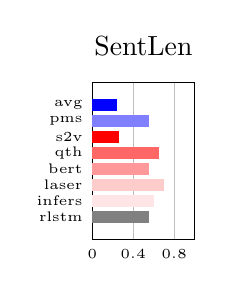
\begin{tikzpicture}

  	\begin{axis}[
		title=SentLen,
 	   	xbar stacked,
		bar width=4pt,
		enlarge y limits=0.2,
    		symbolic y coords={rlstm,infers,laser,bert,qth,s2v,pms,avg},
		xmin=0,xmax=1,
  		xmajorgrids,
		tickwidth=0pt,
		xtick distance=0.40,
  		ytick=data,
		scale only axis=true,
  		width=1.3cm,height=2cm,
		tick label style={font=\tiny}
  	]

		% avg
  		\addplot[blue,fill] coordinates
  			{(0.240,avg) (0.00,pms) (0.00,s2v) (0.00,qth) (0.00,bert) (0.00,laser) (0.00,infers) (0.00,rlstm)};
		% pms
		\addplot[blue!50,fill] coordinates
			{(0.00,avg) (0.553,pms) (0.00,s2v) (0.00,qth) (0.00,bert) (0.00,laser) (0.00,infers) (0.00,rlstm)};

		% s2v
		\addplot[red,fill] coordinates 
			{(0.00,avg) (0.00,pms) (0.254,s2v) (0.00,qth) (0.00,bert) (0.00,laser) (0.00,infers) (0.00,rlstm)};
		% qth
		\addplot[red!60,fill] coordinates
			{(0.00,avg) (0.00,pms) (0.00,s2v) (0.649,qth) (0.00,bert) (0.00,laser) (0.00,infers) (0.00,rlstm)};
		% bert
		\addplot[red!40,fill] coordinates
			{(0.00,avg) (0.00,pms) (0.00,s2v) (0.00,qth) (0.551,bert) (0.00,laser) (0.00,infers) (0.00,rlstm)};
		% laser
		\addplot[red!20,fill] coordinates
			{(0.00,avg) (0.00,pms) (0.00,s2v) (0.00,qth) (0.00,bert) (0.697,laser) (0.00,infers) (0.00,rlstm)};
		% infersent
		\addplot[red!10,fill] coordinates
			{(0.00,avg) (0.00,pms) (0.00,s2v) (0.00,qth) (0.00,bert) (0.00,laser) (0.600,infers) (0.00,rlstm)};

		% rand lstm
		\addplot[gray,fill] coordinates 
			{(0.00,avg) (0.00,pms) (0.00,s2v) (0.00,qth) (0.00,bert) (0.00,laser) (0.00,infers) (0.549,rlstm)};

  	\end{axis}

\end{tikzpicture}
\end{minipage}
\hfill
\begin{minipage}{0.09\textwidth}
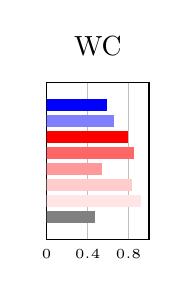
\begin{tikzpicture}

  	\begin{axis}[
		title=WC,
   	 	xbar stacked,
		bar width=4pt,
		enlarge y limits=0.2,
	    	symbolic y coords={rlstm,infers,laser,bert,qth,s2v,pms,avg},
		xmin=0,xmax=1,
  		xmajorgrids,
		tickwidth=0pt,
		xtick distance=0.40,
  		ytick=data,
		yticklabels={,,},
		scale only axis=true,
  		width=1.3cm,height=2cm,
		tick label style={font=\tiny}
  	]

		% avg
  		\addplot[blue,fill] coordinates
  			{(0.581,avg) (0.00,pms) (0.00,s2v) (0.00,qth) (0.00,bert) (0.00,laser) (0.00,infers) (0.00,rlstm)};
		% pms
		\addplot[blue!50,fill] coordinates
			{(0.00,avg) (0.657,pms) (0.00,s2v) (0.00,qth) (0.00,bert) (0.00,laser) (0.00,infers) (0.00,rlstm)};

		% s2v
		\addplot[red,fill] coordinates 
			{(0.00,avg) (0.00,pms) (0.786,s2v) (0.00,qth) (0.00,bert) (0.00,laser) (0.00,infers) (0.00,rlstm)};
		% qth
		\addplot[red!60,fill] coordinates
			{(0.00,avg) (0.00,pms) (0.00,s2v) (0.848,qth) (0.00,bert) (0.00,laser) (0.00,infers) (0.00,rlstm)};
		% bert
		\addplot[red!40,fill] coordinates
			{(0.00,avg) (0.00,pms) (0.00,s2v) (0.00,qth) (0.531,bert) (0.00,laser) (0.00,infers) (0.00,rlstm)};
		% laser
		\addplot[red!20,fill] coordinates
			{(0.00,avg) (0.00,pms) (0.00,s2v) (0.00,qth) (0.00,bert) (0.832,laser) (0.00,infers) (0.00,rlstm)};
		% infersent
		\addplot[red!10,fill] coordinates
			{(0.00,avg) (0.00,pms) (0.00,s2v) (0.00,qth) (0.00,bert) (0.00,laser) (0.919,infers) (0.00,rlstm)};

		% rand lstm
		\addplot[gray,fill] coordinates 
			{(0.00,avg) (0.00,pms) (0.00,s2v) (0.00,qth) (0.00,bert) (0.00,laser) (0.00,infers) (0.462,rlstm)};

  	\end{axis}

\end{tikzpicture}
\end{minipage}
\hfill
\begin{minipage}{0.09\textwidth}
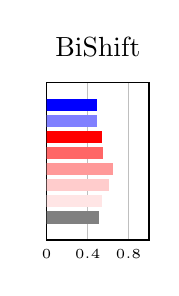
\begin{tikzpicture}

  	\begin{axis}[
		title=BiShift,
 	   	xbar stacked,
		bar width=4pt,
		enlarge y limits=0.2,
    		symbolic y coords={rlstm,infers,laser,bert,qth,s2v,pms,avg},
		xmin=0,xmax=1,
  		xmajorgrids,
		tickwidth=0pt,
		xtick distance=0.40,
  		ytick=data,
		yticklabels={,,},
		scale only axis=true,
  		width=1.3cm,height=2cm,
		tick label style={font=\tiny}
  	]

		% avg
  		\addplot[blue,fill] coordinates
  			{(0.485,avg) (0.00,pms) (0.00,s2v) (0.00,qth) (0.00,bert) (0.00,laser) (0.00,infers) (0.00,rlstm)};
		% pms
		\addplot[blue!50,fill] coordinates
			{(0.00,avg) (0.491,pms) (0.00,s2v) (0.00,qth) (0.00,bert) (0.00,laser) (0.00,infers) (0.00,rlstm)};

		% s2v
		\addplot[red,fill] coordinates 
			{(0.00,avg) (0.00,pms) (0.534,s2v) (0.00,qth) (0.00,bert) (0.00,laser) (0.00,infers) (0.00,rlstm)};
		% qth
		\addplot[red!60,fill] coordinates
			{(0.00,avg) (0.00,pms) (0.00,s2v) (0.544,qth) (0.00,bert) (0.00,laser) (0.00,infers) (0.00,rlstm)};
		% bert
		\addplot[red!40,fill] coordinates
			{(0.00,avg) (0.00,pms) (0.00,s2v) (0.00,qth) (0.641,bert) (0.00,laser) (0.00,infers) (0.00,rlstm)};
		% laser
		\addplot[red!20,fill] coordinates
			{(0.00,avg) (0.00,pms) (0.00,s2v) (0.00,qth) (0.00,bert) (0.600,laser) (0.00,infers) (0.00,rlstm)};
		% infersent
		\addplot[red!10,fill] coordinates
			{(0.00,avg) (0.00,pms) (0.00,s2v) (0.00,qth) (0.00,bert) (0.00,laser) (0.536,infers) (0.00,rlstm)};

		% rand lstm
		\addplot[gray,fill] coordinates 
			{(0.00,avg) (0.00,pms) (0.00,s2v) (0.00,qth) (0.00,bert) (0.00,laser) (0.00,infers) (0.510,rlstm)};

  	\end{axis}

\end{tikzpicture}
\end{minipage}
\hfill
\begin{minipage}{0.09\textwidth}
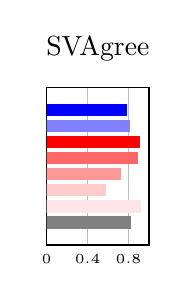
\begin{tikzpicture}

  	\begin{axis}[
		title=SVAgree,
 	   	xbar stacked,
		bar width=4pt,
		enlarge y limits=0.2,
    		symbolic y coords={rlstm,infers,laser,bert,qth,s2v,pms,avg},
		xmin=0,xmax=1,
  		xmajorgrids,
		tickwidth=0pt,
		xtick distance=0.40,
  		ytick=data,
		yticklabels={,,},
		scale only axis=true,
  		width=1.3cm,height=2cm,
		tick label style={font=\tiny}
  	]

		% avg
  		\addplot[blue,fill] coordinates
  			{(0.775,avg) (0.00,pms) (0.00,s2v) (0.00,qth) (0.00,bert) (0.00,laser) (0.00,infers) (0.00,rlstm)};
		% pms
		\addplot[blue!50,fill] coordinates
			{(0.00,avg) (0.804,pms) (0.00,s2v) (0.00,qth) (0.00,bert) (0.00,laser) (0.00,infers) (0.00,rlstm)};

		% s2v
		\addplot[red,fill] coordinates 
			{(0.00,avg) (0.00,pms) (0.910,s2v) (0.00,qth) (0.00,bert) (0.00,laser) (0.00,infers) (0.00,rlstm)};
		% qth
		\addplot[red!60,fill] coordinates
			{(0.00,avg) (0.00,pms) (0.00,s2v) (0.887,qth) (0.00,bert) (0.00,laser) (0.00,infers) (0.00,rlstm)};
		% bert
		\addplot[red!40,fill] coordinates
			{(0.00,avg) (0.00,pms) (0.00,s2v) (0.00,qth) (0.718,bert) (0.00,laser) (0.00,infers) (0.00,rlstm)};
		% laser
		\addplot[red!20,fill] coordinates
			{(0.00,avg) (0.00,pms) (0.00,s2v) (0.00,qth) (0.00,bert) (0.572,laser) (0.00,infers) (0.00,rlstm)};
		% infersent
		\addplot[red!10,fill] coordinates
			{(0.00,avg) (0.00,pms) (0.00,s2v) (0.00,qth) (0.00,bert) (0.00,laser) (0.912,infers) (0.00,rlstm)};

		% rand lstm
		\addplot[gray,fill] coordinates 
			{(0.00,avg) (0.00,pms) (0.00,s2v) (0.00,qth) (0.00,bert) (0.00,laser) (0.00,infers) (0.819,rlstm)};

  	\end{axis}

\end{tikzpicture}
\end{minipage}
\hfill
\begin{minipage}{0.09\textwidth}
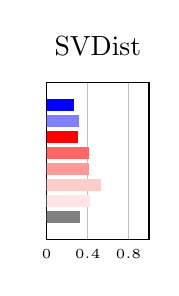
\begin{tikzpicture}

  	\begin{axis}[
		title=SVDist,
  	  	xbar stacked,
		bar width=4pt,
		enlarge y limits=0.2,
    		symbolic y coords={rlstm,infers,laser,bert,qth,s2v,pms,avg},
		xmin=0,xmax=1,
  		xmajorgrids,
		tickwidth=0pt,
		xtick distance=0.40,
  		ytick=data,
		yticklabels={,,},
		scale only axis=true,
  		width=1.3cm,height=2cm,
		tick label style={font=\tiny}
  	]

		% avg
  		\addplot[blue,fill] coordinates
  			{(0.265,avg) (0.00,pms) (0.00,s2v) (0.00,qth) (0.00,bert) (0.00,laser) (0.00,infers) (0.00,rlstm)};
		% pms
		\addplot[blue!50,fill] coordinates
			{(0.00,avg) (0.309,pms) (0.00,s2v) (0.00,qth) (0.00,bert) (0.00,laser) (0.00,infers) (0.00,rlstm)};

		% s2v
		\addplot[red,fill] coordinates 
			{(0.00,avg) (0.00,pms) (0.301,s2v) (0.00,qth) (0.00,bert) (0.00,laser) (0.00,infers) (0.00,rlstm)};
		% qth
		\addplot[red!60,fill] coordinates
			{(0.00,avg) (0.00,pms) (0.00,s2v) (0.410,qth) (0.00,bert) (0.00,laser) (0.00,infers) (0.00,rlstm)};
		% bert
		\addplot[red!40,fill] coordinates
			{(0.00,avg) (0.00,pms) (0.00,s2v) (0.00,qth) (0.406,bert) (0.00,laser) (0.00,infers) (0.00,rlstm)};
		% laser
		\addplot[red!20,fill] coordinates
			{(0.00,avg) (0.00,pms) (0.00,s2v) (0.00,qth) (0.00,bert) (0.521,laser) (0.00,infers) (0.00,rlstm)};
		% infersent
		\addplot[red!10,fill] coordinates
			{(0.00,avg) (0.00,pms) (0.00,s2v) (0.00,qth) (0.00,bert) (0.00,laser) (0.414,infers) (0.00,rlstm)};

		% rand lstm
		\addplot[gray,fill] coordinates 
			{(0.00,avg) (0.00,pms) (0.00,s2v) (0.00,qth) (0.00,bert) (0.00,laser) (0.00,infers) (0.323,rlstm)};

  	\end{axis}

\end{tikzpicture}
\end{minipage}
%\hfill
%\begin{minipage}{0.09\textwidth}
%\begin{tikzpicture}
%
%  	\begin{axis}[
%		title=TC,
% 	   	xbar stacked,
%		bar width=5pt,
%		enlarge y limits=0.2,
%    		symbolic y coords={rlstm,laser,bert,qth,s2v,pms,avg},
%		xmin=0,xmax=1,
%  		xmajorgrids,
%		tickwidth=0pt,
%		xtick distance=0.40,
%  		ytick=data,
%		yticklabels={,,},
%		scale only axis=true,
%  		width=1.3cm,height=2cm,
%		tick label style={font=\tiny}
%  	]
%
%		% avg
%  		\addplot[blue,fill] coordinates
%  			{(0.19,avg) (0.00,pms) (0.00,s2v) (0.00,qth) (0.00,bert) (0.00,laser) (0.00,rlstm)};
%		% pms
%		\addplot[blue!50,fill] coordinates
%			{(0.00,avg) (0.15,pms) (0.00,s2v) (0.00,qth) (0.00,bert) (0.00,laser) (0.00,rlstm)};
%
%		% s2v
%		\addplot[red,fill] coordinates 
%			{(0.00,avg) (0.00,pms) (0.22,s2v) (0.00,qth) (0.00,bert) (0.00,laser) (0.00,rlstm)};
%		% qth
%		\addplot[red!60,fill] coordinates
%			{(0.00,avg) (0.00,pms) (0.00,s2v) (0.30,qth) (0.00,bert) (0.00,laser) (0.00,rlstm)};
%		% bert
%		\addplot[red!40,fill] coordinates
%			{(0.00,avg) (0.00,pms) (0.00,s2v) (0.00,qth) (0.36,bert) (0.00,laser) (0.00,rlstm)};
%		% laser
%		\addplot[red!20,fill] coordinates
%			{(0.00,avg) (0.00,pms) (0.00,s2v) (0.00,qth) (0.00,bert) (0.40,laser) (0.00,rlstm)};
%
%		% rand lstm
%		\addplot[gray,fill] coordinates 
%			{(0.00,avg) (0.00,pms) (0.00,s2v) (0.00,qth) (0.00,bert) (0.00,laser) (0.16,rlstm)};
%
%  	\end{axis}
%
%\end{tikzpicture}
%\end{minipage}
\hfill
\begin{minipage}{0.09\textwidth}
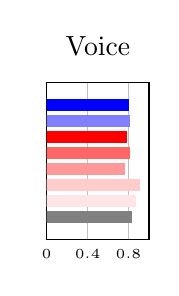
\begin{tikzpicture}

  	\begin{axis}[
		title=Voice,
    		xbar stacked,
		bar width=4pt,
		enlarge y limits=0.2,
    		symbolic y coords={rlstm,infers,laser,bert,qth,s2v,pms,avg},
		xmin=0,xmax=1,
  		xmajorgrids,
		tickwidth=0pt,
		xtick distance=0.40,
  		ytick=data,
		yticklabels={,,},
		scale only axis=true,
  		width=1.3cm,height=2cm,
		tick label style={font=\tiny}
  	]

		% avg
  		\addplot[blue,fill] coordinates
  			{(0.798,avg) (0.00,pms) (0.00,s2v) (0.00,qth) (0.00,bert) (0.00,laser) (0.00,infers) (0.00,rlstm)};
		% pms
		\addplot[blue!50,fill] coordinates
			{(0.00,avg) (0.807,pms) (0.00,s2v) (0.00,qth) (0.00,bert) (0.00,laser) (0.00,infers) (0.00,rlstm)};

		% s2v
		\addplot[red,fill] coordinates 
			{(0.00,avg) (0.00,pms) (0.779,s2v) (0.00,qth) (0.00,bert) (0.00,laser) (0.00,infers) (0.00,rlstm)};
		% qth
		\addplot[red!60,fill] coordinates
			{(0.00,avg) (0.00,pms) (0.00,s2v) (0.811,qth) (0.00,bert) (0.00,laser) (0.00,infers) (0.00,rlstm)};
		% bert
		\addplot[red!40,fill] coordinates
			{(0.00,avg) (0.00,pms) (0.00,s2v) (0.00,qth) (0.760,bert) (0.00,laser) (0.00,infers) (0.00,rlstm)};
		% laser
		\addplot[red!20,fill] coordinates
			{(0.00,avg) (0.00,pms) (0.00,s2v) (0.00,qth) (0.00,bert) (0.904,laser) (0.00,infers) (0.00,rlstm)};
		% infersent
		\addplot[red!10,fill] coordinates
			{(0.00,avg) (0.00,pms) (0.00,s2v) (0.00,qth) (0.00,bert) (0.00,laser) (0.868,infers) (0.00,rlstm)};

		% rand lstm
		\addplot[gray,fill] coordinates 
			{(0.00,avg) (0.00,pms) (0.00,s2v) (0.00,qth) (0.00,bert) (0.00,laser) (0.00,infers) (0.833,rlstm)};

  	\end{axis}

\end{tikzpicture}
\end{minipage}
\hfill
\begin{minipage}{0.09\textwidth}
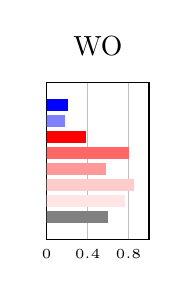
\begin{tikzpicture}

  	\begin{axis}[
		title=WO,
   	 	xbar stacked,
		bar width=4pt,
		enlarge y limits=0.2,
    		symbolic y coords={rlstm,infers,laser,bert,qth,s2v,pms,avg},
		xmin=0,xmax=1,
  		xmajorgrids,
		tickwidth=0pt,
		xtick distance=0.40,
  		ytick=data,
		yticklabels={,,},
		scale only axis=true,
  		width=1.3cm,height=2cm,
		tick label style={font=\tiny}
  	]

		% avg
  		\addplot[blue,fill] coordinates
  			{(0.201,avg) (0.00,pms) (0.00,s2v) (0.00,qth) (0.00,bert) (0.00,laser) (0.00,infers) (0.00,rlstm)};
		% pms
		\addplot[blue!50,fill] coordinates
			{(0.00,avg) (0.173,pms) (0.00,s2v) (0.00,qth) (0.00,bert) (0.00,laser) (0.00,infers) (0.00,rlstm)};

		% s2v
		\addplot[red,fill] coordinates 
			{(0.00,avg) (0.00,pms) (0.381,s2v) (0.00,qth) (0.00,bert) (0.00,laser) (0.00,infers) (0.00,rlstm)};
		% qth
		\addplot[red!60,fill] coordinates
			{(0.00,avg) (0.00,pms) (0.00,s2v) (0.802,qth) (0.00,bert) (0.00,laser) (0.00,infers) (0.00,rlstm)};
		% bert
		\addplot[red!40,fill] coordinates
			{(0.00,avg) (0.00,pms) (0.00,s2v) (0.00,qth) (0.573,bert) (0.00,laser) (0.00,infers) (0.00,rlstm)};
		% laser
		\addplot[red!20,fill] coordinates
			{(0.00,avg) (0.00,pms) (0.00,s2v) (0.00,qth) (0.00,bert) (0.846,laser) (0.00,infers) (0.00,rlstm)};
		% infersent
		\addplot[red!10,fill] coordinates
			{(0.00,avg) (0.00,pms) (0.00,s2v) (0.00,qth) (0.00,bert) (0.00,laser) (0.760,infers) (0.00,rlstm)};

		% rand lstm
		\addplot[gray,fill] coordinates 
			{(0.00,avg) (0.00,pms) (0.00,s2v) (0.00,qth) (0.00,bert) (0.00,laser) (0.00,infers) (0.598,rlstm)};

  	\end{axis}

\end{tikzpicture}
\end{minipage}
\hfill
\begin{minipage}{0.09\textwidth}
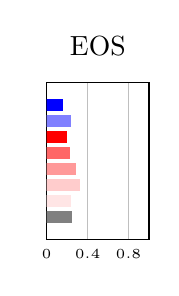
\begin{tikzpicture}

  	\begin{axis}[
		title=EOS,
  	  	xbar stacked,
		bar width=4pt,
		enlarge y limits=0.2,
    		symbolic y coords={rlstm,infers,laser,bert,qth,s2v,pms,avg},
		xmin=0,xmax=1,
  		xmajorgrids,
		tickwidth=0pt,
		xtick distance=0.40,
  		ytick=data,
		yticklabels={,,},
		scale only axis=true,
  		width=1.3cm,height=2cm,
		tick label style={font=\tiny}
  	]

		% avg
  		\addplot[blue,fill] coordinates
  			{(0.150,avg) (0.00,pms) (0.00,s2v) (0.00,qth) (0.00,bert) (0.00,laser) (0.00,infers) (0.00,rlstm)};
		% pms
		\addplot[blue!50,fill] coordinates
			{(0.00,avg) (0.231,pms) (0.00,s2v) (0.00,qth) (0.00,bert) (0.00,laser) (0.00,infers) (0.00,rlstm)};

		% s2v
		\addplot[red,fill] coordinates 
			{(0.00,avg) (0.00,pms) (0.191,s2v) (0.00,qth) (0.00,bert) (0.00,laser) (0.00,infers) (0.00,rlstm)};
		% qth
		\addplot[red!60,fill] coordinates
			{(0.00,avg) (0.00,pms) (0.00,s2v) (0.221,qth) (0.00,bert) (0.00,laser) (0.00,infers) (0.00,rlstm)};
		% bert
		\addplot[red!40,fill] coordinates
			{(0.00,avg) (0.00,pms) (0.00,s2v) (0.00,qth) (0.282,bert) (0.00,laser) (0.00,infers) (0.00,rlstm)};
		% laser
		\addplot[red!20,fill] coordinates
			{(0.00,avg) (0.00,pms) (0.00,s2v) (0.00,qth) (0.00,bert) (0.319,laser) (0.00,infers) (0.00,rlstm)};
		% infersent
		\addplot[red!10,fill] coordinates
			{(0.00,avg) (0.00,pms) (0.00,s2v) (0.00,qth) (0.00,bert) (0.00,laser) (0.230,infers) (0.00,rlstm)};

		% rand lstm
		\addplot[gray,fill] coordinates 
			{(0.00,avg) (0.00,pms) (0.00,s2v) (0.00,qth) (0.00,bert) (0.00,laser) (0.00,infers) (0.246,rlstm)};

  	\end{axis}

\end{tikzpicture}
\end{minipage}
\hfill
\begin{minipage}{0.09\textwidth}
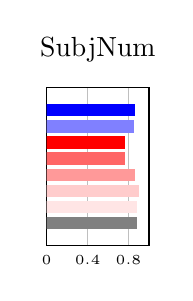
\begin{tikzpicture}

  	\begin{axis}[
		title=SubjNum,
    		xbar stacked,
		bar width=4pt,
		enlarge y limits=0.2,
    		symbolic y coords={rlstm,infers,laser,bert,qth,s2v,pms,avg},
		xmin=0,xmax=1,
  		xmajorgrids,
		tickwidth=0pt,
		xtick distance=0.40,
  		ytick=data,
		yticklabels={,,},
		scale only axis=true,
  		width=1.3cm,height=2cm,
		tick label style={font=\tiny}
  	]

		% avg
  		\addplot[blue,fill] coordinates
  			{(0.855,avg) (0.00,pms) (0.00,s2v) (0.00,qth) (0.00,bert) (0.00,laser) (0.00,infers) (0.00,rlstm)};
		% pms
		\addplot[blue!50,fill] coordinates
			{(0.00,avg) (0.850,pms) (0.00,s2v) (0.00,qth) (0.00,bert) (0.00,laser) (0.00,infers) (0.00,rlstm)};

		% s2v
		\addplot[red,fill] coordinates 
			{(0.00,avg) (0.00,pms) (0.759,s2v) (0.00,qth) (0.00,bert) (0.00,laser) (0.00,infers) (0.00,rlstm)};
		% qth
		\addplot[red!60,fill] coordinates
			{(0.00,avg) (0.00,pms) (0.00,s2v) (0.758,qth) (0.00,bert) (0.00,laser) (0.00,infers) (0.00,rlstm)};
		% bert
		\addplot[red!40,fill] coordinates
			{(0.00,avg) (0.00,pms) (0.00,s2v) (0.00,qth) (0.858,bert) (0.00,laser) (0.00,infers) (0.00,rlstm)};
		% laser
		\addplot[red!20,fill] coordinates
			{(0.00,avg) (0.00,pms) (0.00,s2v) (0.00,qth) (0.00,bert) (0.899,laser) (0.00,infers) (0.00,rlstm)};
		% infersent
		\addplot[red!10,fill] coordinates
			{(0.00,avg) (0.00,pms) (0.00,s2v) (0.00,qth) (0.00,bert) (0.00,laser) (0.879,infers) (0.00,rlstm)};

		% rand lstm
		\addplot[gray,fill] coordinates 
			{(0.00,avg) (0.00,pms) (0.00,s2v) (0.00,qth) (0.00,bert) (0.00,laser) (0.00,infers) (0.879,rlstm)};

  	\end{axis}

\end{tikzpicture}
\end{minipage}
\begin{center}
$\uparrow$ English
\end{center}
\begin{minipage}{0.115\textwidth}
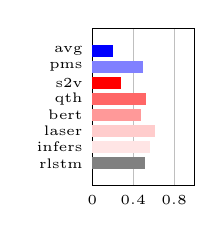
\begin{tikzpicture}

  	\begin{axis}[
    	xbar stacked,
		bar width=4pt,
		enlarge y limits=0.2,
    		symbolic y coords={rlstm,infers,laser,bert,qth,s2v,pms,avg},
		xmin=0,xmax=1,
  		xmajorgrids,
		tickwidth=0pt,
		xtick distance=0.40,
  		ytick=data,
		scale only axis=true,
  		width=1.3cm,height=2cm,
		tick label style={font=\tiny}
  	]

		% avg
  		\addplot[blue,fill] coordinates
  			{(0.195,avg) (0.00,pms) (0.00,s2v) (0.00,qth) (0.00,bert) (0.00,laser) (0.00,infers) (0.00,rlstm)};
		% pms
		\addplot[blue!50,fill] coordinates
			{(0.00,avg) (0.492,pms) (0.00,s2v) (0.00,qth) (0.00,bert) (0.00,laser) (0.00,infers) (0.00,rlstm)};

		% s2v
		\addplot[red,fill] coordinates 
			{(0.00,avg) (0.00,pms) (0.271,s2v) (0.00,qth) (0.00,bert) (0.00,laser) (0.00,infers) (0.00,rlstm)};
		% qth
		\addplot[red!60,fill] coordinates
			{(0.00,avg) (0.00,pms) (0.00,s2v) (0.520,qth) (0.00,bert) (0.00,laser) (0.00,infers) (0.00,rlstm)};
		% bert
		\addplot[red!40,fill] coordinates
			{(0.00,avg) (0.00,pms) (0.00,s2v) (0.00,qth) (0.467,bert) (0.00,laser) (0.00,infers) (0.00,rlstm)};
		% laser
		\addplot[red!20,fill] coordinates
			{(0.00,avg) (0.00,pms) (0.00,s2v) (0.00,qth) (0.00,bert) (0.608,laser) (0.00,infers) (0.00,rlstm)};
		% infersent
		\addplot[red!10,fill] coordinates
			{(0.00,avg) (0.00,pms) (0.00,s2v) (0.00,qth) (0.00,bert) (0.00,laser) (0.557,infers) (0.00,rlstm)};

		% rand lstm
		\addplot[gray,fill] coordinates 
			{(0.00,avg) (0.00,pms) (0.00,s2v) (0.00,qth) (0.00,bert) (0.00,laser) (0.00,infers) (0.508,rlstm)};

  	\end{axis}

\end{tikzpicture}
\end{minipage}
\hfill
\begin{minipage}{0.09\textwidth}
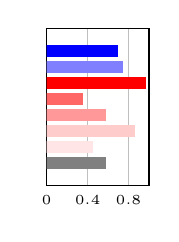
\begin{tikzpicture}

  	\begin{axis}[
    	xbar stacked,
		bar width=4pt,
		enlarge y limits=0.2,
    		symbolic y coords={rlstm,infers,laser,bert,qth,s2v,pms,avg},
		xmin=0,xmax=1,
  		xmajorgrids,
		tickwidth=0pt,
		xtick distance=0.40,
  		ytick=data,
		yticklabels={,,},
		scale only axis=true,
  		width=1.3cm,height=2cm,
		tick label style={font=\tiny}
  	]

		% avg
  		\addplot[blue,fill] coordinates
  			{(0.695,avg) (0.00,pms) (0.00,s2v) (0.00,qth) (0.00,bert) (0.00,laser) (0.00,infers) (0.00,rlstm)};
		% pms
		\addplot[blue!50,fill] coordinates
			{(0.00,avg) (0.745,pms) (0.00,s2v) (0.00,qth) (0.00,bert) (0.00,laser) (0.00,infers) (0.00,rlstm)};

		% s2v
		\addplot[red,fill] coordinates 
			{(0.00,avg) (0.00,pms) (0.968,s2v) (0.00,qth) (0.00,bert) (0.00,laser) (0.00,infers) (0.00,rlstm)};
		% qth
		\addplot[red!60,fill] coordinates
			{(0.00,avg) (0.00,pms) (0.00,s2v) (0.346,qth) (0.00,bert) (0.00,laser) (0.00,infers) (0.00,rlstm)};
		% bert
		\addplot[red!40,fill] coordinates
			{(0.00,avg) (0.00,pms) (0.00,s2v) (0.00,qth) (0.577,bert) (0.00,laser) (0.00,infers) (0.00,rlstm)};
		% laser
		\addplot[red!20,fill] coordinates
			{(0.00,avg) (0.00,pms) (0.00,s2v) (0.00,qth) (0.00,bert) (0.861,laser) (0.00,infers) (0.00,rlstm)};
		% infersent
		\addplot[red!10,fill] coordinates
			{(0.00,avg) (0.00,pms) (0.00,s2v) (0.00,qth) (0.00,bert) (0.00,laser) (0.449,infers) (0.00,rlstm)};

		% rand lstm
		\addplot[gray,fill] coordinates 
			{(0.00,avg) (0.00,pms) (0.00,s2v) (0.00,qth) (0.00,bert) (0.00,laser) (0.00,infers) (0.577,rlstm)};

  	\end{axis}

\end{tikzpicture}
\end{minipage}
\hfill
\begin{minipage}{0.09\textwidth}
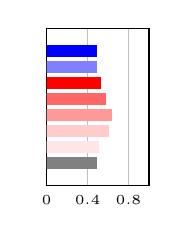
\begin{tikzpicture}

  	\begin{axis}[
    		xbar stacked,
		bar width=4pt,
		enlarge y limits=0.2,
    		symbolic y coords={rlstm,infers,laser,bert,qth,s2v,pms,avg},
		xmin=0,xmax=1,
  		xmajorgrids,
		tickwidth=0pt,
		xtick distance=0.40,
  		ytick=data,
		yticklabels={,,},
		scale only axis=true,
  		width=1.3cm,height=2cm,
		tick label style={font=\tiny}
  	]

		% avg
  		\addplot[blue,fill] coordinates
  			{(0.489,avg) (0.00,pms) (0.00,s2v) (0.00,qth) (0.00,bert) (0.00,laser) (0.00,infers) (0.00,rlstm)};
		% pms
		\addplot[blue!50,fill] coordinates
			{(0.00,avg) (0.489,pms) (0.00,s2v) (0.00,qth) (0.00,bert) (0.00,laser) (0.00,infers) (0.00,rlstm)};

		% s2v
		\addplot[red,fill] coordinates 
			{(0.00,avg) (0.00,pms) (0.521,s2v) (0.00,qth) (0.00,bert) (0.00,laser) (0.00,infers) (0.00,rlstm)};
		% qth
		\addplot[red!60,fill] coordinates
			{(0.00,avg) (0.00,pms) (0.00,s2v) (0.575,qth) (0.00,bert) (0.00,laser) (0.00,infers) (0.00,rlstm)};
		% bert
		\addplot[red!40,fill] coordinates
			{(0.00,avg) (0.00,pms) (0.00,s2v) (0.00,qth) (0.636,bert) (0.00,laser) (0.00,infers) (0.00,rlstm)};
		% laser
		\addplot[red!20,fill] coordinates
			{(0.00,avg) (0.00,pms) (0.00,s2v) (0.00,qth) (0.00,bert) (0.606,laser) (0.00,infers) (0.00,rlstm)};
		% infersent
		\addplot[red!10,fill] coordinates
			{(0.00,avg) (0.00,pms) (0.00,s2v) (0.00,qth) (0.00,bert) (0.00,laser) (0.505,infers) (0.00,rlstm)};

		% rand lstm
		\addplot[gray,fill] coordinates 
			{(0.00,avg) (0.00,pms) (0.00,s2v) (0.00,qth) (0.00,bert) (0.00,laser) (0.00,infers) (0.490,rlstm)};

  	\end{axis}

\end{tikzpicture}
\end{minipage}
\hfill
\begin{minipage}{0.09\textwidth}
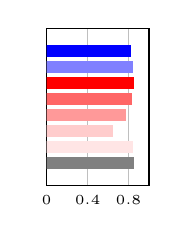
\begin{tikzpicture}

  	\begin{axis}[
   	 	xbar stacked,
		bar width=4pt,
		enlarge y limits=0.2,
    		symbolic y coords={rlstm,infers,laser,bert,qth,s2v,pms,avg},
		xmin=0,xmax=1,
  		xmajorgrids,
		tickwidth=0pt,
		xtick distance=0.40,
  		ytick=data,
		yticklabels={,,},
		scale only axis=true,
  		width=1.3cm,height=2cm,
		tick label style={font=\tiny}
  	]

		% avg
  		\addplot[blue,fill] coordinates
  			{(0.822,avg) (0.00,pms) (0.00,s2v) (0.00,qth) (0.00,bert) (0.00,laser) (0.00,infers) (0.00,rlstm)};
		% pms
		\addplot[blue!50,fill] coordinates
			{(0.00,avg) (0.837,pms) (0.00,s2v) (0.00,qth) (0.00,bert) (0.00,laser) (0.00,infers) (0.00,rlstm)};

		% s2v
		\addplot[red,fill] coordinates 
			{(0.00,avg) (0.00,pms) (0.845,s2v) (0.00,qth) (0.00,bert) (0.00,laser) (0.00,infers) (0.00,rlstm)};
		% qth
		\addplot[red!60,fill] coordinates
			{(0.00,avg) (0.00,pms) (0.00,s2v) (0.825,qth) (0.00,bert) (0.00,laser) (0.00,infers) (0.00,rlstm)};
		% bert
		\addplot[red!40,fill] coordinates
			{(0.00,avg) (0.00,pms) (0.00,s2v) (0.00,qth) (0.771,bert) (0.00,laser) (0.00,infers) (0.00,rlstm)};
		% laser
		\addplot[red!20,fill] coordinates
			{(0.00,avg) (0.00,pms) (0.00,s2v) (0.00,qth) (0.00,bert) (0.639,laser) (0.00,infers) (0.00,rlstm)};
		% infersent
		\addplot[red!10,fill] coordinates
			{(0.00,avg) (0.00,pms) (0.00,s2v) (0.00,qth) (0.00,bert) (0.00,laser) (0.834,infers) (0.00,rlstm)};

		% rand lstm
		\addplot[gray,fill] coordinates 
			{(0.00,avg) (0.00,pms) (0.00,s2v) (0.00,qth) (0.00,bert) (0.00,laser) (0.00,infers) (0.847,rlstm)};

  	\end{axis}

\end{tikzpicture}
\end{minipage}
\hfill
\begin{minipage}{0.09\textwidth}
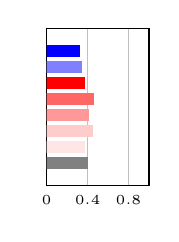
\begin{tikzpicture}

  	\begin{axis}[
    		xbar stacked,
		bar width=4pt,
		enlarge y limits=0.2,
    		symbolic y coords={rlstm,infers,laser,bert,qth,s2v,pms,avg},
		xmin=0,xmax=1,
  		xmajorgrids,
		tickwidth=0pt,
		xtick distance=0.40,
  		ytick=data,
		yticklabels={,,},
		scale only axis=true,
  		width=1.3cm,height=2cm,
		tick label style={font=\tiny}
  	]

		% avg
  		\addplot[blue,fill] coordinates
  			{(0.318,avg) (0.00,pms) (0.00,s2v) (0.00,qth) (0.00,bert) (0.00,laser) (0.00,infers) (0.00,rlstm)};
		% pms
		\addplot[blue!50,fill] coordinates
			{(0.00,avg) (0.336,pms) (0.00,s2v) (0.00,qth) (0.00,bert) (0.00,laser) (0.00,infers) (0.00,rlstm)};

		% s2v
		\addplot[red,fill] coordinates 
			{(0.00,avg) (0.00,pms) (0.370,s2v) (0.00,qth) (0.00,bert) (0.00,laser) (0.00,infers) (0.00,rlstm)};
		% qth
		\addplot[red!60,fill] coordinates
			{(0.00,avg) (0.00,pms) (0.00,s2v) (0.456,qth) (0.00,bert) (0.00,laser) (0.00,infers) (0.00,rlstm)};
		% bert
		\addplot[red!40,fill] coordinates
			{(0.00,avg) (0.00,pms) (0.00,s2v) (0.00,qth) (0.404,bert) (0.00,laser) (0.00,infers) (0.00,rlstm)};
		% laser
		\addplot[red!20,fill] coordinates
			{(0.00,avg) (0.00,pms) (0.00,s2v) (0.00,qth) (0.00,bert) (0.448,laser) (0.00,infers) (0.00,rlstm)};
		% infersent
		\addplot[red!10,fill] coordinates
			{(0.00,avg) (0.00,pms) (0.00,s2v) (0.00,qth) (0.00,bert) (0.00,laser) (0.367,infers) (0.00,rlstm)};

		% rand lstm
		\addplot[gray,fill] coordinates 
			{(0.00,avg) (0.00,pms) (0.00,s2v) (0.00,qth) (0.00,bert) (0.00,laser) (0.00,infers) (0.399,rlstm)};

  	\end{axis}

\end{tikzpicture}
\end{minipage}
%\hfill
%\begin{minipage}{0.09\textwidth}
%\begin{tikzpicture}
%
%  	\begin{axis}[
%   	 	xbar stacked,
%		bar width=5pt,
%		enlarge y limits=0.2,
%    		symbolic y coords={rlstm,laser,bert,qth,s2v,pms,avg},
%		xmin=0,xmax=1,
%  		xmajorgrids,
%		tickwidth=0pt,
%		xtick distance=0.40,
%  		ytick=data,
%		yticklabels={,,},
%		scale only axis=true,
%  		width=1.3cm,height=2cm,
%		tick label style={font=\tiny}
%  	]
%
%		% avg
%  		\addplot[blue,fill] coordinates
%  			{(0.42,avg) (0.00,pms) (0.00,s2v) (0.00,qth) (0.00,bert) (0.00,laser) (0.00,rlstm)};
%		% pms
%		\addplot[blue!50,fill] coordinates
%			{(0.00,avg) (0.40,pms) (0.00,s2v) (0.00,qth) (0.00,bert) (0.00,laser) (0.00,rlstm)};
%
%		% s2v
%		\addplot[red,fill] coordinates 
%			{(0.00,avg) (0.00,pms) (0.54,s2v) (0.00,qth) (0.00,bert) (0.00,laser) (0.00,rlstm)};
%		% qth
%		\addplot[red!60,fill] coordinates
%			{(0.00,avg) (0.00,pms) (0.00,s2v) (0.56,qth) (0.00,bert) (0.00,laser) (0.00,rlstm)};
%		% bert
%		\addplot[red!40,fill] coordinates
%			{(0.00,avg) (0.00,pms) (0.00,s2v) (0.00,qth) (0.52,bert) (0.00,laser) (0.00,rlstm)};
%		% laser
%		\addplot[red!20,fill] coordinates
%			{(0.00,avg) (0.00,pms) (0.00,s2v) (0.00,qth) (0.00,bert) (0.58,laser) (0.00,rlstm)};
%
%		% rand lstm
%		\addplot[gray,fill] coordinates 
%			{(0.00,avg) (0.00,pms) (0.00,s2v) (0.00,qth) (0.00,bert) (0.00,laser) (0.35,rlstm)};
%
%  	\end{axis}
%
%\end{tikzpicture}
%\end{minipage}
\hfill
\begin{minipage}{0.09\textwidth}
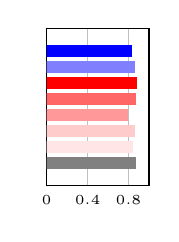
\begin{tikzpicture}

  	\begin{axis}[
    		xbar stacked,
		bar width=4pt,
		enlarge y limits=0.2,
  	  	symbolic y coords={rlstm,infers,laser,bert,qth,s2v,pms,avg},
		xmin=0,xmax=1,
  		xmajorgrids,
		tickwidth=0pt,
		xtick distance=0.40,
  		ytick=data,
		yticklabels={,,},
		scale only axis=true,
  		width=1.3cm,height=2cm,
		tick label style={font=\tiny}
  	]

		% avg
  		\addplot[blue,fill] coordinates
  			{(0.832,avg) (0.00,pms) (0.00,s2v) (0.00,qth) (0.00,bert) (0.00,laser) (0.00,infers) (0.00,rlstm)};
		% pms
		\addplot[blue!50,fill] coordinates
			{(0.00,avg) (0.856,pms) (0.00,s2v) (0.00,qth) (0.00,bert) (0.00,laser) (0.00,infers) (0.00,rlstm)};

		% s2v
		\addplot[red,fill] coordinates 
			{(0.00,avg) (0.00,pms) (0.874,s2v) (0.00,qth) (0.00,bert) (0.00,laser) (0.00,infers) (0.00,rlstm)};
		% qth
		\addplot[red!60,fill] coordinates
			{(0.00,avg) (0.00,pms) (0.00,s2v) (0.868,qth) (0.00,bert) (0.00,laser) (0.00,infers) (0.00,rlstm)};
		% bert
		\addplot[red!40,fill] coordinates
			{(0.00,avg) (0.00,pms) (0.00,s2v) (0.00,qth) (0.793,bert) (0.00,laser) (0.00,infers) (0.00,rlstm)};
		% laser
		\addplot[red!20,fill] coordinates
			{(0.00,avg) (0.00,pms) (0.00,s2v) (0.00,qth) (0.00,bert) (0.854,laser) (0.00,infers) (0.00,rlstm)};
		% infersent
		\addplot[red!10,fill] coordinates
			{(0.00,avg) (0.00,pms) (0.00,s2v) (0.00,qth) (0.00,bert) (0.00,laser) (0.838,infers) (0.00,rlstm)};

		% rand lstm
		\addplot[gray,fill] coordinates 
			{(0.00,avg) (0.00,pms) (0.00,s2v) (0.00,qth) (0.00,bert) (0.00,laser) (0.00,infers) (0.864,rlstm)};

  	\end{axis}

\end{tikzpicture}
\end{minipage}
\hfill
\begin{minipage}{0.09\textwidth}
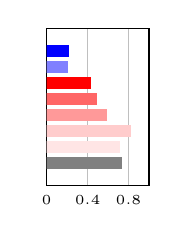
\begin{tikzpicture}

  	\begin{axis}[
   	 	xbar stacked,
		bar width=4pt,
		enlarge y limits=0.2,
   	 	symbolic y coords={rlstm,infers,laser,bert,qth,s2v,pms,avg},
		xmin=0,xmax=1,
  		xmajorgrids,
		tickwidth=0pt,
		xtick distance=0.40,
  		ytick=data,
		yticklabels={,,},
		scale only axis=true,
  		width=1.3cm,height=2cm,
		tick label style={font=\tiny}
  	]

		% avg
  		\addplot[blue,fill] coordinates
  			{(0.215,avg) (0.00,pms) (0.00,s2v) (0.00,qth) (0.00,bert) (0.00,laser) (0.00,infers) (0.00,rlstm)};
		% pms
		\addplot[blue!50,fill] coordinates
			{(0.00,avg) (0.199,pms) (0.00,s2v) (0.00,qth) (0.00,bert) (0.00,laser) (0.00,infers) (0.00,rlstm)};

		% s2v
		\addplot[red,fill] coordinates 
			{(0.00,avg) (0.00,pms) (0.429,s2v) (0.00,qth) (0.00,bert) (0.00,laser) (0.00,infers) (0.00,rlstm)};
		% qth
		\addplot[red!60,fill] coordinates
			{(0.00,avg) (0.00,pms) (0.00,s2v) (0.490,qth) (0.00,bert) (0.00,laser) (0.00,infers) (0.00,rlstm)};
		% bert
		\addplot[red!40,fill] coordinates
			{(0.00,avg) (0.00,pms) (0.00,s2v) (0.00,qth) (0.584,bert) (0.00,laser) (0.00,infers) (0.00,rlstm)};
		% laser
		\addplot[red!20,fill] coordinates
			{(0.00,avg) (0.00,pms) (0.00,s2v) (0.00,qth) (0.00,bert) (0.821,laser) (0.00,infers) (0.00,rlstm)};
		% infersent
		\addplot[red!10,fill] coordinates
			{(0.00,avg) (0.00,pms) (0.00,s2v) (0.00,qth) (0.00,bert) (0.00,laser) (0.713,infers) (0.00,rlstm)};

		% rand lstm
		\addplot[gray,fill] coordinates 
			{(0.00,avg) (0.00,pms) (0.00,s2v) (0.00,qth) (0.00,bert) (0.00,laser) (0.00,infers) (0.735,rlstm)};

  	\end{axis}

\end{tikzpicture}
\end{minipage}
\hfill
\begin{minipage}{0.09\textwidth}
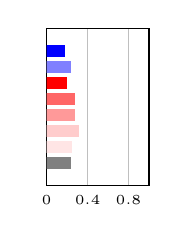
\begin{tikzpicture}

  	\begin{axis}[
   	 	xbar stacked,
		bar width=4pt,
		enlarge y limits=0.2,
    		symbolic y coords={rlstm,infers,laser,bert,qth,s2v,pms,avg},
		xmin=0,xmax=1,
  		xmajorgrids,
		tickwidth=0pt,
		xtick distance=0.40,
  		ytick=data,
		yticklabels={,,},
		scale only axis=true,
  		width=1.3cm,height=2cm,
		tick label style={font=\tiny}
  	]

		% avg
  		\addplot[blue,fill] coordinates
  			{(0.172,avg) (0.00,pms) (0.00,s2v) (0.00,qth) (0.00,bert) (0.00,laser) (0.00,infers) (0.00,rlstm)};
		% pms
		\addplot[blue!50,fill] coordinates
			{(0.00,avg) (0.232,pms) (0.00,s2v) (0.00,qth) (0.00,bert) (0.00,laser) (0.00,infers) (0.00,rlstm)};

		% s2v
		\addplot[red,fill] coordinates 
			{(0.00,avg) (0.00,pms) (0.197,s2v) (0.00,qth) (0.00,bert) (0.00,laser) (0.00,infers) (0.00,rlstm)};
		% qth
		\addplot[red!60,fill] coordinates
			{(0.00,avg) (0.00,pms) (0.00,s2v) (0.269,qth) (0.00,bert) (0.00,laser) (0.00,infers) (0.00,rlstm)};
		% bert
		\addplot[red!40,fill] coordinates
			{(0.00,avg) (0.00,pms) (0.00,s2v) (0.00,qth) (0.269,bert) (0.00,laser) (0.00,infers) (0.00,rlstm)};
		% laser
		\addplot[red!20,fill] coordinates
			{(0.00,avg) (0.00,pms) (0.00,s2v) (0.00,qth) (0.00,bert) (0.307,laser) (0.00,infers) (0.00,rlstm)};
		% infersent
		\addplot[red!10,fill] coordinates
			{(0.00,avg) (0.00,pms) (0.00,s2v) (0.00,qth) (0.00,bert) (0.00,laser) (0.242,infers) (0.00,rlstm)};

		% rand lstm
		\addplot[gray,fill] coordinates 
			{(0.00,avg) (0.00,pms) (0.00,s2v) (0.00,qth) (0.00,bert) (0.00,laser) (0.00,infers) (0.229,rlstm)};

  	\end{axis}

\end{tikzpicture}
\end{minipage}
\hfill
\begin{minipage}{0.09\textwidth}
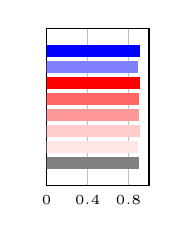
\begin{tikzpicture}

  	\begin{axis}[
 	   	xbar stacked,
		bar width=4pt,
		enlarge y limits=0.2,
   	 	symbolic y coords={rlstm,infers,laser,bert,qth,s2v,pms,avg},
		xmin=0,xmax=1,
  		xmajorgrids,
		tickwidth=0pt,
		xtick distance=0.40,
  		ytick=data,
		yticklabels={,,},
		scale only axis=true,
  		width=1.3cm,height=2cm,
		tick label style={font=\tiny}
  	]

		% avg
  		\addplot[blue,fill] coordinates
  			{(0.903,avg) (0.00,pms) (0.00,s2v) (0.00,qth) (0.00,bert) (0.00,laser) (0.00,infers) (0.00,rlstm)};
		% pms
		\addplot[blue!50,fill] coordinates
			{(0.00,avg) (0.890,pms) (0.00,s2v) (0.00,qth) (0.00,bert) (0.00,laser) (0.00,infers) (0.00,rlstm)};

		% s2v
		\addplot[red,fill] coordinates 
			{(0.00,avg) (0.00,pms) (0.906,s2v) (0.00,qth) (0.00,bert) (0.00,laser) (0.00,infers) (0.00,rlstm)};
		% qth
		\addplot[red!60,fill] coordinates
			{(0.00,avg) (0.00,pms) (0.00,s2v) (0.901,qth) (0.00,bert) (0.00,laser) (0.00,infers) (0.00,rlstm)};
		% bert
		\addplot[red!40,fill] coordinates
			{(0.00,avg) (0.00,pms) (0.00,s2v) (0.00,qth) (0.896,bert) (0.00,laser) (0.00,infers) (0.00,rlstm)};
		% laser
		\addplot[red!20,fill] coordinates
			{(0.00,avg) (0.00,pms) (0.00,s2v) (0.00,qth) (0.00,bert) (0.905,laser) (0.00,infers) (0.00,rlstm)};
		% infersent
		\addplot[red!10,fill] coordinates
			{(0.00,avg) (0.00,pms) (0.00,s2v) (0.00,qth) (0.00,bert) (0.00,laser) (0.882,infers) (0.00,rlstm)};

		% rand lstm
		\addplot[gray,fill] coordinates 
			{(0.00,avg) (0.00,pms) (0.00,s2v) (0.00,qth) (0.00,bert) (0.00,laser) (0.00,infers) (0.895,rlstm)};

  	\end{axis}

\end{tikzpicture}
\end{minipage}
\begin{center}
$\uparrow$ German
\end{center}
\begin{minipage}{0.115\textwidth}
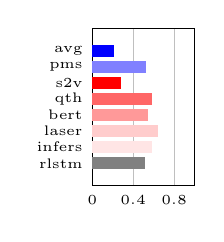
\begin{tikzpicture}

  	\begin{axis}[
    	xbar stacked,
		bar width=4pt,
		enlarge y limits=0.2,
    		symbolic y coords={rlstm,infers,laser,bert,qth,s2v,pms,avg},
		xmin=0,xmax=1,
  		xmajorgrids,
		tickwidth=0pt,
		xtick distance=0.40,
  		ytick=data,
		scale only axis=true,
  		width=1.3cm,height=2cm,
		tick label style={font=\tiny}
  	]

		% avg
  		\addplot[blue,fill] coordinates
  			{(0.208,avg) (0.00,pms) (0.00,s2v) (0.00,qth) (0.00,bert) (0.00,laser) (0.00,infers) (0.00,rlstm)};
		% pms
		\addplot[blue!50,fill] coordinates
			{(0.00,avg) (0.519,pms) (0.00,s2v) (0.00,qth) (0.00,bert) (0.00,laser) (0.00,infers) (0.00,rlstm)};

		% s2v
		\addplot[red,fill] coordinates 
			{(0.00,avg) (0.00,pms) (0.273,s2v) (0.00,qth) (0.00,bert) (0.00,laser) (0.00,infers) (0.00,rlstm)};
		% qth
		\addplot[red!60,fill] coordinates
			{(0.00,avg) (0.00,pms) (0.00,s2v) (0.574,qth) (0.00,bert) (0.00,laser) (0.00,infers) (0.00,rlstm)};
		% bert
		\addplot[red!40,fill] coordinates
			{(0.00,avg) (0.00,pms) (0.00,s2v) (0.00,qth) (0.540,bert) (0.00,laser) (0.00,infers) (0.00,rlstm)};
		% laser
		\addplot[red!20,fill] coordinates
			{(0.00,avg) (0.00,pms) (0.00,s2v) (0.00,qth) (0.00,bert) (0.636,laser) (0.00,infers) (0.00,rlstm)};
		% infersent
		\addplot[red!10,fill] coordinates
			{(0.00,avg) (0.00,pms) (0.00,s2v) (0.00,qth) (0.00,bert) (0.00,laser) (0.576,infers) (0.00,rlstm)};

		% rand lstm
		\addplot[gray,fill] coordinates 
			{(0.00,avg) (0.00,pms) (0.00,s2v) (0.00,qth) (0.00,bert) (0.00,laser) (0.00,infers) (0.515,rlstm)};

  	\end{axis}

\end{tikzpicture}
\end{minipage}
\hfill
\begin{minipage}{0.09\textwidth}
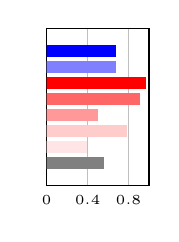
\begin{tikzpicture}

  	\begin{axis}[
    	xbar stacked,
		bar width=4pt,
		enlarge y limits=0.2,
    		symbolic y coords={rlstm,infers,laser,bert,qth,s2v,pms,avg},
		xmin=0,xmax=1,
  		xmajorgrids,
		tickwidth=0pt,
		xtick distance=0.40,
  		ytick=data,
		yticklabels={,,},
		scale only axis=true,
  		width=1.3cm,height=2cm,
		tick label style={font=\tiny}
  	]

		% avg
  		\addplot[blue,fill] coordinates
  			{(0.672,avg) (0.00,pms) (0.00,s2v) (0.00,qth) (0.00,bert) (0.00,laser) (0.00,infers) (0.00,rlstm)};
		% pms
		\addplot[blue!50,fill] coordinates
			{(0.00,avg) (0.673,pms) (0.00,s2v) (0.00,qth) (0.00,bert) (0.00,laser) (0.00,infers) (0.00,rlstm)};

		% s2v
		\addplot[red,fill] coordinates 
			{(0.00,avg) (0.00,pms) (0.968,s2v) (0.00,qth) (0.00,bert) (0.00,laser) (0.00,infers) (0.00,rlstm)};
		% qth
		\addplot[red!60,fill] coordinates
			{(0.00,avg) (0.00,pms) (0.00,s2v) (0.904,qth) (0.00,bert) (0.00,laser) (0.00,infers) (0.00,rlstm)};
		% bert
		\addplot[red!40,fill] coordinates
			{(0.00,avg) (0.00,pms) (0.00,s2v) (0.00,qth) (0.495,bert) (0.00,laser) (0.00,infers) (0.00,rlstm)};
		% laser
		\addplot[red!20,fill] coordinates
			{(0.00,avg) (0.00,pms) (0.00,s2v) (0.00,qth) (0.00,bert) (0.776,laser) (0.00,infers) (0.00,rlstm)};
		% infersent
		\addplot[red!10,fill] coordinates
			{(0.00,avg) (0.00,pms) (0.00,s2v) (0.00,qth) (0.00,bert) (0.00,laser) (0.389,infers) (0.00,rlstm)};

		% rand lstm
		\addplot[gray,fill] coordinates 
			{(0.00,avg) (0.00,pms) (0.00,s2v) (0.00,qth) (0.00,bert) (0.00,laser) (0.00,infers) (0.552,rlstm)};

  	\end{axis}

\end{tikzpicture}
\end{minipage}
\hfill
\begin{minipage}{0.09\textwidth}
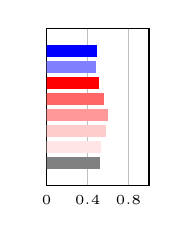
\begin{tikzpicture}

  	\begin{axis}[
    		xbar stacked,
		bar width=4pt,
		enlarge y limits=0.2,
    		symbolic y coords={rlstm,infers,laser,bert,qth,s2v,pms,avg},
		xmin=0,xmax=1,
  		xmajorgrids,
		tickwidth=0pt,
		xtick distance=0.40,
  		ytick=data,
		yticklabels={,,},
		scale only axis=true,
  		width=1.3cm,height=2cm,
		tick label style={font=\tiny}
  	]

		% avg
  		\addplot[blue,fill] coordinates
  			{(0.483,avg) (0.00,pms) (0.00,s2v) (0.00,qth) (0.00,bert) (0.00,laser) (0.00,infers) (0.00,rlstm)};
		% pms
		\addplot[blue!50,fill] coordinates
			{(0.00,avg) (0.474,pms) (0.00,s2v) (0.00,qth) (0.00,bert) (0.00,laser) (0.00,infers) (0.00,rlstm)};

		% s2v
		\addplot[red,fill] coordinates 
			{(0.00,avg) (0.00,pms) (0.506,s2v) (0.00,qth) (0.00,bert) (0.00,laser) (0.00,infers) (0.00,rlstm)};
		% qth
		\addplot[red!60,fill] coordinates
			{(0.00,avg) (0.00,pms) (0.00,s2v) (0.550,qth) (0.00,bert) (0.00,laser) (0.00,infers) (0.00,rlstm)};
		% bert
		\addplot[red!40,fill] coordinates
			{(0.00,avg) (0.00,pms) (0.00,s2v) (0.00,qth) (0.597,bert) (0.00,laser) (0.00,infers) (0.00,rlstm)};
		% laser
		\addplot[red!20,fill] coordinates
			{(0.00,avg) (0.00,pms) (0.00,s2v) (0.00,qth) (0.00,bert) (0.574,laser) (0.00,infers) (0.00,rlstm)};
		% infersent
		\addplot[red!10,fill] coordinates
			{(0.00,avg) (0.00,pms) (0.00,s2v) (0.00,qth) (0.00,bert) (0.00,laser) (0.530,infers) (0.00,rlstm)};

		% rand lstm
		\addplot[gray,fill] coordinates 
			{(0.00,avg) (0.00,pms) (0.00,s2v) (0.00,qth) (0.00,bert) (0.00,laser) (0.00,infers) (0.514,rlstm)};

  	\end{axis}

\end{tikzpicture}
\end{minipage}
\hfill
\begin{minipage}{0.09\textwidth}
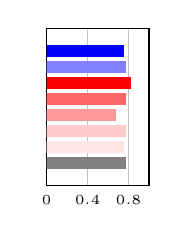
\begin{tikzpicture}

  	\begin{axis}[
   	 	xbar stacked,
		bar width=4pt,
		enlarge y limits=0.2,
    		symbolic y coords={rlstm,infers,laser,bert,qth,s2v,pms,avg},
		xmin=0,xmax=1,
  		xmajorgrids,
		tickwidth=0pt,
		xtick distance=0.40,
  		ytick=data,
		yticklabels={,,},
		scale only axis=true,
  		width=1.3cm,height=2cm,
		tick label style={font=\tiny}
  	]

		% avg
  		\addplot[blue,fill] coordinates
  			{(0.754,avg) (0.00,pms) (0.00,s2v) (0.00,qth) (0.00,bert) (0.00,laser) (0.00,infers) (0.00,rlstm)};
		% pms
		\addplot[blue!50,fill] coordinates
			{(0.00,avg) (0.771,pms) (0.00,s2v) (0.00,qth) (0.00,bert) (0.00,laser) (0.00,infers) (0.00,rlstm)};

		% s2v
		\addplot[red,fill] coordinates 
			{(0.00,avg) (0.00,pms) (0.822,s2v) (0.00,qth) (0.00,bert) (0.00,laser) (0.00,infers) (0.00,rlstm)};
		% qth
		\addplot[red!60,fill] coordinates
			{(0.00,avg) (0.00,pms) (0.00,s2v) (0.768,qth) (0.00,bert) (0.00,laser) (0.00,infers) (0.00,rlstm)};
		% bert
		\addplot[red!40,fill] coordinates
			{(0.00,avg) (0.00,pms) (0.00,s2v) (0.00,qth) (0.673,bert) (0.00,laser) (0.00,infers) (0.00,rlstm)};
		% laser
		\addplot[red!20,fill] coordinates
			{(0.00,avg) (0.00,pms) (0.00,s2v) (0.00,qth) (0.00,bert) (0.769,laser) (0.00,infers) (0.00,rlstm)};
		% infersent
		\addplot[red!10,fill] coordinates
			{(0.00,avg) (0.00,pms) (0.00,s2v) (0.00,qth) (0.00,bert) (0.00,laser) (0.753,infers) (0.00,rlstm)};

		% rand lstm
		\addplot[gray,fill] coordinates 
			{(0.00,avg) (0.00,pms) (0.00,s2v) (0.00,qth) (0.00,bert) (0.00,laser) (0.00,infers) (0.773,rlstm)};

  	\end{axis}

\end{tikzpicture}
\end{minipage}
\hfill
\begin{minipage}{0.09\textwidth}
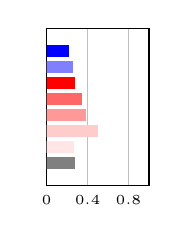
\begin{tikzpicture}

  	\begin{axis}[
    		xbar stacked,
		bar width=4pt,
		enlarge y limits=0.2,
    		symbolic y coords={rlstm,infers,laser,bert,qth,s2v,pms,avg},
		xmin=0,xmax=1,
  		xmajorgrids,
		tickwidth=0pt,
		xtick distance=0.40,
  		ytick=data,
		yticklabels={,,},
		scale only axis=true,
  		width=1.3cm,height=2cm,
		tick label style={font=\tiny}
  	]

		% avg
  		\addplot[blue,fill] coordinates
  			{(0.216,avg) (0.00,pms) (0.00,s2v) (0.00,qth) (0.00,bert) (0.00,laser) (0.00,infers) (0.00,rlstm)};
		% pms
		\addplot[blue!50,fill] coordinates
			{(0.00,avg) (0.256,pms) (0.00,s2v) (0.00,qth) (0.00,bert) (0.00,laser) (0.00,infers) (0.00,rlstm)};

		% s2v
		\addplot[red,fill] coordinates 
			{(0.00,avg) (0.00,pms) (0.269,s2v) (0.00,qth) (0.00,bert) (0.00,laser) (0.00,infers) (0.00,rlstm)};
		% qth
		\addplot[red!60,fill] coordinates
			{(0.00,avg) (0.00,pms) (0.00,s2v) (0.344,qth) (0.00,bert) (0.00,laser) (0.00,infers) (0.00,rlstm)};
		% bert
		\addplot[red!40,fill] coordinates
			{(0.00,avg) (0.00,pms) (0.00,s2v) (0.00,qth) (0.375,bert) (0.00,laser) (0.00,infers) (0.00,rlstm)};
		% laser
		\addplot[red!20,fill] coordinates
			{(0.00,avg) (0.00,pms) (0.00,s2v) (0.00,qth) (0.00,bert) (0.496,laser) (0.00,infers) (0.00,rlstm)};
		% infersent
		\addplot[red!10,fill] coordinates
			{(0.00,avg) (0.00,pms) (0.00,s2v) (0.00,qth) (0.00,bert) (0.00,laser) (0.264,infers) (0.00,rlstm)};

		% rand lstm
		\addplot[gray,fill] coordinates 
			{(0.00,avg) (0.00,pms) (0.00,s2v) (0.00,qth) (0.00,bert) (0.00,laser) (0.00,infers) (0.272,rlstm)};

  	\end{axis}

\end{tikzpicture}
\end{minipage}
%\hfill
%\begin{minipage}{0.09\textwidth}
%\begin{center}
%\textit{n.\,a.}
%\end{center}
%\end{minipage}
\hfill
\begin{minipage}{0.09\textwidth}
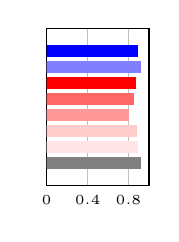
\begin{tikzpicture}

  	\begin{axis}[
    		xbar stacked,
		bar width=4pt,
		enlarge y limits=0.2,
  	  	symbolic y coords={rlstm,infers,laser,bert,qth,s2v,pms,avg},
		xmin=0,xmax=1,
  		xmajorgrids,
		tickwidth=0pt,
		xtick distance=0.40,
  		ytick=data,
		yticklabels={,,},
		scale only axis=true,
  		width=1.3cm,height=2cm,
		tick label style={font=\tiny}
  	]

		% avg
  		\addplot[blue,fill] coordinates
  			{(0.883,avg) (0.00,pms) (0.00,s2v) (0.00,qth) (0.00,bert) (0.00,laser) (0.00,infers) (0.00,rlstm)};
		% pms
		\addplot[blue!50,fill] coordinates
			{(0.00,avg) (0.912,pms) (0.00,s2v) (0.00,qth) (0.00,bert) (0.00,laser) (0.00,infers) (0.00,rlstm)};

		% s2v
		\addplot[red,fill] coordinates 
			{(0.00,avg) (0.00,pms) (0.871,s2v) (0.00,qth) (0.00,bert) (0.00,laser) (0.00,infers) (0.00,rlstm)};
		% qth
		\addplot[red!60,fill] coordinates
			{(0.00,avg) (0.00,pms) (0.00,s2v) (0.846,qth) (0.00,bert) (0.00,laser) (0.00,infers) (0.00,rlstm)};
		% bert
		\addplot[red!40,fill] coordinates
			{(0.00,avg) (0.00,pms) (0.00,s2v) (0.00,qth) (0.802,bert) (0.00,laser) (0.00,infers) (0.00,rlstm)};
		% laser
		\addplot[red!20,fill] coordinates
			{(0.00,avg) (0.00,pms) (0.00,s2v) (0.00,qth) (0.00,bert) (0.877,laser) (0.00,infers) (0.00,rlstm)};
		% infersent
		\addplot[red!10,fill] coordinates
			{(0.00,avg) (0.00,pms) (0.00,s2v) (0.00,qth) (0.00,bert) (0.00,laser) (0.891,infers) (0.00,rlstm)};

		% rand lstm
		\addplot[gray,fill] coordinates 
			{(0.00,avg) (0.00,pms) (0.00,s2v) (0.00,qth) (0.00,bert) (0.00,laser) (0.00,infers) (0.918,rlstm)};

  	\end{axis}

\end{tikzpicture}
\end{minipage}
\hfill
\begin{minipage}{0.09\textwidth}
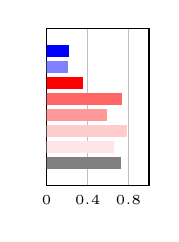
\begin{tikzpicture}

  	\begin{axis}[
   	 	xbar stacked,
		bar width=4pt,
		enlarge y limits=0.2,
   	 	symbolic y coords={rlstm,infers,laser,bert,qth,s2v,pms,avg},
		xmin=0,xmax=1,
  		xmajorgrids,
		tickwidth=0pt,
		xtick distance=0.40,
  		ytick=data,
		yticklabels={,,},
		scale only axis=true,
  		width=1.3cm,height=2cm,
		tick label style={font=\tiny}
  	]

		% avg
  		\addplot[blue,fill] coordinates
  			{(0.213,avg) (0.00,pms) (0.00,s2v) (0.00,qth) (0.00,bert) (0.00,laser) (0.00,infers) (0.00,rlstm)};
		% pms
		\addplot[blue!50,fill] coordinates
			{(0.00,avg) (0.202,pms) (0.00,s2v) (0.00,qth) (0.00,bert) (0.00,laser) (0.00,infers) (0.00,rlstm)};

		% s2v
		\addplot[red,fill] coordinates 
			{(0.00,avg) (0.00,pms) (0.351,s2v) (0.00,qth) (0.00,bert) (0.00,laser) (0.00,infers) (0.00,rlstm)};
		% qth
		\addplot[red!60,fill] coordinates
			{(0.00,avg) (0.00,pms) (0.00,s2v) (0.727,qth) (0.00,bert) (0.00,laser) (0.00,infers) (0.00,rlstm)};
		% bert
		\addplot[red!40,fill] coordinates
			{(0.00,avg) (0.00,pms) (0.00,s2v) (0.00,qth) (0.585,bert) (0.00,laser) (0.00,infers) (0.00,rlstm)};
		% laser
		\addplot[red!20,fill] coordinates
			{(0.00,avg) (0.00,pms) (0.00,s2v) (0.00,qth) (0.00,bert) (0.779,laser) (0.00,infers) (0.00,rlstm)};
		% infersent
		\addplot[red!10,fill] coordinates
			{(0.00,avg) (0.00,pms) (0.00,s2v) (0.00,qth) (0.00,bert) (0.00,laser) (0.651,infers) (0.00,rlstm)};

		% rand lstm
		\addplot[gray,fill] coordinates 
			{(0.00,avg) (0.00,pms) (0.00,s2v) (0.00,qth) (0.00,bert) (0.00,laser) (0.00,infers) (0.716,rlstm)};

  	\end{axis}

\end{tikzpicture}
\end{minipage}
\hfill
\begin{minipage}{0.09\textwidth}
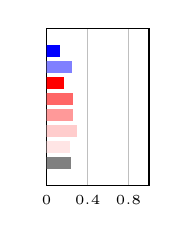
\begin{tikzpicture}

  	\begin{axis}[
   	 	xbar stacked,
		bar width=4pt,
		enlarge y limits=0.2,
    		symbolic y coords={rlstm,infers,laser,bert,qth,s2v,pms,avg},
		xmin=0,xmax=1,
  		xmajorgrids,
		tickwidth=0pt,
		xtick distance=0.40,
  		ytick=data,
		yticklabels={,,},
		scale only axis=true,
  		width=1.3cm,height=2cm,
		tick label style={font=\tiny}
  	]

		% avg
  		\addplot[blue,fill] coordinates
  			{(0.125,avg) (0.00,pms) (0.00,s2v) (0.00,qth) (0.00,bert) (0.00,laser) (0.00,infers) (0.00,rlstm)};
		% pms
		\addplot[blue!50,fill] coordinates
			{(0.00,avg) (0.239,pms) (0.00,s2v) (0.00,qth) (0.00,bert) (0.00,laser) (0.00,infers) (0.00,rlstm)};

		% s2v
		\addplot[red,fill] coordinates 
			{(0.00,avg) (0.00,pms) (0.165,s2v) (0.00,qth) (0.00,bert) (0.00,laser) (0.00,infers) (0.00,rlstm)};
		% qth
		\addplot[red!60,fill] coordinates
			{(0.00,avg) (0.00,pms) (0.00,s2v) (0.253,qth) (0.00,bert) (0.00,laser) (0.00,infers) (0.00,rlstm)};
		% bert
		\addplot[red!40,fill] coordinates
			{(0.00,avg) (0.00,pms) (0.00,s2v) (0.00,qth) (0.252,bert) (0.00,laser) (0.00,infers) (0.00,rlstm)};
		% laser
		\addplot[red!20,fill] coordinates
			{(0.00,avg) (0.00,pms) (0.00,s2v) (0.00,qth) (0.00,bert) (0.294,laser) (0.00,infers) (0.00,rlstm)};
		% infersent
		\addplot[red!10,fill] coordinates
			{(0.00,avg) (0.00,pms) (0.00,s2v) (0.00,qth) (0.00,bert) (0.00,laser) (0.225,infers) (0.00,rlstm)};

		% rand lstm
		\addplot[gray,fill] coordinates 
			{(0.00,avg) (0.00,pms) (0.00,s2v) (0.00,qth) (0.00,bert) (0.00,laser) (0.00,infers) (0.231,rlstm)};

  	\end{axis}

\end{tikzpicture}
\end{minipage}
\hfill
\begin{minipage}{0.09\textwidth}
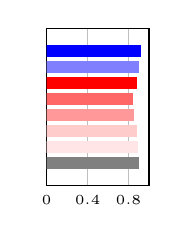
\begin{tikzpicture}

  	\begin{axis}[
 	   	xbar stacked,
		bar width=4pt,
		enlarge y limits=0.2,
   	 	symbolic y coords={rlstm,infers,laser,bert,qth,s2v,pms,avg},
		xmin=0,xmax=1,
  		xmajorgrids,
		tickwidth=0pt,
		xtick distance=0.40,
  		ytick=data,
		yticklabels={,,},
		scale only axis=true,
  		width=1.3cm,height=2cm,
		tick label style={font=\tiny}
  	]

		% avg
  		\addplot[blue,fill] coordinates
  			{(0.913,avg) (0.00,pms) (0.00,s2v) (0.00,qth) (0.00,bert) (0.00,laser) (0.00,infers) (0.00,rlstm)};
		% pms
		\addplot[blue!50,fill] coordinates
			{(0.00,avg) (0.899,pms) (0.00,s2v) (0.00,qth) (0.00,bert) (0.00,laser) (0.00,infers) (0.00,rlstm)};

		% s2v
		\addplot[red,fill] coordinates 
			{(0.00,avg) (0.00,pms) (0.876,s2v) (0.00,qth) (0.00,bert) (0.00,laser) (0.00,infers) (0.00,rlstm)};
		% qth
		\addplot[red!60,fill] coordinates
			{(0.00,avg) (0.00,pms) (0.00,s2v) (0.842,qth) (0.00,bert) (0.00,laser) (0.00,infers) (0.00,rlstm)};
		% bert
		\addplot[red!40,fill] coordinates
			{(0.00,avg) (0.00,pms) (0.00,s2v) (0.00,qth) (0.852,bert) (0.00,laser) (0.00,infers) (0.00,rlstm)};
		% laser
		\addplot[red!20,fill] coordinates
			{(0.00,avg) (0.00,pms) (0.00,s2v) (0.00,qth) (0.00,bert) (0.878,laser) (0.00,infers) (0.00,rlstm)};
		% infersent
		\addplot[red!10,fill] coordinates
			{(0.00,avg) (0.00,pms) (0.00,s2v) (0.00,qth) (0.00,bert) (0.00,laser) (0.891,infers) (0.00,rlstm)};

		% rand lstm
		\addplot[gray,fill] coordinates 
			{(0.00,avg) (0.00,pms) (0.00,s2v) (0.00,qth) (0.00,bert) (0.00,laser) (0.00,infers) (0.901,rlstm)};

  	\end{axis}

\end{tikzpicture}
\end{minipage}
\begin{center}
$\uparrow$ Russian
\end{center}
\begin{minipage}{0.115\textwidth}
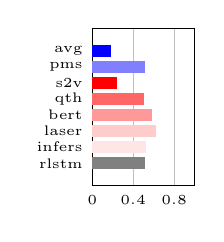
\begin{tikzpicture}

  	\begin{axis}[
    	xbar stacked,
		bar width=4pt,
		enlarge y limits=0.2,
    		symbolic y coords={rlstm,infers,laser,bert,qth,s2v,pms,avg},
		xmin=0,xmax=1,
  		xmajorgrids,
		tickwidth=0pt,
		xtick distance=0.40,
  		ytick=data,
		scale only axis=true,
  		width=1.3cm,height=2cm,
		tick label style={font=\tiny}
  	]

		% avg
  		\addplot[blue,fill] coordinates
  			{(0.174,avg) (0.00,pms) (0.00,s2v) (0.00,qth) (0.00,bert) (0.00,laser) (0.00,infers) (0.00,rlstm)};
		% pms
		\addplot[blue!50,fill] coordinates
			{(0.00,avg) (0.511,pms) (0.00,s2v) (0.00,qth) (0.00,bert) (0.00,laser) (0.00,infers) (0.00,rlstm)};

		% s2v
		\addplot[red,fill] coordinates 
			{(0.00,avg) (0.00,pms) (0.237,s2v) (0.00,qth) (0.00,bert) (0.00,laser) (0.00,infers) (0.00,rlstm)};
		% qth
		\addplot[red!60,fill] coordinates
			{(0.00,avg) (0.00,pms) (0.00,s2v) (0.504,qth) (0.00,bert) (0.00,laser) (0.00,infers) (0.00,rlstm)};
		% bert
		\addplot[red!40,fill] coordinates
			{(0.00,avg) (0.00,pms) (0.00,s2v) (0.00,qth) (0.583,bert) (0.00,laser) (0.00,infers) (0.00,rlstm)};
		% laser
		\addplot[red!20,fill] coordinates
			{(0.00,avg) (0.00,pms) (0.00,s2v) (0.00,qth) (0.00,bert) (0.615,laser) (0.00,infers) (0.00,rlstm)};
		% infersent
		\addplot[red!10,fill] coordinates
			{(0.00,avg) (0.00,pms) (0.00,s2v) (0.00,qth) (0.00,bert) (0.00,laser) (0.522,infers) (0.00,rlstm)};

		% rand lstm
		\addplot[gray,fill] coordinates 
			{(0.00,avg) (0.00,pms) (0.00,s2v) (0.00,qth) (0.00,bert) (0.00,laser) (0.00,infers) (0.514,rlstm)};

  	\end{axis}

\end{tikzpicture}
\end{minipage}
\hfill
\begin{minipage}{0.09\textwidth}
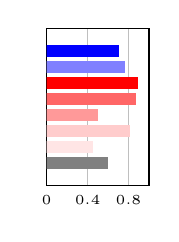
\begin{tikzpicture}

  	\begin{axis}[
    	xbar stacked,
		bar width=4pt,
		enlarge y limits=0.2,
    		symbolic y coords={rlstm,infers,laser,bert,qth,s2v,pms,avg},
		xmin=0,xmax=1,
  		xmajorgrids,
		tickwidth=0pt,
		xtick distance=0.40,
  		ytick=data,
		yticklabels={,,},
		scale only axis=true,
  		width=1.3cm,height=2cm,
		tick label style={font=\tiny}
  	]

		% avg
  		\addplot[blue,fill] coordinates
  			{(0.705,avg) (0.00,pms) (0.00,s2v) (0.00,qth) (0.00,bert) (0.00,laser) (0.00,infers) (0.00,rlstm)};
		% pms
		\addplot[blue!50,fill] coordinates
			{(0.00,avg) (0.761,pms) (0.00,s2v) (0.00,qth) (0.00,bert) (0.00,laser) (0.00,infers) (0.00,rlstm)};

		% s2v
		\addplot[red,fill] coordinates 
			{(0.00,avg) (0.00,pms) (0.891,s2v) (0.00,qth) (0.00,bert) (0.00,laser) (0.00,infers) (0.00,rlstm)};
		% qth
		\addplot[red!60,fill] coordinates
			{(0.00,avg) (0.00,pms) (0.00,s2v) (0.867,qth) (0.00,bert) (0.00,laser) (0.00,infers) (0.00,rlstm)};
		% bert
		\addplot[red!40,fill] coordinates
			{(0.00,avg) (0.00,pms) (0.00,s2v) (0.00,qth) (0.494,bert) (0.00,laser) (0.00,infers) (0.00,rlstm)};
		% laser
		\addplot[red!20,fill] coordinates
			{(0.00,avg) (0.00,pms) (0.00,s2v) (0.00,qth) (0.00,bert) (0.805,laser) (0.00,infers) (0.00,rlstm)};
		% infersent
		\addplot[red!10,fill] coordinates
			{(0.00,avg) (0.00,pms) (0.00,s2v) (0.00,qth) (0.00,bert) (0.00,laser) (0.447,infers) (0.00,rlstm)};

		% rand lstm
		\addplot[gray,fill] coordinates 
			{(0.00,avg) (0.00,pms) (0.00,s2v) (0.00,qth) (0.00,bert) (0.00,laser) (0.00,infers) (0.591,rlstm)};

  	\end{axis}

\end{tikzpicture}
\end{minipage}
\hfill
\begin{minipage}{0.09\textwidth}
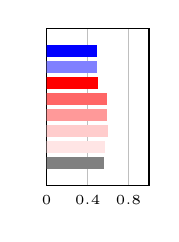
\begin{tikzpicture}

  	\begin{axis}[
    		xbar stacked,
		bar width=4pt,
		enlarge y limits=0.2,
    		symbolic y coords={rlstm,infers,laser,bert,qth,s2v,pms,avg},
		xmin=0,xmax=1,
  		xmajorgrids,
		tickwidth=0pt,
		xtick distance=0.40,
  		ytick=data,
		yticklabels={,,},
		scale only axis=true,
  		width=1.3cm,height=2cm,
		tick label style={font=\tiny}
  	]

		% avg
  		\addplot[blue,fill] coordinates
  			{(0.487,avg) (0.00,pms) (0.00,s2v) (0.00,qth) (0.00,bert) (0.00,laser) (0.00,infers) (0.00,rlstm)};
		% pms
		\addplot[blue!50,fill] coordinates
			{(0.00,avg) (0.487,pms) (0.00,s2v) (0.00,qth) (0.00,bert) (0.00,laser) (0.00,infers) (0.00,rlstm)};

		% s2v
		\addplot[red,fill] coordinates 
			{(0.00,avg) (0.00,pms) (0.493,s2v) (0.00,qth) (0.00,bert) (0.00,laser) (0.00,infers) (0.00,rlstm)};
		% qth
		\addplot[red!60,fill] coordinates
			{(0.00,avg) (0.00,pms) (0.00,s2v) (0.587,qth) (0.00,bert) (0.00,laser) (0.00,infers) (0.00,rlstm)};
		% bert
		\addplot[red!40,fill] coordinates
			{(0.00,avg) (0.00,pms) (0.00,s2v) (0.00,qth) (0.585,bert) (0.00,laser) (0.00,infers) (0.00,rlstm)};
		% laser
		\addplot[red!20,fill] coordinates
			{(0.00,avg) (0.00,pms) (0.00,s2v) (0.00,qth) (0.00,bert) (0.596,laser) (0.00,infers) (0.00,rlstm)};
		% infersent
		\addplot[red!10,fill] coordinates
			{(0.00,avg) (0.00,pms) (0.00,s2v) (0.00,qth) (0.00,bert) (0.00,laser) (0.565,infers) (0.00,rlstm)};

		% rand lstm
		\addplot[gray,fill] coordinates 
			{(0.00,avg) (0.00,pms) (0.00,s2v) (0.00,qth) (0.00,bert) (0.00,laser) (0.00,infers) (0.553,rlstm)};

  	\end{axis}

\end{tikzpicture}
\end{minipage}
\hfill
\begin{minipage}{0.09\textwidth}
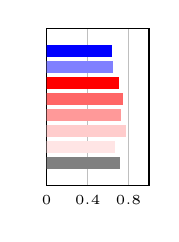
\begin{tikzpicture}

  	\begin{axis}[
   	 	xbar stacked,
		bar width=4pt,
		enlarge y limits=0.2,
    		symbolic y coords={rlstm,infers,laser,bert,qth,s2v,pms,avg},
		xmin=0,xmax=1,
  		xmajorgrids,
		tickwidth=0pt,
		xtick distance=0.40,
  		ytick=data,
		yticklabels={,,},
		scale only axis=true,
  		width=1.3cm,height=2cm,
		tick label style={font=\tiny}
  	]

		% avg
  		\addplot[blue,fill] coordinates
  			{(0.631,avg) (0.00,pms) (0.00,s2v) (0.00,qth) (0.00,bert) (0.00,laser) (0.00,infers) (0.00,rlstm)};
		% pms
		\addplot[blue!50,fill] coordinates
			{(0.00,avg) (0.642,pms) (0.00,s2v) (0.00,qth) (0.00,bert) (0.00,laser) (0.00,infers) (0.00,rlstm)};

		% s2v
		\addplot[red,fill] coordinates 
			{(0.00,avg) (0.00,pms) (0.701,s2v) (0.00,qth) (0.00,bert) (0.00,laser) (0.00,infers) (0.00,rlstm)};
		% qth
		\addplot[red!60,fill] coordinates
			{(0.00,avg) (0.00,pms) (0.00,s2v) (0.737,qth) (0.00,bert) (0.00,laser) (0.00,infers) (0.00,rlstm)};
		% bert
		\addplot[red!40,fill] coordinates
			{(0.00,avg) (0.00,pms) (0.00,s2v) (0.00,qth) (0.725,bert) (0.00,laser) (0.00,infers) (0.00,rlstm)};
		% laser
		\addplot[red!20,fill] coordinates
			{(0.00,avg) (0.00,pms) (0.00,s2v) (0.00,qth) (0.00,bert) (0.774,laser) (0.00,infers) (0.00,rlstm)};
		% infersent
		\addplot[red!10,fill] coordinates
			{(0.00,avg) (0.00,pms) (0.00,s2v) (0.00,qth) (0.00,bert) (0.00,laser) (0.658,infers) (0.00,rlstm)};

		% rand lstm
		\addplot[gray,fill] coordinates 
			{(0.00,avg) (0.00,pms) (0.00,s2v) (0.00,qth) (0.00,bert) (0.00,laser) (0.00,infers) (0.712,rlstm)};

  	\end{axis}

\end{tikzpicture}
\end{minipage}
\hfill
\begin{minipage}{0.09\textwidth}
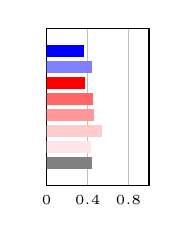
\begin{tikzpicture}

  	\begin{axis}[
    		xbar stacked,
		bar width=4pt,
		enlarge y limits=0.2,
    		symbolic y coords={rlstm,infers,laser,bert,qth,s2v,pms,avg},
		xmin=0,xmax=1,
  		xmajorgrids,
		tickwidth=0pt,
		xtick distance=0.40,
  		ytick=data,
		yticklabels={,,},
		scale only axis=true,
  		width=1.3cm,height=2cm,
		tick label style={font=\tiny}
  	]

		% avg
  		\addplot[blue,fill] coordinates
  			{(0.359,avg) (0.00,pms) (0.00,s2v) (0.00,qth) (0.00,bert) (0.00,laser) (0.00,infers) (0.00,rlstm)};
		% pms
		\addplot[blue!50,fill] coordinates
			{(0.00,avg) (0.439,pms) (0.00,s2v) (0.00,qth) (0.00,bert) (0.00,laser) (0.00,infers) (0.00,rlstm)};

		% s2v
		\addplot[red,fill] coordinates 
			{(0.00,avg) (0.00,pms) (0.367,s2v) (0.00,qth) (0.00,bert) (0.00,laser) (0.00,infers) (0.00,rlstm)};
		% qth
		\addplot[red!60,fill] coordinates
			{(0.00,avg) (0.00,pms) (0.00,s2v) (0.448,qth) (0.00,bert) (0.00,laser) (0.00,infers) (0.00,rlstm)};
		% bert
		\addplot[red!40,fill] coordinates
			{(0.00,avg) (0.00,pms) (0.00,s2v) (0.00,qth) (0.454,bert) (0.00,laser) (0.00,infers) (0.00,rlstm)};
		% laser
		\addplot[red!20,fill] coordinates
			{(0.00,avg) (0.00,pms) (0.00,s2v) (0.00,qth) (0.00,bert) (0.536,laser) (0.00,infers) (0.00,rlstm)};
		% infersent
		\addplot[red!10,fill] coordinates
			{(0.00,avg) (0.00,pms) (0.00,s2v) (0.00,qth) (0.00,bert) (0.00,laser) (0.432,infers) (0.00,rlstm)};

		% rand lstm
		\addplot[gray,fill] coordinates 
			{(0.00,avg) (0.00,pms) (0.00,s2v) (0.00,qth) (0.00,bert) (0.00,laser) (0.00,infers) (0.437,rlstm)};

  	\end{axis}

\end{tikzpicture}
\end{minipage}
%\hfill
%\begin{minipage}{0.09\textwidth}
%\begin{center}
%\textit{n.\,a.}
%\end{center}
%\end{minipage}
\hfill
\begin{minipage}{0.09\textwidth}
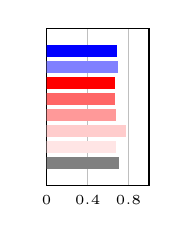
\begin{tikzpicture}

  	\begin{axis}[
    		xbar stacked,
		bar width=4pt,
		enlarge y limits=0.2,
  	  	symbolic y coords={rlstm,infers,laser,bert,qth,s2v,pms,avg},
		xmin=0,xmax=1,
  		xmajorgrids,
		tickwidth=0pt,
		xtick distance=0.40,
  		ytick=data,
		yticklabels={,,},
		scale only axis=true,
  		width=1.3cm,height=2cm,
		tick label style={font=\tiny}
  	]

		% avg
  		\addplot[blue,fill] coordinates
  			{(0.682,avg) (0.00,pms) (0.00,s2v) (0.00,qth) (0.00,bert) (0.00,laser) (0.00,infers) (0.00,rlstm)};
		% pms
		\addplot[blue!50,fill] coordinates
			{(0.00,avg) (0.690,pms) (0.00,s2v) (0.00,qth) (0.00,bert) (0.00,laser) (0.00,infers) (0.00,rlstm)};

		% s2v
		\addplot[red,fill] coordinates 
			{(0.00,avg) (0.00,pms) (0.663,s2v) (0.00,qth) (0.00,bert) (0.00,laser) (0.00,infers) (0.00,rlstm)};
		% qth
		\addplot[red!60,fill] coordinates
			{(0.00,avg) (0.00,pms) (0.00,s2v) (0.660,qth) (0.00,bert) (0.00,laser) (0.00,infers) (0.00,rlstm)};
		% bert
		\addplot[red!40,fill] coordinates
			{(0.00,avg) (0.00,pms) (0.00,s2v) (0.00,qth) (0.676,bert) (0.00,laser) (0.00,infers) (0.00,rlstm)};
		% laser
		\addplot[red!20,fill] coordinates
			{(0.00,avg) (0.00,pms) (0.00,s2v) (0.00,qth) (0.00,bert) (0.768,laser) (0.00,infers) (0.00,rlstm)};
		% infersent
		\addplot[red!10,fill] coordinates
			{(0.00,avg) (0.00,pms) (0.00,s2v) (0.00,qth) (0.00,bert) (0.00,laser) (0.670,infers) (0.00,rlstm)};

		% rand lstm
		\addplot[gray,fill] coordinates 
			{(0.00,avg) (0.00,pms) (0.00,s2v) (0.00,qth) (0.00,bert) (0.00,laser) (0.00,infers) (0.703,rlstm)};

  	\end{axis}

\end{tikzpicture}
\end{minipage}
\hfill
\begin{minipage}{0.09\textwidth}
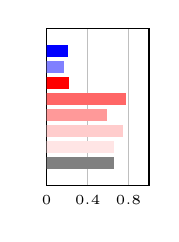
\begin{tikzpicture}

  	\begin{axis}[
   	 	xbar stacked,
		bar width=4pt,
		enlarge y limits=0.2,
   	 	symbolic y coords={rlstm,infers,laser,bert,qth,s2v,pms,avg},
		xmin=0,xmax=1,
  		xmajorgrids,
		tickwidth=0pt,
		xtick distance=0.40,
  		ytick=data,
		yticklabels={,,},
		scale only axis=true,
  		width=1.3cm,height=2cm,
		tick label style={font=\tiny}
  	]

		% avg
  		\addplot[blue,fill] coordinates
  			{(0.203,avg) (0.00,pms) (0.00,s2v) (0.00,qth) (0.00,bert) (0.00,laser) (0.00,infers) (0.00,rlstm)};
		% pms
		\addplot[blue!50,fill] coordinates
			{(0.00,avg) (0.161,pms) (0.00,s2v) (0.00,qth) (0.00,bert) (0.00,laser) (0.00,infers) (0.00,rlstm)};

		% s2v
		\addplot[red,fill] coordinates 
			{(0.00,avg) (0.00,pms) (0.210,s2v) (0.00,qth) (0.00,bert) (0.00,laser) (0.00,infers) (0.00,rlstm)};
		% qth
		\addplot[red!60,fill] coordinates
			{(0.00,avg) (0.00,pms) (0.00,s2v) (0.768,qth) (0.00,bert) (0.00,laser) (0.00,infers) (0.00,rlstm)};
		% bert
		\addplot[red!40,fill] coordinates
			{(0.00,avg) (0.00,pms) (0.00,s2v) (0.00,qth) (0.585,bert) (0.00,laser) (0.00,infers) (0.00,rlstm)};
		% laser
		\addplot[red!20,fill] coordinates
			{(0.00,avg) (0.00,pms) (0.00,s2v) (0.00,qth) (0.00,bert) (0.743,laser) (0.00,infers) (0.00,rlstm)};
		% infersent
		\addplot[red!10,fill] coordinates
			{(0.00,avg) (0.00,pms) (0.00,s2v) (0.00,qth) (0.00,bert) (0.00,laser) (0.650,infers) (0.00,rlstm)};

		% rand lstm
		\addplot[gray,fill] coordinates 
			{(0.00,avg) (0.00,pms) (0.00,s2v) (0.00,qth) (0.00,bert) (0.00,laser) (0.00,infers) (0.656,rlstm)};

  	\end{axis}

\end{tikzpicture}
\end{minipage}
\hfill
\begin{minipage}{0.09\textwidth}
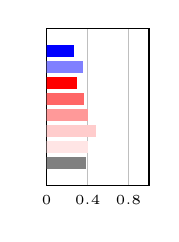
\begin{tikzpicture}

  	\begin{axis}[
   	 	xbar stacked,
		bar width=4pt,
		enlarge y limits=0.2,
    		symbolic y coords={rlstm,infers,laser,bert,qth,s2v,pms,avg},
		xmin=0,xmax=1,
  		xmajorgrids,
		tickwidth=0pt,
		xtick distance=0.40,
  		ytick=data,
		yticklabels={,,},
		scale only axis=true,
  		width=1.3cm,height=2cm,
		tick label style={font=\tiny}
  	]

		% avg
  		\addplot[blue,fill] coordinates
  			{(0.264,avg) (0.00,pms) (0.00,s2v) (0.00,qth) (0.00,bert) (0.00,laser) (0.00,infers) (0.00,rlstm)};
		% pms
		\addplot[blue!50,fill] coordinates
			{(0.00,avg) (0.353,pms) (0.00,s2v) (0.00,qth) (0.00,bert) (0.00,laser) (0.00,infers) (0.00,rlstm)};

		% s2v
		\addplot[red,fill] coordinates 
			{(0.00,avg) (0.00,pms) (0.288,s2v) (0.00,qth) (0.00,bert) (0.00,laser) (0.00,infers) (0.00,rlstm)};
		% qth
		\addplot[red!60,fill] coordinates
			{(0.00,avg) (0.00,pms) (0.00,s2v) (0.356,qth) (0.00,bert) (0.00,laser) (0.00,infers) (0.00,rlstm)};
		% bert
		\addplot[red!40,fill] coordinates
			{(0.00,avg) (0.00,pms) (0.00,s2v) (0.00,qth) (0.396,bert) (0.00,laser) (0.00,infers) (0.00,rlstm)};
		% laser
		\addplot[red!20,fill] coordinates
			{(0.00,avg) (0.00,pms) (0.00,s2v) (0.00,qth) (0.00,bert) (0.472,laser) (0.00,infers) (0.00,rlstm)};
		% infersent
		\addplot[red!10,fill] coordinates
			{(0.00,avg) (0.00,pms) (0.00,s2v) (0.00,qth) (0.00,bert) (0.00,laser) (0.398,infers) (0.00,rlstm)};

		% rand lstm
		\addplot[gray,fill] coordinates 
			{(0.00,avg) (0.00,pms) (0.00,s2v) (0.00,qth) (0.00,bert) (0.00,laser) (0.00,infers) (0.382,rlstm)};

  	\end{axis}

\end{tikzpicture}
\end{minipage}
\hfill
\begin{minipage}{0.09\textwidth}
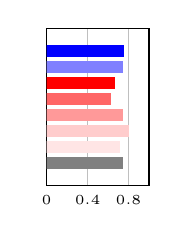
\begin{tikzpicture}

  	\begin{axis}[
 	   	xbar stacked,
		bar width=4pt,
		enlarge y limits=0.2,
   	 	symbolic y coords={rlstm,infers,laser,bert,qth,s2v,pms,avg},
		xmin=0,xmax=1,
  		xmajorgrids,
		tickwidth=0pt,
		xtick distance=0.40,
  		ytick=data,
		yticklabels={,,},
		scale only axis=true,
  		width=1.3cm,height=2cm,
		tick label style={font=\tiny}
  	]

		% avg
  		\addplot[blue,fill] coordinates
  			{(0.752,avg) (0.00,pms) (0.00,s2v) (0.00,qth) (0.00,bert) (0.00,laser) (0.00,infers) (0.00,rlstm)};
		% pms
		\addplot[blue!50,fill] coordinates
			{(0.00,avg) (0.744,pms) (0.00,s2v) (0.00,qth) (0.00,bert) (0.00,laser) (0.00,infers) (0.00,rlstm)};

		% s2v
		\addplot[red,fill] coordinates 
			{(0.00,avg) (0.00,pms) (0.663,s2v) (0.00,qth) (0.00,bert) (0.00,laser) (0.00,infers) (0.00,rlstm)};
		% qth
		\addplot[red!60,fill] coordinates
			{(0.00,avg) (0.00,pms) (0.00,s2v) (0.621,qth) (0.00,bert) (0.00,laser) (0.00,infers) (0.00,rlstm)};
		% bert
		\addplot[red!40,fill] coordinates
			{(0.00,avg) (0.00,pms) (0.00,s2v) (0.00,qth) (0.744,bert) (0.00,laser) (0.00,infers) (0.00,rlstm)};
		% laser
		\addplot[red!20,fill] coordinates
			{(0.00,avg) (0.00,pms) (0.00,s2v) (0.00,qth) (0.00,bert) (0.803,laser) (0.00,infers) (0.00,rlstm)};
		% infersent
		\addplot[red!10,fill] coordinates
			{(0.00,avg) (0.00,pms) (0.00,s2v) (0.00,qth) (0.00,bert) (0.00,laser) (0.708,infers) (0.00,rlstm)};

		% rand lstm
		\addplot[gray,fill] coordinates 
			{(0.00,avg) (0.00,pms) (0.00,s2v) (0.00,qth) (0.00,bert) (0.00,laser) (0.00,infers) (0.736,rlstm)};

  	\end{axis}

\end{tikzpicture}
\end{minipage}
\begin{center}
$\uparrow$ Turkish
\end{center}
\begin{minipage}{0.115\textwidth}
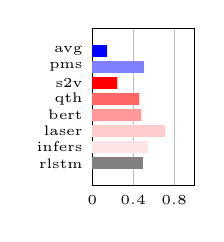
\begin{tikzpicture}

  	\begin{axis}[
    	xbar stacked,
		bar width=4pt,
		enlarge y limits=0.2,
    		symbolic y coords={rlstm,infers,laser,bert,qth,s2v,pms,avg},
		xmin=0,xmax=1,
  		xmajorgrids,
		tickwidth=0pt,
		xtick distance=0.40,
  		ytick=data,
		scale only axis=true,
  		width=1.3cm,height=2cm,
		tick label style={font=\tiny}
  	]

		% avg
  		\addplot[blue,fill] coordinates
  			{(0.140,avg) (0.00,pms) (0.00,s2v) (0.00,qth) (0.00,bert) (0.00,laser) (0.00,infers) (0.00,rlstm)};
		% pms
		\addplot[blue!50,fill] coordinates
			{(0.00,avg) (0.498,pms) (0.00,s2v) (0.00,qth) (0.00,bert) (0.00,laser) (0.00,infers) (0.00,rlstm)};

		% s2v
		\addplot[red,fill] coordinates 
			{(0.00,avg) (0.00,pms) (0.240,s2v) (0.00,qth) (0.00,bert) (0.00,laser) (0.00,infers) (0.00,rlstm)};
		% qth
		\addplot[red!60,fill] coordinates
			{(0.00,avg) (0.00,pms) (0.00,s2v) (0.454,qth) (0.00,bert) (0.00,laser) (0.00,infers) (0.00,rlstm)};
		% bert
		\addplot[red!40,fill] coordinates
			{(0.00,avg) (0.00,pms) (0.00,s2v) (0.00,qth) (0.472,bert) (0.00,laser) (0.00,infers) (0.00,rlstm)};
		% laser
		\addplot[red!20,fill] coordinates
			{(0.00,avg) (0.00,pms) (0.00,s2v) (0.00,qth) (0.00,bert) (0.705,laser) (0.00,infers) (0.00,rlstm)};
		% infersent
		\addplot[red!10,fill] coordinates
			{(0.00,avg) (0.00,pms) (0.00,s2v) (0.00,qth) (0.00,bert) (0.00,laser) (0.537,infers) (0.00,rlstm)};

		% rand lstm
		\addplot[gray,fill] coordinates 
			{(0.00,avg) (0.00,pms) (0.00,s2v) (0.00,qth) (0.00,bert) (0.00,laser) (0.00,infers) (0.487,rlstm)};

  	\end{axis}

\end{tikzpicture}
\end{minipage}
\hfill
\begin{minipage}{0.09\textwidth}
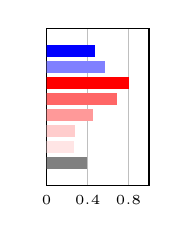
\begin{tikzpicture}

  	\begin{axis}[
    	xbar stacked,
		bar width=4pt,
		enlarge y limits=0.2,
    		symbolic y coords={rlstm,infers,laser,bert,qth,s2v,pms,avg},
		xmin=0,xmax=1,
  		xmajorgrids,
		tickwidth=0pt,
		xtick distance=0.40,
  		ytick=data,
		yticklabels={,,},
		scale only axis=true,
  		width=1.3cm,height=2cm,
		tick label style={font=\tiny}
  	]

		% avg
  		\addplot[blue,fill] coordinates
  			{(0.466,avg) (0.00,pms) (0.00,s2v) (0.00,qth) (0.00,bert) (0.00,laser) (0.00,infers) (0.00,rlstm)};
		% pms
		\addplot[blue!50,fill] coordinates
			{(0.00,avg) (0.564,pms) (0.00,s2v) (0.00,qth) (0.00,bert) (0.00,laser) (0.00,infers) (0.00,rlstm)};

		% s2v
		\addplot[red,fill] coordinates 
			{(0.00,avg) (0.00,pms) (0.799,s2v) (0.00,qth) (0.00,bert) (0.00,laser) (0.00,infers) (0.00,rlstm)};
		% qth
		\addplot[red!60,fill] coordinates
			{(0.00,avg) (0.00,pms) (0.00,s2v) (0.679,qth) (0.00,bert) (0.00,laser) (0.00,infers) (0.00,rlstm)};
		% bert
		\addplot[red!40,fill] coordinates
			{(0.00,avg) (0.00,pms) (0.00,s2v) (0.00,qth) (0.446,bert) (0.00,laser) (0.00,infers) (0.00,rlstm)};
		% laser
		\addplot[red!20,fill] coordinates
			{(0.00,avg) (0.00,pms) (0.00,s2v) (0.00,qth) (0.00,bert) (0.270,laser) (0.00,infers) (0.00,rlstm)};
		% infersent
		\addplot[red!10,fill] coordinates
			{(0.00,avg) (0.00,pms) (0.00,s2v) (0.00,qth) (0.00,bert) (0.00,laser) (0.262,infers) (0.00,rlstm)};

		% rand lstm
		\addplot[gray,fill] coordinates 
			{(0.00,avg) (0.00,pms) (0.00,s2v) (0.00,qth) (0.00,bert) (0.00,laser) (0.00,infers) (0.384,rlstm)};

  	\end{axis}

\end{tikzpicture}
\end{minipage}
\hfill
\begin{minipage}{0.09\textwidth}
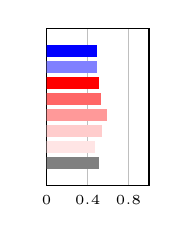
\begin{tikzpicture}

  	\begin{axis}[
    		xbar stacked,
		bar width=4pt,
		enlarge y limits=0.2,
    		symbolic y coords={rlstm,infers,laser,bert,qth,s2v,pms,avg},
		xmin=0,xmax=1,
  		xmajorgrids,
		tickwidth=0pt,
		xtick distance=0.40,
  		ytick=data,
		yticklabels={,,},
		scale only axis=true,
  		width=1.3cm,height=2cm,
		tick label style={font=\tiny}
  	]

		% avg
  		\addplot[blue,fill] coordinates
  			{(0.484,avg) (0.00,pms) (0.00,s2v) (0.00,qth) (0.00,bert) (0.00,laser) (0.00,infers) (0.00,rlstm)};
		% pms
		\addplot[blue!50,fill] coordinates
			{(0.00,avg) (0.487,pms) (0.00,s2v) (0.00,qth) (0.00,bert) (0.00,laser) (0.00,infers) (0.00,rlstm)};

		% s2v
		\addplot[red,fill] coordinates 
			{(0.00,avg) (0.00,pms) (0.501,s2v) (0.00,qth) (0.00,bert) (0.00,laser) (0.00,infers) (0.00,rlstm)};
		% qth
		\addplot[red!60,fill] coordinates
			{(0.00,avg) (0.00,pms) (0.00,s2v) (0.528,qth) (0.00,bert) (0.00,laser) (0.00,infers) (0.00,rlstm)};
		% bert
		\addplot[red!40,fill] coordinates
			{(0.00,avg) (0.00,pms) (0.00,s2v) (0.00,qth) (0.586,bert) (0.00,laser) (0.00,infers) (0.00,rlstm)};
		% laser
		\addplot[red!20,fill] coordinates
			{(0.00,avg) (0.00,pms) (0.00,s2v) (0.00,qth) (0.00,bert) (0.533,laser) (0.00,infers) (0.00,rlstm)};
		% infersent
		\addplot[red!10,fill] coordinates
			{(0.00,avg) (0.00,pms) (0.00,s2v) (0.00,qth) (0.00,bert) (0.00,laser) (0.471,infers) (0.00,rlstm)};

		% rand lstm
		\addplot[gray,fill] coordinates 
			{(0.00,avg) (0.00,pms) (0.00,s2v) (0.00,qth) (0.00,bert) (0.00,laser) (0.00,infers) (0.503,rlstm)};

  	\end{axis}

\end{tikzpicture}
\end{minipage}
\hfill
\begin{minipage}{0.09\textwidth}
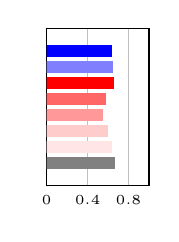
\begin{tikzpicture}

  	\begin{axis}[
   	 	xbar stacked,
		bar width=4pt,
		enlarge y limits=0.2,
    		symbolic y coords={rlstm,infers,laser,bert,qth,s2v,pms,avg},
		xmin=0,xmax=1,
  		xmajorgrids,
		tickwidth=0pt,
		xtick distance=0.40,
  		ytick=data,
		yticklabels={,,},
		scale only axis=true,
  		width=1.3cm,height=2cm,
		tick label style={font=\tiny}
  	]

		% avg
  		\addplot[blue,fill] coordinates
  			{(0.634,avg) (0.00,pms) (0.00,s2v) (0.00,qth) (0.00,bert) (0.00,laser) (0.00,infers) (0.00,rlstm)};
		% pms
		\addplot[blue!50,fill] coordinates
			{(0.00,avg) (0.639,pms) (0.00,s2v) (0.00,qth) (0.00,bert) (0.00,laser) (0.00,infers) (0.00,rlstm)};

		% s2v
		\addplot[red,fill] coordinates 
			{(0.00,avg) (0.00,pms) (0.650,s2v) (0.00,qth) (0.00,bert) (0.00,laser) (0.00,infers) (0.00,rlstm)};
		% qth
		\addplot[red!60,fill] coordinates
			{(0.00,avg) (0.00,pms) (0.00,s2v) (0.579,qth) (0.00,bert) (0.00,laser) (0.00,infers) (0.00,rlstm)};
		% bert
		\addplot[red!40,fill] coordinates
			{(0.00,avg) (0.00,pms) (0.00,s2v) (0.00,qth) (0.549,bert) (0.00,laser) (0.00,infers) (0.00,rlstm)};
		% laser
		\addplot[red!20,fill] coordinates
			{(0.00,avg) (0.00,pms) (0.00,s2v) (0.00,qth) (0.00,bert) (0.590,laser) (0.00,infers) (0.00,rlstm)};
		% infersent
		\addplot[red!10,fill] coordinates
			{(0.00,avg) (0.00,pms) (0.00,s2v) (0.00,qth) (0.00,bert) (0.00,laser) (0.635,infers) (0.00,rlstm)};

		% rand lstm
		\addplot[gray,fill] coordinates 
			{(0.00,avg) (0.00,pms) (0.00,s2v) (0.00,qth) (0.00,bert) (0.00,laser) (0.00,infers) (0.663,rlstm)};

  	\end{axis}

\end{tikzpicture}
\end{minipage}
\hfill
\begin{minipage}{0.09\textwidth}
\begin{center}
\textit{n.\,a.}
\end{center}
\end{minipage}
%\hfill
%\begin{minipage}{0.09\textwidth}
%\begin{tikzpicture}
%
%  	\begin{axis}[
%   	 	xbar stacked,
%		bar width=4pt,
%		enlarge y limits=0.2,
%    		symbolic y coords={rlstm,infers,laser,bert,qth,s2v,pms,avg},
%		xmin=0,xmax=1,
%  		xmajorgrids,
%		tickwidth=0pt,
%		xtick distance=0.40,
%  		ytick=data,
%		yticklabels={,,},
%		scale only axis=true,
%  		width=1.3cm,height=2cm,
%		tick label style={font=\tiny}
%  	]
%
%		% avg
%  		\addplot[blue,fill] coordinates
%  			{(0.08,avg) (0.00,pms) (0.00,s2v) (0.00,qth) (0.00,bert) (0.00,laser) (0.00,infers) (0.00,rlstm)};
%		% pms
%		\addplot[blue!50,fill] coordinates
%			{(0.00,avg) (0.16,pms) (0.00,s2v) (0.00,qth) (0.00,bert) (0.00,laser) (0.00,infers) (0.00,rlstm)};
%
%		% s2v
%		\addplot[red,fill] coordinates 
%			{(0.00,avg) (0.00,pms) (0.16,s2v) (0.00,qth) (0.00,bert) (0.00,laser) (0.00,infers) (0.00,rlstm)};
%		% qth
%		\addplot[red!60,fill] coordinates
%			{(0.00,avg) (0.00,pms) (0.00,s2v) (0.16,qth) (0.00,bert) (0.00,laser) (0.00,infers) (0.00,rlstm)};
%		% bert
%		\addplot[red!40,fill] coordinates
%			{(0.00,avg) (0.00,pms) (0.00,s2v) (0.00,qth) (0.17,bert) (0.00,laser) (0.00,infers) (0.00,rlstm)};
%		% laser
%		\addplot[red!20,fill] coordinates
%			{(0.00,avg) (0.00,pms) (0.00,s2v) (0.00,qth) (0.00,bert) (0.08,laser) (0.00,infers) (0.00,rlstm)};
%		% infersent
%		\addplot[red!10,fill] coordinates
%			{(0.00,avg) (0.00,pms) (0.00,s2v) (0.00,qth) (0.00,bert) (0.00,laser) (0.00,infers) (0.00,rlstm)};
%
%		% rand lstm
%		\addplot[gray,fill] coordinates 
%			{(0.00,avg) (0.00,pms) (0.00,s2v) (0.00,qth) (0.00,bert) (0.00,laser) (0.00,infers) (0.05,rlstm)};
%
%  	\end{axis}
%
%\end{tikzpicture}
%\end{minipage}
\hfill
\begin{minipage}{0.09\textwidth}
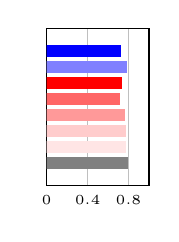
\begin{tikzpicture}

  	\begin{axis}[
    		xbar stacked,
		bar width=4pt,
		enlarge y limits=0.2,
  	  	symbolic y coords={rlstm,infers,laser,bert,qth,s2v,pms,avg},
		xmin=0,xmax=1,
  		xmajorgrids,
		tickwidth=0pt,
		xtick distance=0.40,
  		ytick=data,
		yticklabels={,,},
		scale only axis=true,
  		width=1.3cm,height=2cm,
		tick label style={font=\tiny}
  	]

		% avg
  		\addplot[blue,fill] coordinates
  			{(0.724,avg) (0.00,pms) (0.00,s2v) (0.00,qth) (0.00,bert) (0.00,laser) (0.00,infers) (0.00,rlstm)};
		% pms
		\addplot[blue!50,fill] coordinates
			{(0.00,avg) (0.782,pms) (0.00,s2v) (0.00,qth) (0.00,bert) (0.00,laser) (0.00,infers) (0.00,rlstm)};

		% s2v
		\addplot[red,fill] coordinates 
			{(0.00,avg) (0.00,pms) (0.726,s2v) (0.00,qth) (0.00,bert) (0.00,laser) (0.00,infers) (0.00,rlstm)};
		% qth
		\addplot[red!60,fill] coordinates
			{(0.00,avg) (0.00,pms) (0.00,s2v) (0.707,qth) (0.00,bert) (0.00,laser) (0.00,infers) (0.00,rlstm)};
		% bert
		\addplot[red!40,fill] coordinates
			{(0.00,avg) (0.00,pms) (0.00,s2v) (0.00,qth) (0.761,bert) (0.00,laser) (0.00,infers) (0.00,rlstm)};
		% laser
		\addplot[red!20,fill] coordinates
			{(0.00,avg) (0.00,pms) (0.00,s2v) (0.00,qth) (0.00,bert) (0.765,laser) (0.00,infers) (0.00,rlstm)};
		% infersent
		\addplot[red!10,fill] coordinates
			{(0.00,avg) (0.00,pms) (0.00,s2v) (0.00,qth) (0.00,bert) (0.00,laser) (0.771,infers) (0.00,rlstm)};

		% rand lstm
		\addplot[gray,fill] coordinates 
			{(0.00,avg) (0.00,pms) (0.00,s2v) (0.00,qth) (0.00,bert) (0.00,laser) (0.00,infers) (0.788,rlstm)};

  	\end{axis}

\end{tikzpicture}
\end{minipage}
\hfill
\begin{minipage}{0.09\textwidth}
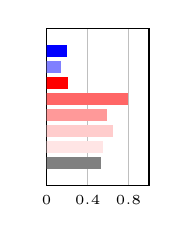
\begin{tikzpicture}

  	\begin{axis}[
   	 	xbar stacked,
		bar width=4pt,
		enlarge y limits=0.2,
   	 	symbolic y coords={rlstm,infers,laser,bert,qth,s2v,pms,avg},
		xmin=0,xmax=1,
  		xmajorgrids,
		tickwidth=0pt,
		xtick distance=0.40,
  		ytick=data,
		yticklabels={,,},
		scale only axis=true,
  		width=1.3cm,height=2cm,
		tick label style={font=\tiny}
  	]

		% avg
  		\addplot[blue,fill] coordinates
  			{(0.195,avg) (0.00,pms) (0.00,s2v) (0.00,qth) (0.00,bert) (0.00,laser) (0.00,infers) (0.00,rlstm)};
		% pms
		\addplot[blue!50,fill] coordinates
			{(0.00,avg) (0.139,pms) (0.00,s2v) (0.00,qth) (0.00,bert) (0.00,laser) (0.00,infers) (0.00,rlstm)};

		% s2v
		\addplot[red,fill] coordinates 
			{(0.00,avg) (0.00,pms) (0.206,s2v) (0.00,qth) (0.00,bert) (0.00,laser) (0.00,infers) (0.00,rlstm)};
		% qth
		\addplot[red!60,fill] coordinates
			{(0.00,avg) (0.00,pms) (0.00,s2v) (0.787,qth) (0.00,bert) (0.00,laser) (0.00,infers) (0.00,rlstm)};
		% bert
		\addplot[red!40,fill] coordinates
			{(0.00,avg) (0.00,pms) (0.00,s2v) (0.00,qth) (0.584,bert) (0.00,laser) (0.00,infers) (0.00,rlstm)};
		% laser
		\addplot[red!20,fill] coordinates
			{(0.00,avg) (0.00,pms) (0.00,s2v) (0.00,qth) (0.00,bert) (0.640,laser) (0.00,infers) (0.00,rlstm)};
		% infersent
		\addplot[red!10,fill] coordinates
			{(0.00,avg) (0.00,pms) (0.00,s2v) (0.00,qth) (0.00,bert) (0.00,laser) (0.543,infers) (0.00,rlstm)};

		% rand lstm
		\addplot[gray,fill] coordinates 
			{(0.00,avg) (0.00,pms) (0.00,s2v) (0.00,qth) (0.00,bert) (0.00,laser) (0.00,infers) (0.525,rlstm)};

  	\end{axis}

\end{tikzpicture}
\end{minipage}
\hfill
\begin{minipage}{0.09\textwidth}
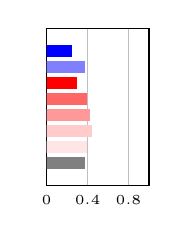
\begin{tikzpicture}

  	\begin{axis}[
   	 	xbar stacked,
		bar width=4pt,
		enlarge y limits=0.2,
    		symbolic y coords={rlstm,infers,laser,bert,qth,s2v,pms,avg},
		xmin=0,xmax=1,
  		xmajorgrids,
		tickwidth=0pt,
		xtick distance=0.40,
  		ytick=data,
		yticklabels={,,},
		scale only axis=true,
  		width=1.3cm,height=2cm,
		tick label style={font=\tiny}
  	]

		% avg
  		\addplot[blue,fill] coordinates
  			{(0.241,avg) (0.00,pms) (0.00,s2v) (0.00,qth) (0.00,bert) (0.00,laser) (0.00,infers) (0.00,rlstm)};
		% pms
		\addplot[blue!50,fill] coordinates
			{(0.00,avg) (0.366,pms) (0.00,s2v) (0.00,qth) (0.00,bert) (0.00,laser) (0.00,infers) (0.00,rlstm)};

		% s2v
		\addplot[red,fill] coordinates 
			{(0.00,avg) (0.00,pms) (0.294,s2v) (0.00,qth) (0.00,bert) (0.00,laser) (0.00,infers) (0.00,rlstm)};
		% qth
		\addplot[red!60,fill] coordinates
			{(0.00,avg) (0.00,pms) (0.00,s2v) (0.387,qth) (0.00,bert) (0.00,laser) (0.00,infers) (0.00,rlstm)};
		% bert
		\addplot[red!40,fill] coordinates
			{(0.00,avg) (0.00,pms) (0.00,s2v) (0.00,qth) (0.413,bert) (0.00,laser) (0.00,infers) (0.00,rlstm)};
		% laser
		\addplot[red!20,fill] coordinates
			{(0.00,avg) (0.00,pms) (0.00,s2v) (0.00,qth) (0.00,bert) (0.435,laser) (0.00,infers) (0.00,rlstm)};
		% infersent
		\addplot[red!10,fill] coordinates
			{(0.00,avg) (0.00,pms) (0.00,s2v) (0.00,qth) (0.00,bert) (0.00,laser) (0.393,infers) (0.00,rlstm)};

		% rand lstm
		\addplot[gray,fill] coordinates 
			{(0.00,avg) (0.00,pms) (0.00,s2v) (0.00,qth) (0.00,bert) (0.00,laser) (0.00,infers) (0.368,rlstm)};

  	\end{axis}

\end{tikzpicture}
\end{minipage}
\hfill
\begin{minipage}{0.09\textwidth}
\begin{center}
\textit{n.\,a.}
\end{center}
\end{minipage}
\begin{center}
$\uparrow$ Georgian
\end{center}
\caption[Probing task results for all languages (F1 scores)]{Probing task results for all languages (F1 scores). For reasons of legibility only the most important embeddings are shown where `avg' stands for \textit{vanilla average}, `pms' refers to the \textit{concatenated power means} embedding, `qth' is the abbreviation for \textit{Quick-Thought} and finally, `rlstm' denotes the \textit{random \gls{bilstm}}). Average embeddings were plotted using a \textcolor{blue}{blueish} color (all average methods use \textit{FastText} word embeddings) whereas trained sentence encoders are shown in a \textcolor{red}{reddish} color. The random \gls{bilstm} encoder serves as a baseline and was printed in \textcolor{gray}{gray} color. The amount of resources available decreases from top to bottom, thus, Georgian is the lowest-resource language.}
\label{fig:results_probing_tasks}
\end{figure}

% On the performance of trained encoders
\highlight{On the performance of trained encoders.} Across almost all languages it is clearly visible that \textbf{trained sentence encoders tend to work best}. \citep{Conneau.2018a} find the same pattern for the English language. The superiority of trained sentence embedding architectures is not very surprising because they learn more sophisticated operations on top of word embeddings, instead of simply computing averages. Similarly to \citep{Krasnowska.2019}, the numbers suggest that \textbf{\textit{LASER} embeddings work particularly well on many probing tasks across different languages}. Figure \vref{fig:top_three_counts} shows that for English and German, this embedding is $7\times$ among the top three of the best embeddings. For Turkish, the model even achieves top-three performance $8\times$ (with partially worse absolute scores). \citep{Krasnowska.2019} have found no concise explanation for the good performance. We believe that the main reason for this is the multi-lingual setting in which this model was trained. By exploiting similarities among languages, it is easier to produce representations of higher quality. However, the exact reasons require further investigation. \textbf{Nevertheless, this superior performance cannot be observed in the results for Georgian}: There, \textit{LASER} does not perform as convincingly as on higher-resource languages in terms of absolute scores (but remains competitive with other Georgian embeddings in terms of top-count performance as can be seen in figure \vref{fig:top_three_counts}). While the encoder may have been trained on 93 languages, the training set portion for Georgian was much smaller compared to the other languages due to the low-resource property (KA: 296k $\leftrightarrow$ DE: 8.7m). The fact that trained embeddings perform worse (measured in absolute numbers) in lower-resource languages is a general trend. As can be seen in figure \vref{fig:results_probing_tasks}, \textbf{the gap between compositional embeddings and trained sentence encoders shrinks to a great extent}: Averaging methods and random encoders occasionally surpass trained embeddings or perform on par.\footnote{An exception pose probing tasks which explicitly probe for word order information. Due to their nature, compositional models do not have knowledge about word order.} E.\,g. \textit{InferSent} sentence embeddings perform rather well on English probing tasks with a healthy gap to average embeddings, but achieve lower scores in other languages. \textbf{This decrease in performance is mainly credited to less sentence pairs available for training.} While the English model was trained on the full \textit{AllNLI} data set (\textit{SNLI} + \textit{MultiNLI}), models in low-resource languages had to resort to a reduced amount of \textit{SNLI} sentences due to the bottleneck the Google translator \gls{api} imposes. For the German model, the entire \textit{SNLI} corpus was available in advance, but the \textit{MultiNLI} data (433k sentence pairs) is missing as well.

% Figure: Top three counts
\begin{wrapfigure}{l}{0.3\textwidth}
  	\begin{center}
    		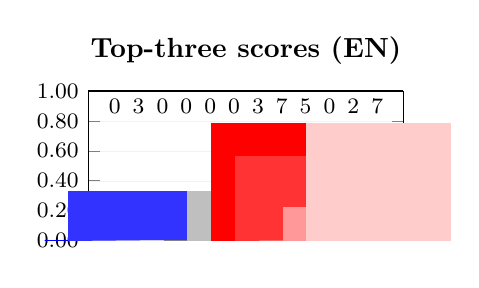
\begin{tikzpicture}[scale=1.0,every node/.style={scale=1.0}]
	\begin{axis}[
    		title=\textbf{Top-three scores (EN)},
		scale only axis,
		clip=false,
		separate axis lines,
		xtick={1,2,3,4,5,6,7,8,9,10,11,12},
        	x tick style={draw=none},
        	xticklabels={,,},
		width=4cm,height=1.9cm,
		tick label style={font=\footnotesize},
		xticklabel style={rotate=90},
		ymajorgrids,
    		grid style={line width=.1pt, draw=gray!10},
		ymin=0,ymax=1.0,
		every axis plot/.append style={
          		ybar,
          		bar width=6.0,
          		bar shift=0.5pt,
			fill
		},
		scaled y ticks=false,
		y tick label style={
        		/pgf/number format/.cd,
            		fixed,
            		fixed zerofill,
            		precision=2,
        		/tikz/.cd
    		}
	]

		\addplot[blue] coordinates {(1,0.00)};
     	 	\addplot[blue!80] coordinates {(2,0.33)};
      		\addplot[blue!60] coordinates {(3,0.00)};
      		\addplot[blue!40] coordinates {(4,0.00)};
		\addplot[blue!20] coordinates {(5,0.00)};
     	 	\addplot[gray] coordinates {(6,0.00)};
      		\addplot[lightgray] coordinates {(7,0.33)};
      		\addplot[red] coordinates {(8,0.78)};
     	 	\addplot[red!80] coordinates {(9,0.56)};
      		\addplot[red!60] coordinates {(10,0.00)};
      		\addplot[red!40] coordinates {(11,0.22)};
		\addplot[red!20] coordinates {(12,0.78)};

		\node at (axis cs: 1,0.9) {\footnotesize 0};
		\node at (axis cs: 2,0.9) {\footnotesize 3};
		\node at (axis cs: 3,0.9) {\footnotesize 0};
		\node at (axis cs: 4,0.9) {\footnotesize 0};
		\node at (axis cs: 5,0.9) {\footnotesize 0};
		\node at (axis cs: 6,0.9) {\footnotesize 0};
		\node at (axis cs: 7,0.9) {\footnotesize 3};
		\node at (axis cs: 8,0.9) {\footnotesize 7};
		\node at (axis cs: 9,0.9) {\footnotesize 5};
		\node at (axis cs: 10,0.9) {\footnotesize 0};
		\node at (axis cs: 11,0.9) {\footnotesize 2};
		\node at (axis cs: 12,0.9) {\footnotesize 7};
	\end{axis}
\end{tikzpicture}

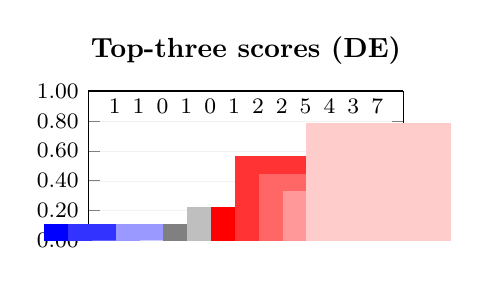
\begin{tikzpicture}[scale=1.0,every node/.style={scale=1.0}]
	\begin{axis}[
    		title=\textbf{Top-three scores (DE)},
		scale only axis,
		clip=false,
		separate axis lines,
		xtick={1,2,3,4,5,6,7,8,9,10,11,12},
        	x tick style={draw=none},
        	xticklabels={,,},
		width=4cm,height=1.9cm,
		tick label style={font=\footnotesize},
		xticklabel style={rotate=90},
		ymajorgrids,
    		grid style={line width=.1pt, draw=gray!10},
		ymin=0,ymax=1.0,
		every axis plot/.append style={
          		ybar,
          		bar width=6.0,
          		bar shift=0.5pt,
			fill
		},
		scaled y ticks=false,
		y tick label style={
        		/pgf/number format/.cd,
            		fixed,
            		fixed zerofill,
            		precision=2,
        		/tikz/.cd
    		}
	]

		\addplot[blue] coordinates {(1,0.11)};
     	 	\addplot[blue!80] coordinates {(2,0.11)};
      		\addplot[blue!60] coordinates {(3,0.00)};
      		\addplot[blue!40] coordinates {(4,0.11)};
		\addplot[blue!20] coordinates {(5,0.00)};
     	 	\addplot[gray] coordinates {(6,0.11)};
      		\addplot[lightgray] coordinates {(7,0.22)};
      		\addplot[red] coordinates {(8,0.22)};
     	 	\addplot[red!80] coordinates {(9,0.56)};
      		\addplot[red!60] coordinates {(10,0.44)};
      		\addplot[red!40] coordinates {(11,0.33)};
		\addplot[red!20] coordinates {(12,0.78)};

		\node at (axis cs: 1,0.9) {\footnotesize 1};
		\node at (axis cs: 2,0.9) {\footnotesize 1};
		\node at (axis cs: 3,0.9) {\footnotesize 0};
		\node at (axis cs: 4,0.9) {\footnotesize 1};
		\node at (axis cs: 5,0.9) {\footnotesize 0};
		\node at (axis cs: 6,0.9) {\footnotesize 1};
		\node at (axis cs: 7,0.9) {\footnotesize 2};
		\node at (axis cs: 8,0.9) {\footnotesize 2};
		\node at (axis cs: 9,0.9) {\footnotesize 5};
		\node at (axis cs: 10,0.9) {\footnotesize 4};
		\node at (axis cs: 11,0.9) {\footnotesize 3};
		\node at (axis cs: 12,0.9) {\footnotesize 7};
	\end{axis}
\end{tikzpicture}

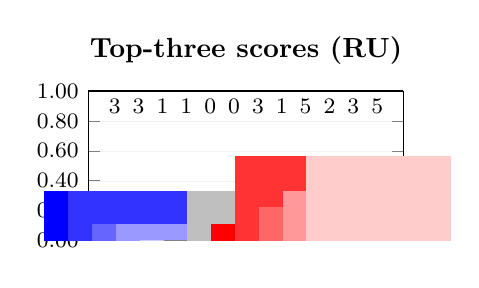
\begin{tikzpicture}[scale=1.0,every node/.style={scale=1.0}]
	\begin{axis}[
    		title=\textbf{Top-three scores (RU)},
		scale only axis,
		clip=false,
		separate axis lines,
		xtick={1,2,3,4,5,6,7,8,9,10,11,12},
        	x tick style={draw=none},
        	xticklabels={,,},
		width=4cm,height=1.9cm,
		tick label style={font=\footnotesize},
		xticklabel style={rotate=90},
		ymajorgrids,
    		grid style={line width=.1pt, draw=gray!10},
		ymin=0,ymax=1.0,
		every axis plot/.append style={
          		ybar,
          		bar width=6.0,
          		bar shift=0.5pt,
			fill
		},
		scaled y ticks=false,
		y tick label style={
        		/pgf/number format/.cd,
            		fixed,
            		fixed zerofill,
            		precision=2,
        		/tikz/.cd
    		}
	]

		\addplot[blue] coordinates {(1,0.33)};
     	 	\addplot[blue!80] coordinates {(2,0.33)};
      		\addplot[blue!60] coordinates {(3,0.11)};
      		\addplot[blue!40] coordinates {(4,0.11)};
		\addplot[blue!20] coordinates {(5,0.00)};
     	 	\addplot[gray] coordinates {(6,0.00)};
      		\addplot[lightgray] coordinates {(7,0.33)};
      		\addplot[red] coordinates {(8,0.11)};
     	 	\addplot[red!80] coordinates {(9,0.56)};
      		\addplot[red!60] coordinates {(10,0.22)};
      		\addplot[red!40] coordinates {(11,0.33)};
		\addplot[red!20] coordinates {(12,0.56)};

		\node at (axis cs: 1,0.9) {\footnotesize 3};
		\node at (axis cs: 2,0.9) {\footnotesize 3};
		\node at (axis cs: 3,0.9) {\footnotesize 1};
		\node at (axis cs: 4,0.9) {\footnotesize 1};
		\node at (axis cs: 5,0.9) {\footnotesize 0};
		\node at (axis cs: 6,0.9) {\footnotesize 0};
		\node at (axis cs: 7,0.9) {\footnotesize 3};
		\node at (axis cs: 8,0.9) {\footnotesize 1};
		\node at (axis cs: 9,0.9) {\footnotesize 5};
		\node at (axis cs: 10,0.9) {\footnotesize 2};
		\node at (axis cs: 11,0.9) {\footnotesize 3};
		\node at (axis cs: 12,0.9) {\footnotesize 5};
	\end{axis}
\end{tikzpicture}

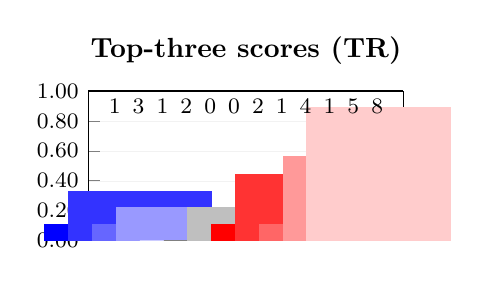
\begin{tikzpicture}[scale=1.0,every node/.style={scale=1.0}]
	\begin{axis}[
    		title=\textbf{Top-three scores (TR)},
		scale only axis,
		clip=false,
		separate axis lines,
		xtick={1,2,3,4,5,6,7,8,9,10,11,12},
        	x tick style={draw=none},
        	xticklabels={,,},
		width=4cm,height=1.9cm,
		tick label style={font=\footnotesize},
		xticklabel style={rotate=90},
		ymajorgrids,
    		grid style={line width=.1pt, draw=gray!10},
		ymin=0,ymax=1.0,
		every axis plot/.append style={
          		ybar,
          		bar width=6.0,
          		bar shift=0.5pt,
			fill
		},
		scaled y ticks=false,
		y tick label style={
        		/pgf/number format/.cd,
            		fixed,
            		fixed zerofill,
            		precision=2,
        		/tikz/.cd
    		}
	]

		\addplot[blue] coordinates {(1,0.11)};
     	 	\addplot[blue!80] coordinates {(2,0.33)};
      		\addplot[blue!60] coordinates {(3,0.11)};
      		\addplot[blue!40] coordinates {(4,0.22)};
		\addplot[blue!20] coordinates {(5,0.00)};
     	 	\addplot[gray] coordinates {(6,0.00)};
      		\addplot[lightgray] coordinates {(7,0.22)};
      		\addplot[red] coordinates {(8,0.11)};
     	 	\addplot[red!80] coordinates {(9,0.44)};
      		\addplot[red!60] coordinates {(10,0.11)};
      		\addplot[red!40] coordinates {(11,0.56)};
		\addplot[red!20] coordinates {(12,0.89)};
		
		\node at (axis cs: 1,0.9) {\footnotesize 1};
		\node at (axis cs: 2,0.9) {\footnotesize 3};
		\node at (axis cs: 3,0.9) {\footnotesize 1};
		\node at (axis cs: 4,0.9) {\footnotesize 2};
		\node at (axis cs: 5,0.9) {\footnotesize 0};
		\node at (axis cs: 6,0.9) {\footnotesize 0};
		\node at (axis cs: 7,0.9) {\footnotesize 2};
		\node at (axis cs: 8,0.9) {\footnotesize 1};
		\node at (axis cs: 9,0.9) {\footnotesize 4};
		\node at (axis cs: 10,0.9) {\footnotesize 1};
		\node at (axis cs: 11,0.9) {\footnotesize 5};
		\node at (axis cs: 12,0.9) {\footnotesize 8};
	\end{axis}
\end{tikzpicture}

\begin{tikzpicture}[scale=1.0,every node/.style={scale=1.0}]
	\begin{axis}[
    		title=\textbf{Top-three scores (KA)},
		scale only axis,
		clip=false,
		separate axis lines,
		xtick={1,2,3,4,5,6,7,8,9,10,11,12},
        	x tick style={draw=none},
        	xticklabels={Average,p-Means,SIF,GEM,Hier. pooling,BOREP,rand. BiLSTM,InferSent,Quick-Th.,sent2vec,BERT,LASER},
		width=4cm,height=1.9cm,
		tick label style={font=\footnotesize},
		xticklabel style={rotate=90},
		ymajorgrids,
    		grid style={line width=.1pt, draw=gray!10},
		ymin=0,ymax=1.0,
		every axis plot/.append style={
          		ybar,
          		bar width=6.0,
          		bar shift=0.5pt,
			fill
		},
		scaled y ticks=false,
		y tick label style={
        		/pgf/number format/.cd,
            		fixed,
            		fixed zerofill,
            		precision=2,
        		/tikz/.cd
    		}
	]

		\addplot[blue] coordinates {(1,0.00)};
     	 	\addplot[blue!80] coordinates {(2,0.57)};
      		\addplot[blue!60] coordinates {(3,0.00)};
      		\addplot[blue!40] coordinates {(4,0.00)};
		\addplot[blue!20] coordinates {(5,0.00)};
     	 	\addplot[gray] coordinates {(6,0.14)};
      		\addplot[lightgray] coordinates {(7,0.29)};
      		\addplot[red] coordinates {(8,0.43)};
     	 	\addplot[red!80] coordinates {(9,0.29)};
      		\addplot[red!60] coordinates {(10,0.29)};
      		\addplot[red!40] coordinates {(11,0.43)};
		\addplot[red!20] coordinates {(12,0.57)};

		\node at (axis cs: 1,0.9) {\footnotesize 0};
		\node at (axis cs: 2,0.9) {\footnotesize 4};
		\node at (axis cs: 3,0.9) {\footnotesize 0};
		\node at (axis cs: 4,0.9) {\footnotesize 0};
		\node at (axis cs: 5,0.9) {\footnotesize 0};
		\node at (axis cs: 6,0.9) {\footnotesize 1};
		\node at (axis cs: 7,0.9) {\footnotesize 2};
		\node at (axis cs: 8,0.9) {\footnotesize 3};
		\node at (axis cs: 9,0.9) {\footnotesize 2};
		\node at (axis cs: 10,0.9) {\footnotesize 2};
		\node at (axis cs: 11,0.9) {\footnotesize 3};
		\node at (axis cs: 12,0.9) {\footnotesize 4};
	\end{axis}
\end{tikzpicture}

  	\end{center}
  	\caption[Top-three performances for all embeddings and languages]
  	{Top-three performances for all embeddings and languages. The bar plots show scores normalized by the number of tasks.}
	\label{fig:top_three_counts}
\end{wrapfigure}

Furthermore, \textit{BERT} embeddings show mediocre performance, at least in the way they are used in this thesis. Figure \vref{fig:top_three_counts} indicates that these embeddings seem to work better in lower-resource languages, especially in Turkish ($5\times$ top-three performance). The reason for the worse top-count performance in English is that other embeddings, mainly \textit{LASER}, \textit{Quick-Thought} and \textit{InferSent}, show much stronger performance due to more training data. One further aspect contributing to the worse scores is that the embeddings were \textbf{not fine-tuned on the specific tasks which is commonly done for \textit{BERT}}. Furthermore, instead of the unusual way of using the activations of the last transformer layer, it may be worthwhile to use \textit{\gls{sbert}} \citep{Reimers.2019} or to adopt an approach similar to \citep{Krasnowska.2019} who use average \textit{BERT} embeddings. In this setup the representations are primarily seen as word embeddings which are subsequently pooled to obtain a sentence representation.

\textbf{The overall results suggest that trained encoders can still be advantageous if resources are scarce. But it may sometimes be more beneficial to rely on averaging methods rather than on trained embeddings in such a case.}

% On the performance of average methods
\highlight{On the performance of compositional methods.} Not only in lower-resource languages should the capabilities of averaging methods be underestimated. Instead, they should be considered competitive in general. It can be observed that some of the \textbf{averaging methods (especially  \textit{vanilla average} and \textit{concatenated power means} embeddings) often demonstrate surprisingly good performance on a wide range of tasks}. This has already been reported by several authors \citep[inter alia]{Arora.2017,Wieting.2016b}. Figure \vref{fig:top_three_counts} shows that they may not be among the top three as often as trained encoder architectures, but the absolute performance gap is often small. Of course, such embeddings perform randomly on tasks involving the order of words, but they excel for example in the \caps{SubjNum} task (cf. results for German, Russian and Turkish). \citep{Conneau.2018a} justify this result with \textit{`redundancies in natural language'}, i.\,e. that information about subject number is not only encoded in the subject itself, but also in other words that refer to it. For example, the form of a verb is adjusted to match the number of the subject. This means that the number information is encoded in multiple locations within a sentence. \citep{Conneau.2018a} further elaborate that word embeddings are known to retain information about tense and number \citep{Mikolov.2013c}, which is why a vector obtained by averaging these word embeddings also contains the respective information. \textbf{An additional advantage is that averages can be computed fast and efficiently.}

\textbf{On average, the choice of a specific word embedding as a basis for averaging models does not influence the results fundamentally. However, the results deviate substantially for the \caps{WC} task.} For all languages, except for German, the results suggest that, above all, the \textit{concatenated power means} embeddings exhibit much stronger performance if they are based on either \textit{word2vec} or \textit{Attract-Repel} word embeddings (cf. tables in appendix \vref{sec:appendix_probing}). Consider for example the Russian language, where the \textit{power means} embeddings achieve $\approx$ 0.99 F1 score on \caps{WC} when using \textit{word2vec} word embeddings in contrast to $\approx$ 0.67 F1 score when using \textit{FastText} vectors. For English, a similar effect can be observed: On the same task the \textit{power means} representations achieve $\approx$ 0.95 F1 score with \textit{Attract-Repel} embeddings and only $\approx$ 0.66 F1 score with \textit{FastText} embeddings. The data creation process for \caps{WC} made it necessary to increasingly resort to Wikipedia sentences. The \textit{word2vec} embeddings used in the context of this thesis were also trained on Wikipedia sentences which leads to less \gls{oov} words. Normally, \textit{FastText} can deal with words it has not seen during training by averaging $n$-gram embeddings. Unfortunately, \textbf{pre-computed word vectors were employed} without using this advantage. Therefore, the performance of \textit{FastText} is affected by more \gls{oov} words. The increased performance of \textit{Attract-Repel} must be credited to the fine-tuning of the initial vectors on linguistic constraints.

% On the universality of embeddings
\highlight{On the universality of embeddings.} Many sentence embedding techniques claim to be universal, where universality refers to the property of language representations to show strong performance, independently of the task to be solved. The design of such an embedding algorithm is a noble goal but unfortunately, \textbf{it seems that such sentence representations are not yet available}. \citep{Perone.2018} come to the same overall conclusion. The results indicate that there is no embedding that consistently shows strong performance in all probing tasks, but \textbf{\textit{LASER} can be considered closest to a universal embedding}. Nevertheless, these embeddings do not seem to capture information about subject-verb agreement well in the English language. The general lack of universality entails that there are different embeddings scoring highly on different probing tasks. Consider as an example the results generated for \textit{sent2vec}: This encoder seems to work extremely well for the detection of subject number in the German language (in this task it is the best-performing embedding with 0.906 F1 score), but the exact same algorithm performs very poorly when predicting the length of a given sentence ($\Delta$ to best-performing embedding $\approx$ 0.337 F1 score). Please note, that the ordering of the embeddings does not necessarily have to be consistent across all languages. Consider again the \caps{SubjNum} task: For German, the \textit{sent2vec} embedding performs best, while it is \textit{LASER} for the English language.

% On the performance of random encoders
\highlight{On the performance of random encoders.} \textbf{Random encoders sometimes show surprisingly strong performance}. The \textit{random \gls{bilstm}} frequently surpasses average embeddings or even trained sentence representations: In English, \textit{vanilla average} embeddings (based on \textit{FastText}) are outperformed $8\times$ and the \textit{random BiLSTM} achieves the same performance as \textit{InferSent} on the \caps{SubjNum} task. Also consider the results reported for the \caps{Voice} task in Russian: In this setting the \textit{random \gls{bilstm}} shows the best performance among all embeddings with a relative performance improvement of approximately $\Delta$ 0.006 F1 score compared to the \textit{concatenated power means} method based on \textit{FastText} word embeddings. A similar effect can be observed for the Georgian language. In Turkish, the same random encoder is at position three for the \caps{Voice} task. \citep{Wieting.2019} already pointed out that the gap between random encoders and their trained counterparts is often smaller than expected. What is more, experiments conducted by Wieting and Kiela further demonstrate that the performance is quite stable and improves with growing embedding dimensionality. \citep{Conneau.2018a} believe that a random encoder still produces a kind of \textbf{positional encoding} which can help in certain task settings.

% On the dimensionality of the embeddings
\highlight{On the dimensionality of the embeddings.} In general, one has to keep in mind that \textbf{the dimensionality of the resulting embeddings is different for almost all sentence encoding techniques}. While the majority of compositional embeddings have less dimensions (here: 300),\footnote{An exception is the \textit{p-means} technique whose dimensionality depends on the parameters. In this context it has a dimension of 1,500.} trained encoder architectures are usually high-dimensional (e.\,g. \textit{InferSent} with 4,096 dimensions). Surprisingly, we found that \textit{vanilla average} sentence embeddings occasionally perform better than the \textit{power means} approach ($1\times$ for Georgian, $2\times$ for English, German and Turkish and $3\times$ for Russian, where mostly the tasks \caps{WO} and \caps{SubjNum} are involved). Figure \vref{fig:results_probing_tasks_corr_size} generally reveals, that high dimensionality is no guarantee for good probing task performance: On the \caps{WC} task, the Pearson correlation between embedding dimensionality and performance is consistently negative across all languages. \textbf{This implies that increasing the dimensionality can sometimes hurt the performance, at least the performance as measured by the F1 score.}

\highlight{Language-specific observations.} As already mentioned above, the relative ranking of trained encoders changes in lower-resource languages. The purpose of table \vref{tab:corr_probing_lang} is to provide more information about the rank stability of the embeddings in the individual probing tasks across different languages. To this end, we computed the Spearman correlations between the probing task results in English and the remaining languages for each probing task:

% Table: Spearman correlations between languages
\begin{table}[h]
	\centering
	\renewcommand{\arraystretch}{1.3}
	\scalebox{0.90}{
	\begin{tabularx}{1.1\textwidth}{| X ? Y | Y | Y | Y | Y | Y | Y | Y | Y |}
		\hline
		\rowcolor{tud9c!50}
		\multicolumn{10}{| c |}{\textbf{Spearman correlations}}
		\\ \hline
		 &
		 \textbf{\caps{SentLen}} 	&
		 \textbf{\caps{WC}} 		&
		 \textbf{\caps{BiShift}} 	&
		 \textbf{\caps{SVAgree}} 	&
		 \textbf{\caps{SVDist}} 	&
		 \textbf{\caps{Voice}} 	&
		 \textbf{\caps{WO}} 		&
		 \textbf{\caps{EOS}} 		&
		 \textbf{\caps{SubjNum}} 	\\ \hline\hline
		\textbf{EN-DE} 	& 0.98 & 0.02 & 0.86 & 0.79 & 0.88 	&  0.34 	& 0.88 & 0.84 & -0.05 	\\ \hline
		\textbf{EN-RU} 	& 0.96 & 0.41 & 0.94 & 0.34 & 0.89 	&  0.19 	& 0.98 & 0.83 & 0.42 		\\ \hline
		\textbf{EN-TR} 	& 0.89 & 0.41 & 0.90 & 0.12 & 0.87 	& -0.06 	& 0.97 & 0.88 & 0.54 		\\ \hline
		\textbf{EN-KA} 	& 0.93 & 0.04 & 0.73 & 0.54 & - 		&  0.40 	& 0.96 & 0.89 & - 		\\ \hline
	\end{tabularx}}
	\caption[Spearman correlations between probing task performances in different languages]
		{Spearman correlations between probing task performances in different languages.}
	\label{tab:corr_probing_lang}
\end{table}

% Figure: Probing task results
\begin{figure}
\begin{minipage}{0.09\textwidth}
\begin{tikzpicture}

  	\begin{axis}[
		title=SentLen,
		enlarge y limits=0.2,
		scale only axis=true,
		xticklabels={,,},
		yticklabels={,,},
  		width=1.3cm,height=2cm,
		tickwidth=0pt,
		tick label style={font=\tiny}
  	]

		\addplot[only marks] coordinates {(4096,00.438) (8192,00.549) (300,00.240) (1500,00.553) (300,00.217) (300,00.301) (300,00.454) (4096,00.600) (2400,00.649) (700,00.254) (768,00.551) (1024,00.697)};
	
  	\end{axis}
	\node at (0.65,-0.5) {\footnotesize $r_s = 0.41$};

\end{tikzpicture}
\end{minipage}
\hfill
\begin{minipage}{0.09\textwidth}
\begin{tikzpicture}

  	\begin{axis}[
		title=WC,
   	 	enlarge y limits=0.2,
		scale only axis=true,
		xticklabels={,,},
		yticklabels={,,},
  		width=1.3cm,height=2cm,
		tickwidth=0pt,
		tick label style={font=\tiny}
  	]

		\addplot[only marks] coordinates {(4096,00.551) (8192,00.462) (300,00.581) (1500,00.657) (300,00.634) (300,00.778) (300,00.354) (4096,00.919) (2400,00.848) (700,00.786) (768,00.531) (1024,00.832)};

  	\end{axis}
	\node at (0.65,-0.5) {\footnotesize $r_s = -0.11$};

\end{tikzpicture}
\end{minipage}
\hfill
\begin{minipage}{0.09\textwidth}
\begin{tikzpicture}

  	\begin{axis}[
		title=BiShift,
 	   	enlarge y limits=0.2,
		scale only axis=true,
		xticklabels={,,},
		yticklabels={,,},
  		width=1.3cm,height=2cm,
		tickwidth=0pt,
		tick label style={font=\tiny}
  	]

		\addplot[only marks] coordinates {(4096,00.488) (8192,00.510) (300,00.485) (1500,00.491) (300,00.471) (300,00.496) (300,00.501) (4096,00.536) (2400,00.544) (700,00.534) (768,00.641) (1024,00.600)};


  	\end{axis}
	\node at (0.65,-0.5) {\footnotesize $r_s = -0.08$};

\end{tikzpicture}
\end{minipage}
\hfill
\begin{minipage}{0.09\textwidth}
\begin{tikzpicture}

  	\begin{axis}[
		title=SVAgree,
 	   	enlarge y limits=0.2,
		scale only axis=true,
		xticklabels={,,},
		yticklabels={,,},
  		width=1.3cm,height=2cm,
		tickwidth=0pt,
		tick label style={font=\tiny}
  	]

		\addplot[only marks] coordinates {(4096,00.737) (8192,00.819) (300,00.775) (1500,00.804) (300,00.808) (300,00.776) (300,00.660) (4096,00.912) (2400,00.887) (700,00.910) (768,00.718) (1024,00.572)};


  	\end{axis}
	\node at (0.65,-0.5) {\footnotesize $r_s = 0.28$};

\end{tikzpicture}
\end{minipage}
\hfill
\begin{minipage}{0.09\textwidth}
\begin{tikzpicture}

  	\begin{axis}[
		title=SVDist,
  	  	enlarge y limits=0.2,
		scale only axis=true,
		xticklabels={,,},
		yticklabels={,,},
  		width=1.3cm,height=2cm,
		tickwidth=0pt,
		tick label style={font=\tiny}
  	]

		\addplot[only marks] coordinates {(4096,00.279) (8192,00.323) (300,00.265) (1500,00.309) (300,00.256) (300,00.300) (300,00.271) (4096,00.414) (2400,00.410) (700,00.301) (768,00.406) (1024,00.521)};


  	\end{axis}
	\node at (0.65,-0.5) {\footnotesize $r_s = 0.10$};

\end{tikzpicture}
\end{minipage}
\hfill
\begin{minipage}{0.09\textwidth}
\begin{tikzpicture}

  	\begin{axis}[
		title=Voice,
    		enlarge y limits=0.2,
		scale only axis=true,
		xticklabels={,,},
		yticklabels={,,},
  		width=1.3cm,height=2cm,
		tickwidth=0pt,
		tick label style={font=\tiny}
  	]

		\addplot[only marks] coordinates {(4096,00.776) (8192,00.833) (300,00.798) (1500,00.807) (300,00.756) (300,00.718) (300,00.779) (4096,00.868) (2400,00.811) (700,00.779) (768,00.760) (1024,00.904)};


  	\end{axis}
	\node at (0.65,-0.5) {\footnotesize $r_s = 0.39$};

\end{tikzpicture}
\end{minipage}
\hfill
\begin{minipage}{0.09\textwidth}
\begin{tikzpicture}

  	\begin{axis}[
		title=WO,
   	 	enlarge y limits=0.2,
		scale only axis=true,
		xticklabels={,,},
		yticklabels={,,},
  		width=1.3cm,height=2cm,
		tickwidth=0pt,
		tick label style={font=\tiny}
  	]

		\addplot[only marks] coordinates {(4096,00.188) (8192,00.598) (300,00.201) (1500,00.173) (300,00.208) (300,00.068) (300,00.363) (4096,00.760) (2400,00.802) (700,00.381) (768,00.573) (1024,00.846)};


  	\end{axis}
	\node at (0.65,-0.5) {\footnotesize $r_s = 0.34$};

\end{tikzpicture}
\end{minipage}
\hfill
\begin{minipage}{0.09\textwidth}
\begin{tikzpicture}

  	\begin{axis}[
		title=EOS,
  	  	enlarge y limits=0.2,
		scale only axis=true,
		xticklabels={,,},
		yticklabels={,,},
  		width=1.3cm,height=2cm,
		tickwidth=0pt,
		tick label style={font=\tiny}
  	]

		\addplot[only marks] coordinates {(4096,00.213) (8192,00.246) (300,00.150) (1500,00.231) (300,00.144) (300,00.206) (300,00.232) (4096,00.230) (2400,00.221) (700,00.191) (768,00.282) (1024,00.319)};


  	\end{axis}
	\node at (0.65,-0.5) {\footnotesize $r_s = 0.22$};

\end{tikzpicture}
\end{minipage}
\hfill
\begin{minipage}{0.09\textwidth}
\begin{tikzpicture}

  	\begin{axis}[
		title=SubjNum,
    		enlarge y limits=0.2,
		scale only axis=true,
		xticklabels={,,},
		yticklabels={,,},
  		width=1.3cm,height=2cm,
		tickwidth=0pt,
		tick label style={font=\tiny}
  	]

		\addplot[only marks] coordinates {(4096,00.844) (8192,00.879) (300,00.855) (1500,00.850) (300,00.835) (300,00.797) (300,00.817) (4096,00.879) (2400,00.758) (700,00.759) (768,00.858) (1024,00.899)};


  	\end{axis}
	\node at (0.65,-0.5) {\footnotesize $r_s = 0.35$};

\end{tikzpicture}
\end{minipage}
\begin{center}
$\uparrow$ English
\end{center}
\begin{minipage}{0.09\textwidth}
\begin{tikzpicture}

  	\begin{axis}[
		enlarge y limits=0.2,
		scale only axis=true,
		xticklabels={,,},
		yticklabels={,,},
  		width=1.3cm,height=2cm,
		tickwidth=0pt,
		tick label style={font=\tiny}
  	]

		\addplot[only marks] coordinates {(4096,00.402) (8192,00.508) (300,00.195) (1500,00.492) (300,00.164) (300,00.249) (300,00.433) (4096,00.557) (2400,00.520) (700,00.271) (768,00.467) (1024,00.608)};

  	\end{axis}
	\node at (0.65,-0.5) {\footnotesize $r_s = 0.47$};

\end{tikzpicture}
\end{minipage}
\hfill
\begin{minipage}{0.09\textwidth}
\begin{tikzpicture}

  	\begin{axis}[
   	 	enlarge y limits=0.2,
		scale only axis=true,
		xticklabels={,,},
		yticklabels={,,},
  		width=1.3cm,height=2cm,
		tickwidth=0pt,
		tick label style={font=\tiny}
  	]

		\addplot[only marks] coordinates {(4096,00.668) (8192,00.577) (300,00.695) (1500,00.745) (300,00.737) (300,00.816) (300,00.524) (4096,00.449) (2400,00.346) (700,00.968) (768,00.577) (1024,00.861)};


  	\end{axis}
	\node at (0.65,-0.5) {\footnotesize $r_s = -0.39$};

\end{tikzpicture}
\end{minipage}
\hfill
\begin{minipage}{0.09\textwidth}
\begin{tikzpicture}

  	\begin{axis}[
 	   	enlarge y limits=0.2,
		scale only axis=true,
		xticklabels={,,},
		yticklabels={,,},
  		width=1.3cm,height=2cm,
		tickwidth=0pt,
		tick label style={font=\tiny}
  	]

		
		\addplot[only marks] coordinates {(4096,00.482) (8192,00.490) (300,00.489) (1500,00.489) (300,00.500) (300,00.512) (300,00.492) (4096,00.505) (2400,00.575) (700,00.521) (768,00.636) (1024,00.606)};


  	\end{axis}
	\node at (0.65,-0.5) {\footnotesize $r_s = -0.25$};

\end{tikzpicture}
\end{minipage}
\hfill
\begin{minipage}{0.09\textwidth}
\begin{tikzpicture}

  	\begin{axis}[
 	   	enlarge y limits=0.2,
		scale only axis=true,
		xticklabels={,,},
		yticklabels={,,},
  		width=1.3cm,height=2cm,
		tickwidth=0pt,
		tick label style={font=\tiny}
  	]

		\addplot[only marks] coordinates {(4096,00.846) (8192,00.847) (300,00.822) (1500,00.837) (300,00.813) (300,00.830) (300,00.794) (4096,00.834) (2400,00.825) (700,00.845) (768,00.771) (1024,00.639)};

  	\end{axis}
	\node at (0.65,-0.5) {\footnotesize $r_s = 0.32$};

\end{tikzpicture}
\end{minipage}
\hfill
\begin{minipage}{0.09\textwidth}
\begin{tikzpicture}

  	\begin{axis}[
  	  	enlarge y limits=0.2,
		scale only axis=true,
		xticklabels={,,},
		yticklabels={,,},
  		width=1.3cm,height=2cm,
		tickwidth=0pt,
		tick label style={font=\tiny}
  	]

	\addplot[only marks] coordinates {(4096,00.327) (8192,00.399) (300,00.318) (1500,00.336) (300,00.293) (300,00.325) (300,00.322) (4096,00.367) (2400,00.456) (700,00.370) (768,00.404) (1024,00.448)};

  	\end{axis}
	\node at (0.65,-0.5) {\footnotesize $r_s = 0.28$};

\end{tikzpicture}
\end{minipage}
\hfill
\begin{minipage}{0.09\textwidth}
\begin{tikzpicture}

  	\begin{axis}[
    		enlarge y limits=0.2,
		scale only axis=true,
		xticklabels={,,},
		yticklabels={,,},
  		width=1.3cm,height=2cm,
		tickwidth=0pt,
		tick label style={font=\tiny}
  	]

\addplot[only marks] coordinates {(4096,00.790) (8192,00.864) (300,00.832) (1500,00.856) (300,00.793) (300,00.854) (300,00.762) (4096,00.838) (2400,00.868) (700,00.874) (768,00.793) (1024,00.854)};


  	\end{axis}
	\node at (0.65,-0.5) {\footnotesize $r_s = 0.25$};

\end{tikzpicture}
\end{minipage}
\hfill
\begin{minipage}{0.09\textwidth}
\begin{tikzpicture}

  	\begin{axis}[
   	 	enlarge y limits=0.2,
		scale only axis=true,
		xticklabels={,,},
		yticklabels={,,},
  		width=1.3cm,height=2cm,
		tickwidth=0pt,
		tick label style={font=\tiny}
  	]

		
\addplot[only marks] coordinates {(4096,00.173) (8192,00.735) (300,00.215) (1500,00.199) (300,00.216) (300,00.222) (300,00.451) (4096,00.713) (2400,00.490) (700,00.429) (768,00.584) (1024,00.821)};


  	\end{axis}
	\node at (0.65,-0.5) {\footnotesize $r_s = 0.41$};

\end{tikzpicture}
\end{minipage}
\hfill
\begin{minipage}{0.09\textwidth}
\begin{tikzpicture}

  	\begin{axis}[
  	  	enlarge y limits=0.2,
		scale only axis=true,
		xticklabels={,,},
		yticklabels={,,},
  		width=1.3cm,height=2cm,
		tickwidth=0pt,
		tick label style={font=\tiny}
  	]

	\addplot[only marks] coordinates {(4096,00.205) (8192,00.229) (300,00.172) (1500,00.232) (300,00.153) (300,00.198) (300,00.217) (4096,00.242) (2400,00.269) (700,00.197) (768,00.269) (1024,00.307)};

  	\end{axis}
	\node at (0.65,-0.5) {\footnotesize $r_s = 0.18$};

\end{tikzpicture}
\end{minipage}
\hfill
\begin{minipage}{0.09\textwidth}
\begin{tikzpicture}

  	\begin{axis}[
    		enlarge y limits=0.2,
		scale only axis=true,
		xticklabels={,,},
		yticklabels={,,},
  		width=1.3cm,height=2cm,
		tickwidth=0pt,
		tick label style={font=\tiny}
  	]

	
\addplot[only marks] coordinates {(4096,00.858) (8192,00.895) (300,00.903) (1500,00.890) (300,00.898) (300,00.889) (300,00.833) (4096,00.882) (2400,00.901) (700,00.906) (768,00.896) (1024,00.905)};


  	\end{axis}
	\node at (0.65,-0.5) {\footnotesize $r_s = -0.05$};

\end{tikzpicture}
\end{minipage}
\begin{center}
$\uparrow$ German
\end{center}
\begin{minipage}{0.09\textwidth}
\begin{tikzpicture}

  	\begin{axis}[
		enlarge y limits=0.2,
		scale only axis=true,
		xticklabels={,,},
		yticklabels={,,},
  		width=1.3cm,height=2cm,
		tickwidth=0pt,
		tick label style={font=\tiny}
  	]

\addplot[only marks] coordinates {(4096,00.405) (8192,00.515) (300,00.208) (1500,00.519) (300,00.193) (300,00.257) (300,00.456) (4096,00.576) (2400,00.574) (700,00.273) (768,00.540) (1024,00.636)};


  	\end{axis}
	\node at (0.65,-0.5) {\footnotesize $r_s = 0.41$};

\end{tikzpicture}
\end{minipage}
\hfill
\begin{minipage}{0.09\textwidth}
\begin{tikzpicture}

  	\begin{axis}[
   	 	enlarge y limits=0.2,
		scale only axis=true,
		xticklabels={,,},
		yticklabels={,,},
  		width=1.3cm,height=2cm,
		tickwidth=0pt,
		tick label style={font=\tiny}
  	]

		\addplot[only marks] coordinates {(4096,00.515) (8192,00.552) (300,00.672) (1500,00.673) (300,00.694) (300,00.743) (300,00.443) (4096,00.389) (2400,00.904) (700,00.968) (768,00.495) (1024,00.776)};


  	\end{axis}
	\node at (0.65,-0.5) {\footnotesize $r_s = -0.34$};

\end{tikzpicture}
\end{minipage}
\hfill
\begin{minipage}{0.09\textwidth}
\begin{tikzpicture}

  	\begin{axis}[
 	   	enlarge y limits=0.2,
		scale only axis=true,
		xticklabels={,,},
		yticklabels={,,},
  		width=1.3cm,height=2cm,
		tickwidth=0pt,
		tick label style={font=\tiny}
  	]

\addplot[only marks] coordinates {(4096,00.492) (8192,00.514) (300,00.483) (1500,00.474) (300,00.494) (300,00.501) (300,00.499) (4096,00.530) (2400,00.550) (700,00.506) (768,00.597) (1024,00.574)};


  	\end{axis}
	\node at (0.65,-0.5) {\footnotesize $r_s = 0.01$};

\end{tikzpicture}
\end{minipage}
\hfill
\begin{minipage}{0.09\textwidth}
\begin{tikzpicture}

  	\begin{axis}[
 	   	enlarge y limits=0.2,
		scale only axis=true,
		xticklabels={,,},
		yticklabels={,,},
  		width=1.3cm,height=2cm,
		tickwidth=0pt,
		tick label style={font=\tiny}
  	]

\addplot[only marks] coordinates {(4096,00.752) (8192,00.773) (300,00.754) (1500,00.771) (300,00.754) (300,00.745) (300,00.707) (4096,00.753) (2400,00.768) (700,00.822) (768,00.673) (1024,00.769)};


  	\end{axis}
	\node at (0.65,-0.5) {\footnotesize $r_s = 0.21$};

\end{tikzpicture}
\end{minipage}
\hfill
\begin{minipage}{0.09\textwidth}
\begin{tikzpicture}

  	\begin{axis}[
  	  	enlarge y limits=0.2,
		scale only axis=true,
		xticklabels={,,},
		yticklabels={,,},
  		width=1.3cm,height=2cm,
		tickwidth=0pt,
		tick label style={font=\tiny}
  	]

\addplot[only marks] coordinates {(4096,00.231) (8192,00.272) (300,00.216) (1500,00.256) (300,00.213) (300,00.226) (300,00.223) (4096,00.264) (2400,00.344) (700,00.269) (768,00.375) (1024,00.496)};

  	\end{axis}
	\node at (0.65,-0.5) {\footnotesize $r_s = -0.02$};

\end{tikzpicture}
\end{minipage}
\hfill
\begin{minipage}{0.09\textwidth}
\begin{tikzpicture}

  	\begin{axis}[
    		enlarge y limits=0.2,
		scale only axis=true,
		xticklabels={,,},
		yticklabels={,,},
  		width=1.3cm,height=2cm,
		tickwidth=0pt,
		tick label style={font=\tiny}
  	]

\addplot[only marks] coordinates {(4096,00.882) (8192,00.918) (300,00.883) (1500,00.912) (300,00.848) (300,00.895) (300,00.856) (4096,00.891) (2400,00.846) (700,00.871) (768,00.802) (1024,00.877)};

  	\end{axis}
	\node at (0.65,-0.5) {\footnotesize $r_s = 0.48$};

\end{tikzpicture}
\end{minipage}
\hfill
\begin{minipage}{0.09\textwidth}
\begin{tikzpicture}

  	\begin{axis}[
   	 	enlarge y limits=0.2,
		scale only axis=true,
		xticklabels={,,},
		yticklabels={,,},
  		width=1.3cm,height=2cm,
		tickwidth=0pt,
		tick label style={font=\tiny}
  	]

	\addplot[only marks] coordinates {(4096,00.177) (8192,00.716) (300,00.213) (1500,00.202) (300,00.212) (300,00.167) (300,00.406) (4096,00.651) (2400,00.727) (700,00.351) (768,00.585) (1024,00.779)};


  	\end{axis}
	\node at (0.65,-0.5) {\footnotesize $r_s = 0.43$};

\end{tikzpicture}
\end{minipage}
\hfill
\begin{minipage}{0.09\textwidth}
\begin{tikzpicture}

  	\begin{axis}[
  	  	enlarge y limits=0.2,
		scale only axis=true,
		xticklabels={,,},
		yticklabels={,,},
  		width=1.3cm,height=2cm,
		tickwidth=0pt,
		tick label style={font=\tiny}
  	]

	
\addplot[only marks] coordinates {(4096,00.209) (8192,00.231) (300,00.125) (1500,00.239) (300,00.126) (300,00.197) (300,00.215) (4096,00.225) (2400,00.253) (700,00.165) (768,00.252) (1024,00.294)};


  	\end{axis}
	\node at (0.65,-0.5) {\footnotesize $r_s = 0.29$};

\end{tikzpicture}
\end{minipage}
\hfill
\begin{minipage}{0.09\textwidth}
\begin{tikzpicture}

  	\begin{axis}[
    		enlarge y limits=0.2,
		scale only axis=true,
		xticklabels={,,},
		yticklabels={,,},
  		width=1.3cm,height=2cm,
		tickwidth=0pt,
		tick label style={font=\tiny}
  	]

		
\addplot[only marks] coordinates {(4096,00.863) (8192,00.901) (300,00.913) (1500,00.899) (300,00.916) (300,00.876) (300,00.851) (4096,00.891) (2400,00.842) (700,00.876) (768,00.852) (1024,00.878)};


  	\end{axis}
	\node at (0.65,-0.5) {\footnotesize $r_s = 0.11$};

\end{tikzpicture}
\end{minipage}
\begin{center}
$\uparrow$ Russian
\end{center}
\begin{minipage}{0.09\textwidth}
\begin{tikzpicture}

  	\begin{axis}[
		enlarge y limits=0.2,
		scale only axis=true,
		xticklabels={,,},
		yticklabels={,,},
  		width=1.3cm,height=2cm,
		tickwidth=0pt,
		tick label style={font=\tiny}
  	]

		
\addplot[only marks] coordinates {(4096,00.407) (8192,00.514) (300,00.174) (1500,00.511) (300,00.158) (300,00.276) (300,00.419) (4096,00.522) (2400,00.504) (700,00.237) (768,00.583) (1024,00.615)};


  	\end{axis}
	\node at (0.65,-0.5) {\footnotesize $r_s = 0.41$};

\end{tikzpicture}
\end{minipage}
\hfill
\begin{minipage}{0.09\textwidth}
\begin{tikzpicture}

  	\begin{axis}[
   	 	enlarge y limits=0.2,
		scale only axis=true,
		xticklabels={,,},
		yticklabels={,,},
  		width=1.3cm,height=2cm,
		tickwidth=0pt,
		tick label style={font=\tiny}
  	]

	\addplot[only marks] coordinates {(4096,00.673) (8192,00.591) (300,00.705) (1500,00.761) (300,00.738) (300,00.798) (300,00.516) (4096,00.447) (2400,00.867) (700,00.891) (768,00.494) (1024,00.805)};
	

  	\end{axis}
	\node at (0.65,-0.5) {\footnotesize $r_s = -0.32$};

\end{tikzpicture}
\end{minipage}
\hfill
\begin{minipage}{0.09\textwidth}
\begin{tikzpicture}

  	\begin{axis}[
 	   	enlarge y limits=0.2,
		scale only axis=true,
		xticklabels={,,},
		yticklabels={,,},
  		width=1.3cm,height=2cm,
		tickwidth=0pt,
		tick label style={font=\tiny}
  	]

\addplot[only marks] coordinates {(4096,00.486) (8192,00.553) (300,00.487) (1500,00.487) (300,00.492) (300,00.503) (300,00.507) (4096,00.565) (2400,00.587) (700,00.493) (768,00.585) (1024,00.596)};

  	\end{axis}
	\node at (0.65,-0.5) {\footnotesize $r_s = 0.26$};

\end{tikzpicture}
\end{minipage}
\hfill
\begin{minipage}{0.09\textwidth}
\begin{tikzpicture}

  	\begin{axis}[
 	   	enlarge y limits=0.2,
		scale only axis=true,
		xticklabels={,,},
		yticklabels={,,},
  		width=1.3cm,height=2cm,
		tickwidth=0pt,
		tick label style={font=\tiny}
  	]

\addplot[only marks] coordinates {(4096,00.599) (8192,00.712) (300,00.631) (1500,00.642) (300,00.643) (300,00.613) (300,00.557) (4096,00.658) (2400,00.737) (700,00.701) (768,00.725) (1024,00.774)};


  	\end{axis}
	\node at (0.65,-0.5) {\footnotesize $r_s = 0.19$};

\end{tikzpicture}
\end{minipage}
\hfill
\begin{minipage}{0.09\textwidth}
\begin{tikzpicture}

  	\begin{axis}[
  	  	enlarge y limits=0.2,
		scale only axis=true,
		xticklabels={,,},
		yticklabels={,,},
  		width=1.3cm,height=2cm,
		tickwidth=0pt,
		tick label style={font=\tiny}
  	]

		
\addplot[only marks] coordinates {(4096,00.411) (8192,00.437) (300,00.359) (1500,00.439) (300,00.352) (300,00.380) (300,00.420) (4096,00.432) (2400,00.448) (700,00.367) (768,00.454) (1024,00.536)};


  	\end{axis}
	\node at (0.65,-0.5) {\footnotesize $r_s = 0.23$};

\end{tikzpicture}
\end{minipage}
\hfill
\begin{minipage}{0.09\textwidth}
\begin{tikzpicture}

  	\begin{axis}[
    		enlarge y limits=0.2,
		scale only axis=true,
		xticklabels={,,},
		yticklabels={,,},
  		width=1.3cm,height=2cm,
		tickwidth=0pt,
		tick label style={font=\tiny}
  	]


\addplot[only marks] coordinates {(4096,00.661) (8192,00.703) (300,00.682) (1500,00.690) (300,00.689) (300,00.710) (300,00.627) (4096,00.670) (2400,00.660) (700,00.663) (768,00.676) (1024,00.768)};


  	\end{axis}
	\node at (0.65,-0.5) {\footnotesize $r_s = 0.03$};

\end{tikzpicture}
\end{minipage}
\hfill
\begin{minipage}{0.09\textwidth}
\begin{tikzpicture}

  	\begin{axis}[
   	 	enlarge y limits=0.2,
		scale only axis=true,
		xticklabels={,,},
		yticklabels={,,},
  		width=1.3cm,height=2cm,
		tickwidth=0pt,
		tick label style={font=\tiny}
  	]

	
\addplot[only marks] coordinates {(4096,00.162) (8192,00.656) (300,00.203) (1500,00.161) (300,00.203) (300,00.090) (300,00.322) (4096,00.650) (2400,00.768) (700,00.210) (768,00.585) (1024,00.743)};


  	\end{axis}
	\node at (0.65,-0.5) {\footnotesize $r_s = 0.42$};

\end{tikzpicture}
\end{minipage}
\hfill
\begin{minipage}{0.09\textwidth}
\begin{tikzpicture}

  	\begin{axis}[
  	  	enlarge y limits=0.2,
		scale only axis=true,
		xticklabels={,,},
		yticklabels={,,},
  		width=1.3cm,height=2cm,
		tickwidth=0pt,
		tick label style={font=\tiny}
  	]

\addplot[only marks] coordinates {(4096,00.328) (8192,00.382) (300,00.264) (1500,00.353) (300,00.249) (300,00.305) (300,00.356) (4096,00.398) (2400,00.356) (700,00.288) (768,00.396) (1024,00.472)};

  	\end{axis}
	\node at (0.65,-0.5) {\footnotesize $r_s = 0.32$};

\end{tikzpicture}
\end{minipage}
\hfill
\begin{minipage}{0.09\textwidth}
\begin{tikzpicture}

  	\begin{axis}[
    		enlarge y limits=0.2,
		scale only axis=true,
		xticklabels={,,},
		yticklabels={,,},
  		width=1.3cm,height=2cm,
		tickwidth=0pt,
		tick label style={font=\tiny}
  	]

\addplot[only marks] coordinates {(4096,00.703) (8192,00.736) (300,00.752) (1500,00.744) (300,00.752) (300,00.759) (300,00.697) (4096,00.708) (2400,00.621) (700,00.663) (768,00.744) (1024,00.803)};


  	\end{axis}
	\node at (0.65,-0.5) {\footnotesize $r_s = -0.15$};

\end{tikzpicture}
\end{minipage}
\begin{center}
$\uparrow$ Turkish
\end{center}
\begin{minipage}{0.09\textwidth}
\begin{tikzpicture}

  	\begin{axis}[
		enlarge y limits=0.2,
		scale only axis=true,
		xticklabels={,,},
		yticklabels={,,},
  		width=1.3cm,height=2cm,
		tickwidth=0pt,
		tick label style={font=\tiny}
  	]

		
\addplot[only marks] coordinates {(4096,00.373) (8192,00.487) (300,00.140) (1500,00.498) (300,00.120) (300,00.291) (300,00.397) (4096,00.537) (2400,00.454) (700,00.240) (768,00.472) (1024,00.705)};


  	\end{axis}
	\node at (0.65,-0.5) {\footnotesize $r_s = 0.37$};

\end{tikzpicture}
\end{minipage}
\hfill
\begin{minipage}{0.09\textwidth}
\begin{tikzpicture}

  	\begin{axis}[
   	 	enlarge y limits=0.2,
		scale only axis=true,
		xticklabels={,,},
		yticklabels={,,},
  		width=1.3cm,height=2cm,
		tickwidth=0pt,
		tick label style={font=\tiny}
  	]

\addplot[only marks] coordinates {(4096,00.519) (8192,00.384) (300,00.466) (1500,00.564) (300,00.461) (300,00.704) (300,00.339) (4096,00.262) (2400,00.679) (700,00.799) (768,00.446) (1024,00.270)};
	

  	\end{axis}
	\node at (0.65,-0.5) {\footnotesize $r_s = -0.26$};

\end{tikzpicture}
\end{minipage}
\hfill
\begin{minipage}{0.09\textwidth}
\begin{tikzpicture}

  	\begin{axis}[
 	   	enlarge y limits=0.2,
		scale only axis=true,
		xticklabels={,,},
		yticklabels={,,},
  		width=1.3cm,height=2cm,
		tickwidth=0pt,
		tick label style={font=\tiny}
  	]

\addplot[only marks] coordinates {(4096,00.491) (8192,00.503) (300,00.484) (1500,00.487) (300,00.485) (300,00.491) (300,00.497) (4096,00.471) (2400,00.528) (700,00.501) (768,00.586) (1024,00.533)};
		
  	\end{axis}
	\node at (0.65,-0.5) {\footnotesize $r_s = -0.13$};

\end{tikzpicture}
\end{minipage}
\hfill
\begin{minipage}{0.09\textwidth}
\begin{tikzpicture}

  	\begin{axis}[
 	   	enlarge y limits=0.2,
		scale only axis=true,
		xticklabels={,,},
		yticklabels={,,},
  		width=1.3cm,height=2cm,
		tickwidth=0pt,
		tick label style={font=\tiny}
  	]

\addplot[only marks] coordinates {(4096,00.655) (8192,00.663) (300,00.634) (1500,00.639) (300,00.626) (300,00.630) (300,00.624) (4096,00.635) (2400,00.579) (700,00.650) (768,00.549) (1024,00.590)};
	
  	\end{axis}
	\node at (0.65,-0.5) {\footnotesize $r_s = 0.41$};

\end{tikzpicture}
\end{minipage}
\hfill
\begin{minipage}{0.09\textwidth}
\begin{center}
\textit{n.\,a.}
\end{center}
\end{minipage}
\hfill
\begin{minipage}{0.09\textwidth}
\begin{tikzpicture}

  	\begin{axis}[
    		enlarge y limits=0.2,
		scale only axis=true,
		xticklabels={,,},
		yticklabels={,,},
  		width=1.3cm,height=2cm,
		tickwidth=0pt,
		tick label style={font=\tiny}
  	]

		\addplot[only marks] coordinates {(4096,00.769) (8192,00.788) (300,00.724) (1500,00.782) (300,00.698) (300,00.755) (300,00.768) (4096,00.771) (2400,00.707) (700,00.726) (768,00.761) (1024,00.765)};

  	\end{axis}
	\node at (0.65,-0.5) {\footnotesize $r_s = 0.49$};

\end{tikzpicture}
\end{minipage}
\hfill
\begin{minipage}{0.09\textwidth}
\begin{tikzpicture}

  	\begin{axis}[
   	 	enlarge y limits=0.2,
		scale only axis=true,
		xticklabels={,,},
		yticklabels={,,},
  		width=1.3cm,height=2cm,
		tickwidth=0pt,
		tick label style={font=\tiny}
  	]

\addplot[only marks] coordinates {(4096,00.125) (8192,00.525) (300,00.195) (1500,00.139) (300,00.198) (300,00.123) (300,00.276) (4096,00.543) (2400,00.787) (700,00.206) (768,00.584) (1024,00.640)};
	
  	\end{axis}
	\node at (0.65,-0.5) {\footnotesize $r_s = 0.31$};

\end{tikzpicture}
\end{minipage}
\hfill
\begin{minipage}{0.09\textwidth}
\begin{tikzpicture}

  	\begin{axis}[
  	  	enlarge y limits=0.2,
		scale only axis=true,
		xticklabels={,,},
		yticklabels={,,},
  		width=1.3cm,height=2cm,
		tickwidth=0pt,
		tick label style={font=\tiny}
  	]

\addplot[only marks] coordinates {(4096,00.348) (8192,00.368) (300,00.241) (1500,00.366) (300,00.222) (300,00.316) (300,00.344) (4096,00.393) (2400,00.387) (700,00.294) (768,00.413) (1024,00.435)};
		


  	\end{axis}
	\node at (0.65,-0.5) {\footnotesize $r_s = 0.34$};

\end{tikzpicture}
\end{minipage}
\hfill
\begin{minipage}{0.09\textwidth}
\begin{center}
\textit{n.\,a.}
\end{center}
\end{minipage}
\begin{center}
$\uparrow$ Georgian
\end{center}
\caption[Pearson correlations of embedding performance (F1 scores) and embedding dimensionality]{Pearson correlations of embedding performance (F1 scores) and embedding dimensionality. The embedding size is plotted on the x-axis, the performance on the y-axis. The correlations imply that high dimensionality is not always a guarantee for good probing task performance.}
\label{fig:results_probing_tasks_corr_size}
\end{figure}
\newpage

For two random variables, $X$ and $Y$, the Spearman correlation is computed as follows:

\begin{align}
	r_s &= 1 - \frac{6 \cdot \sum_{i=1}^n (rank(x_i) - rank(y_i))^2}{n \cdot (n^2 - 1)}
				\qquad r_s \in [-1, 1]
\end{align}

where $n$ is the number of observations (here: the number of embeddings) and $rank(\bullet)$ outputs the rank of $\bullet$ among all observed values. The range of values a correlation coefficient can take is between -1 and 1. A positive correlation indicates that the two variables tend to increase or decrease together,\footnote{$r = +1 \equiv$ perfect positive linear correlation.} while negative values imply, that if one variable increases, the other one decreases and vice versa.\footnote{$r = -1 \equiv$ perfect negative linear correlation} If the coefficient is equal to 0, then there is no discernible (linear) correlation between the two variables \citep[pp. 135--148]{Fahrmeir.2011}.
The ordering of the embeddings in the tasks \caps{SentLen}, \caps{BiShift}, \caps{SVDist}, \caps{WO} and \caps{EOS} is rather consistent for the other languages compared to English (indicated by strong positive correlations). In contrast to this, the ordering for \caps{WC}, \caps{SVAgree}, \caps{Voice} and \caps{SubjNum} is more influenced by the underlying language (slightly negative/low positive correlations).

% Comparison of the results with the literature
\highlight{Comparison of the results with the literature.} The following paragraphs provide a comparison of the probing task results described above with those reported in the literature. The detection of possible discrepancies will stimulate further research and experiments in order to investigate their origin (cf. section \vref{sec:stability_analysis}). One has to keep in mind that we created new data sets for the probing tasks, which means that the results are not directly comparable. Nevertheless, the linguistic properties which are probed remain the same. For this reason, only strongly diverging results will be discussed and the explanations focus more on different task setups.

\ding{182} \textbf{Paper: \caps{Empirical Linguistic Study of Sentence Embeddings}.} The paper which is most similar to our work is the publication by \citep{Krasnowska.2019} who probe English and Polish sentence representations. They base their experiments on the tasks introduced by \citep{Conneau.2018a}, but modified some of them. The authors include many embedding techniques into their evaluation which are not used in this thesis. These include e.\,g. \textit{COMBO} \citep{Rybak.2018}, \textit{\gls{use}} \citep{Cer.2018} or average \textit{\gls{bert}} embeddings. The following explanations are therefore restricted to the intersecting set of embeddings (English language):

The \textit{vanilla average} representations based on \textit{FastText} perform significantly worse on \caps{SentLen} in our experiments (30.22\,\% accuracy) than reported in the literature (72.27\,\% accuracy). However, \citep{Krasnowska.2019} use a different task setup: \textbf{Their data set comprises 90k instances}, whereas we only included 10k instances at maximum due to difficulties in acquiring enough training data in lower-resource languages and we wanted the English data to be comparable. Furthermore, the authors constructed \textbf{balanced data sets}. In contrast to this, table \vref{tab:class_dist_probing_en_de} shows that the \caps{SentLen} data set follows a natural distribution in our work. The performances on the \caps{WC} task deviate in the other direction: Our experiment results in 75.92\,\% accuracy compared to 46.73\,\% accuracy reported by the authors. This can be explained by the \textbf{unequal number of classes} in the two settings: \citep{Krasnowska.2019} framed the task as a 750-way classification task, whereas there are only 30 classes considered in the present work. Classification problems usually become easier with less classes to choose from. The authors found that \textit{sent2vec} performs strongly on the \caps{WC} task. There, it shows the strongest performance among all embeddings the authors considered. We could find a similar pattern: In German and Russian, it achieves approximately 0.97 F1 score. However, it achieves rather poor scores on most of the remaining probing tasks (except for \caps{SVAgree}).

\ding{183} \textbf{Paper: \caps{What you can cram into a single \$\&!\#* Vector}.} This seminal paper by \citep{Conneau.2018a} introduces to concept of probing tasks on a large scale. The authors were the first to systematically probe sentence embeddings for different linguistic aspects using a suite of ten probing tasks. Again, the largest differences can be observed for the \caps{SentLen} task as well as the \caps{WC} task. These differences are mainly observed for the \textit{vanilla average} embeddings. The performance of \textit{InferSent}, on the other hand, is comparable. Also Conneau and colleagues use more training data. They use the \textit{SentEval} framework which includes \textbf{balanced data sets of size 120k} (100k \texttt{train}, 10k \texttt{dev}, 10k \texttt{test}). \textbf{However, the number of training examples cannot be the only difference:} A comparison of the \caps{WC} results reported by \citep{Conneau.2018a} with those by \citep{Krasnowska.2019} still reveals a large gap: \textit{Vanilla average} embeddings achieve 46.73\,\% accuracy \citep{Krasnowska.2019} while \citep{Conneau.2018a} report a score of 91.09\,\% (even though Conneau and colleagues consider 1k classes). Please note, that both authors use similar-sized training data sets. The paper by Conneau et al. reveals that they \textbf{used a logistic regression classifier instead of an \gls{mlp}}, since this produced better results for them. In contrast to this, we and \citep{Krasnowska.2019} employ an \gls{mlp}. Furthermore, \citep{Conneau.2018a} state that they \textbf{performed hyper-parameter optimization} for the following hyper-parameters: \texttt{\# hidden units} $\in \{ 50, 100, 200 \}$ and \texttt{dropout} $\in \{ 0, 0.1, 0.2 \}$). This tuning was performed on the dedicated \texttt{dev} sets of the probing tasks. In contrast, we did not conduct such a hyper-parameter tuning.

\ding{184} \textbf{Paper: \caps{Evaluation of Sentence Embeddings in Downstream and linguistic Probing Tasks}.} \citep{Perone.2018} conduct experiments which are very similar to those by \citep{Conneau.2018a}. They criticized that some state-of-the-art sentence encoders were not included in the evaluations conducted by Conneau and colleagues. The authors could show that an average of deep contextualized word embeddings is able to beat more sophisticated models trained on \gls{nli} data like \textit{InferSent}. The authors also make use of the \textit{SentEval} framework and adopted all of the probing tasks. In general, \citep{Perone.2018} report rather strong results on some of the probing tasks. Especially on \caps{WC}, Perone and colleagues get surprising outcomes: The \textit{concatenated power means} embeddings achieve 98.85\,\% accuracy on the test set, although the data set comprises 1k classes. Next to the reasons already mentioned, \textbf{a higher-dimensional sentence embedding must be held responsible}: Perone et al. use the \texttt{tf-hub} module\footnote{\url{https://github.com/UKPLab/arxiv2018-xling-sentence-embeddings} (retrieved: September 09, 2019)} which is officially provided by \citep{Rueckle.2018}. This model concatenates various power-means computed in several embedding spaces. We used one embedding space only (\textit{FastText}). Also, the authors followed the approach of \citep{Conneau.2018a} and \textbf{used a logistic regression classifier} in this task.

Furthermore, \citep{Perone.2018} state that they evaluated the sentence embeddings by \textbf{leveraging a nested cross-validation} approach for some of the downstream tasks (used for hyper-parameter optimization in the context of x-validation). However, the paper leaves it open whether they proceeded analogously for the probing tasks and also the paper does not give any indication with respect to which hyper-parameters were optimized. \textbf{We attempted to get in touch with the authors on this, but our e-mail remained unanswered.}

Finally, table \vref{tab:diff_setup} summarizes the main differences between the task setup in this work and the literature:

% Table: Different task setups
\begin{table}[h]
	\centering
	\renewcommand{\arraystretch}{1.6}
	\begin{tabularx}{\textwidth}{| X | X |}
		\hline
		\rowcolor{tud9c!50}
		\textbf{Literature} & \textbf{This work}	\\
		\hline
		$\bullet$ Monolingual or bilingual evaluation 							&
		$\bullet$ 5 languages: EN, DE, RU, TR, KA 							\\
		$\bullet$ Larger data sets (90k/120k) 								&
		$\bullet$ Data sets comprise 10k instances at maximum					\\
		$\bullet$ Balanced data sets									&
		$\bullet$ Partially imbalanced data sets							\\
		$\bullet$ Hyper-parameter optimization							&
		$\bullet$ No hyper-parameter optimization							\\
		$\bullet$ Partially different classifiers								&
		$\bullet$ Usage of an \gls{mlp} for all tasks							\\
		\hline
	\end{tabularx}
	\caption[Main setup differences for the probing tasks]{Main setup differences for the probing tasks.}
	\label{tab:diff_setup}
\end{table}

\ding{185} \caps{Probing Multilingual Sentence Representations With X-Probe}. In this paper, \citep{Ravishankar.2019} evaluate multi-lingual embeddings by aligning the sentence encoding models. As already introduced in section \vref{sec:rel_work}, the authors first train the weights of an encoder for the English language by exploiting \gls{nli} data. The sentence representations for the remaining languages are then aligned on parallel corpora by minimizing the mean squared error between the English sentence representations and the target-language representations. The resulting encoders are subsequently used and evaluated on the probing task suite introduced by \citep{Conneau.2018a}. However, the general evaluation procedure is entirely different to the approach used in this thesis. E.\,g. there are no parallel corpora in the context of the present work and also the set of encoding architectures is completely disjoint to the ones considered in this thesis. \textbf{Therefore, a direct comparison of the results does not make sense and is therefore omitted.}

% Summary
\begin{tudbox}{Summary}
\textbf{The main setup differences constitute the data set size as well as the class balance. Furthermore, many authors perform hyper-parameter optimization for the classifier architectures which was not done in this context. Also, different classifiers (e.\,g. logistic regression) are sometimes used in the literature. Section \vref{sec:stability_analysis} tries to isolate the effects of these setup choices.}
\end{tudbox}

\newpage
% -----------------------------------------------------------------------------------------------------------------------------------------------------
% Downstream application results
\subsection{Presentation of Downstream Application Results}
\label{sec:results_downstream_tasks}

Similarly to the probing tasks in the previous section, figure \vref{fig:results_downstream_tasks} illustrates the main results obtained for the downstream applications across all languages. The following paragraphs provide a description of the main observations and also compare them to results in the literature. The detailed results for the downstream tasks can be found in the appendix (cf. appendix \vref{sec:appendix_downstream}).

First of all, it is immediately apparent that \textbf{the results in downstream applications across different embedding methods are not as volatile as compared to probing task performances} (cf. figure \vref{fig:results_probing_tasks}): Simple compositional models are most of the time just behind more sophisticated methods like \textit{InferSent} or \textit{LASER} and sometimes even outperform trained encoders in low-resource languages. This narrow gap in performance suggests that the choice of a particular embedding is not as decisive in more realistic downstream applications, but it is still not completely unimportant. \citep{Perone.2018} depict similar bar plots (cf. figure \vref{fig:results_perone}, abridged) and this trend is also clearly discernible in their results (top row: probing tasks where performance is partially very different, bottom row: downstream tasks where results are more stable across the embeddings). It is not quite clear why the patterns in these two types of tasks are so different. \textbf{We assume that the artificial nature of probing tasks is responsible for the deviations.}

% Figure: Results by Perone et al.
\begin{figure}[h]
	\centering
	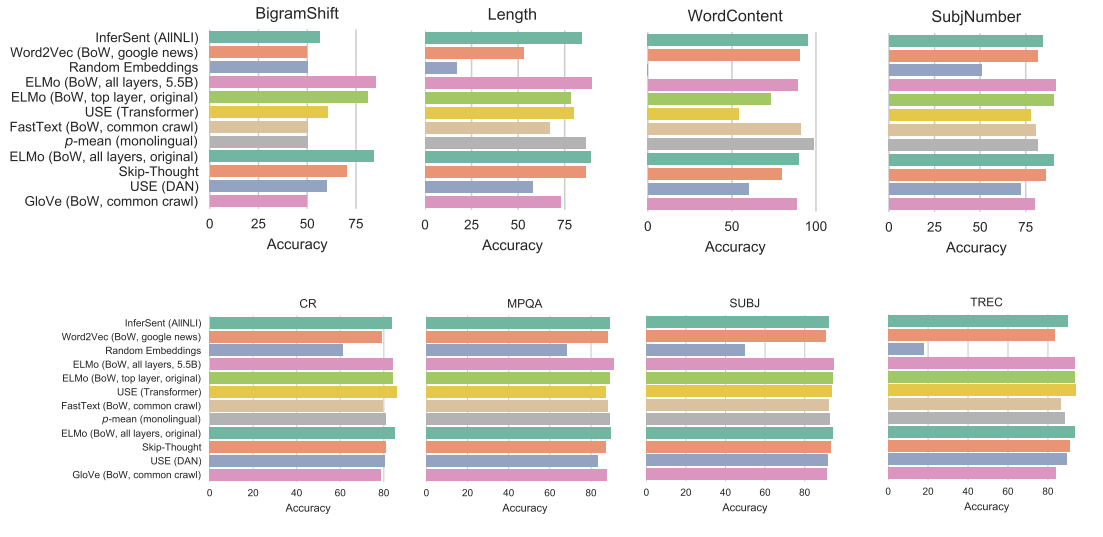
\includegraphics[scale=0.425]{images/results_perone}
	\caption[Results reported by Perone and colleagues]
		{Results for selected probing and downstream tasks as reported by \citep{Perone.2018}.}
	\label{fig:results_perone}
\end{figure}

Secondly, it is surprising that \textbf{random encoders score very highly in all languages}. The results we obtained show that such embeddings are able to outperform average embeddings (cf. \caps{TREC} task in English). \citep{Wieting.2019} find a similar pattern and therefore conclude that \textbf{random encoders \textit{`[constitute] a much stronger baseline'} than compositional models}. Comparing these results to \citep{Perone.2018} (cf. figure \vref{fig:results_perone}), one notices that they report the performance of random encoders to be substantially worse compared to the rest of the embeddings considered in their paper. Unfortunately, Perone and colleagues do not specify exactly how these embeddings were created. Differences can be caused by a different dimensionality or by a completely different encoding architecture. Despite the overall impressive performances of random encoders in this work, one can still identify a gap between those embeddings and trained sentence encoders in the English language. Nevertheless, these differences are much \textit{`smaller than [one] would have hoped'} to phrase it in the words of \citep{Wieting.2019}.

% Figure: Downstream task results
\begin{figure}
\begin{minipage}{0.265\textwidth}
\begin{tikzpicture}

  	\begin{axis}[
		title=ArgMin,
 	   	xbar stacked,
		bar width=4pt,
		enlarge y limits=0.2,
    		symbolic y coords={borep,rlstm,infers,laser,bert,qth,s2v,pms,avg},
		xmin=0,xmax=1,
  		xmajorgrids,
		tickwidth=0pt,
		xtick distance=0.40,
  		ytick=data,
		scale only axis=true,
  		width=3cm,height=2.5cm,
		tick label style={font=\tiny}
  	]

		% avg
  		\addplot[blue,fill] coordinates
  			{(0.550,avg) (0.00,pms) (0.00,s2v) (0.00,qth) (0.00,bert) (0.00,laser) (0.00,infers) (0.00,rlstm) (0.00,borep)};
		% pms
		\addplot[blue!50,fill] coordinates
			{(0.00,avg) (0.568,pms) (0.00,s2v) (0.00,qth) (0.00,bert) (0.00,laser) (0.00,infers) (0.00,rlstm) (0.00,borep)};

		% s2v
		\addplot[red,fill] coordinates 
			{(0.00,avg) (0.00,pms) (0.608,s2v) (0.00,qth) (0.00,bert) (0.00,laser) (0.00,infers) (0.00,rlstm) (0.00,borep)};
		% qth
		\addplot[red!60,fill] coordinates
			{(0.00,avg) (0.00,pms) (0.00,s2v) (0.581,qth) (0.00,bert) (0.00,laser) (0.00,infers) (0.00,rlstm) (0.00,borep)};
		% bert
		\addplot[red!40,fill] coordinates
			{(0.00,avg) (0.00,pms) (0.00,s2v) (0.00,qth) (0.558,bert) (0.00,laser) (0.00,infers) (0.00,rlstm) (0.00,borep)};
		% laser
		\addplot[red!20,fill] coordinates
			{(0.00,avg) (0.00,pms) (0.00,s2v) (0.00,qth) (0.00,bert) (0.596,laser) (0.00,infers) (0.00,rlstm) (0.00,borep)};
		% infers
		\addplot[red!10,fill] coordinates
			{(0.00,avg) (0.00,pms) (0.00,s2v) (0.00,qth) (0.00,bert) (0.00,laser) (0.604,infers) (0.00,rlstm) (0.00,borep)};

		% rand lstm
		\addplot[gray,fill] coordinates 
			{(0.00,avg) (0.00,pms) (0.00,s2v) (0.00,qth) (0.00,bert) (0.00,laser) (0.00,infers) (0.536,rlstm) (0.00,borep)};
		% borep
		\addplot[lightgray,fill] coordinates 
			{(0.00,avg) (0.00,pms) (0.00,s2v) (0.00,qth) (0.00,bert) (0.00,laser) (0.00,infers) (0.00,rlstm) (0.542,borep)};

  	\end{axis}



\end{tikzpicture}
\end{minipage}
\hfill
\begin{minipage}{0.25\textwidth}
\begin{tikzpicture}

  	\begin{axis}[
		title=Senti,
   	 	xbar stacked,
		bar width=4pt,
		enlarge y limits=0.2,
	    	symbolic y coords={borep,rlstm,infers,laser,bert,qth,s2v,pms,avg},
		xmin=0,xmax=1,
  		xmajorgrids,
		tickwidth=0pt,
		xtick distance=0.40,
  		ytick=data,
		yticklabels={,,},
		scale only axis=true,
  		width=3cm,height=2.5cm,
		tick label style={font=\tiny}
  	]

		% avg
  		\addplot[blue,fill] coordinates
  			{(0.698,avg) (0.00,pms) (0.00,s2v) (0.00,qth) (0.00,bert) (0.00,laser) (0.00,infers) (0.00,rlstm) (0.00,borep)};
		% pms
		\addplot[blue!50,fill] coordinates
			{(0.00,avg) (0.695,pms) (0.00,s2v) (0.00,qth) (0.00,bert) (0.00,laser) (0.00,infers) (0.00,rlstm) (0.00,borep)};

		% s2v
		\addplot[red,fill] coordinates 
			{(0.00,avg) (0.00,pms) (0.656,s2v) (0.00,qth) (0.00,bert) (0.00,laser) (0.00,infers) (0.00,rlstm) (0.00,borep)};
		% qth
		\addplot[red!60,fill] coordinates
			{(0.00,avg) (0.00,pms) (0.00,s2v) (0.636,qth) (0.00,bert) (0.00,laser) (0.00,infers) (0.00,rlstm) (0.00,borep)};
		% bert
		\addplot[red!40,fill] coordinates
			{(0.00,avg) (0.00,pms) (0.00,s2v) (0.00,qth) (0.644,bert) (0.00,laser) (0.00,infers) (0.00,rlstm) (0.00,borep)};
		% laser
		\addplot[red!20,fill] coordinates
			{(0.00,avg) (0.00,pms) (0.00,s2v) (0.00,qth) (0.00,bert) (0.727,laser) (0.00,infers) (0.00,rlstm) (0.00,borep)};
		% infers
		\addplot[red!10,fill] coordinates
			{(0.00,avg) (0.00,pms) (0.00,s2v) (0.00,qth) (0.00,bert) (0.00,laser) (0.702,infers) (0.00,rlstm) (0.00,borep)};

		% rand lstm
		\addplot[gray,fill] coordinates 
			{(0.00,avg) (0.00,pms) (0.00,s2v) (0.00,qth) (0.00,bert) (0.00,laser) (0.00,infers) (0.688,rlstm) (0.00,borep)};
		% borep
		\addplot[lightgray,fill] coordinates 
			{(0.00,avg) (0.00,pms) (0.00,s2v) (0.00,qth) (0.00,bert) (0.00,laser) (0.00,infers) (0.00,rlstm) (0.646,borep)};

  	\end{axis}

\end{tikzpicture}
\end{minipage}
\hfill
\begin{minipage}{0.25\textwidth}
\begin{tikzpicture}

  	\begin{axis}[
		title=TREC,
 	   	xbar stacked,
		bar width=4pt,
		enlarge y limits=0.2,
    		symbolic y coords={borep,rlstm,infers,laser,bert,qth,s2v,pms,avg},
		xmin=0,xmax=1,
  		xmajorgrids,
		tickwidth=0pt,
		xtick distance=0.40,
  		ytick=data,
		yticklabels={,,},
		scale only axis=true,
  		width=3cm,height=2.5cm,
		tick label style={font=\tiny}
  	]

		% avg
  		\addplot[blue,fill] coordinates
  			{(0.795,avg) (0.00,pms) (0.00,s2v) (0.00,qth) (0.00,bert) (0.00,laser) (0.00,infers) (0.00,rlstm) (0.00,borep)};
		% pms
		\addplot[blue!50,fill] coordinates
			{(0.00,avg) (0.767,pms) (0.00,s2v) (0.00,qth) (0.00,bert) (0.00,laser) (0.00,infers) (0.00,rlstm) (0.00,borep)};

		% s2v
		\addplot[red,fill] coordinates 
			{(0.00,avg) (0.00,pms) (0.792,s2v) (0.00,qth) (0.00,bert) (0.00,laser) (0.00,infers) (0.00,rlstm) (0.00,borep)};
		% qth
		\addplot[red!60,fill] coordinates
			{(0.00,avg) (0.00,pms) (0.00,s2v) (0.814,qth) (0.00,bert) (0.00,laser) (0.00,infers) (0.00,rlstm) (0.00,borep)};
		% bert
		\addplot[red!40,fill] coordinates
			{(0.00,avg) (0.00,pms) (0.00,s2v) (0.00,qth) (0.876,bert) (0.00,laser) (0.00,infers) (0.00,rlstm) (0.00,borep)};
		% laser
		\addplot[red!20,fill] coordinates
			{(0.00,avg) (0.00,pms) (0.00,s2v) (0.00,qth) (0.00,bert) (0.851,laser) (0.00,infers) (0.00,rlstm) (0.00,borep)};
		% infers
		\addplot[red!10,fill] coordinates
			{(0.00,avg) (0.00,pms) (0.00,s2v) (0.00,qth) (0.00,bert) (0.00,laser) (0.920,infers) (0.00,rlstm) (0.00,borep)};

		% rand lstm
		\addplot[gray,fill] coordinates 
			{(0.00,avg) (0.00,pms) (0.00,s2v) (0.00,qth) (0.00,bert) (0.00,laser) (0.00,infers) (0.774,rlstm) (0.00,borep)};
		% borep
		\addplot[lightgray,fill] coordinates 
			{(0.00,avg) (0.00,pms) (0.00,s2v) (0.00,qth) (0.00,bert) (0.00,laser) (0.00,infers) (0.00,rlstm) (0.819,borep)};

  	\end{axis}

\end{tikzpicture}
\end{minipage}
%\hfill
%\begin{minipage}{0.2\textwidth}
%\begin{tikzpicture}
%
%  	\begin{axis}[
%		title=SUBJ,
% 	   	xbar stacked,
%		bar width=4pt,
%		enlarge y limits=0.2,
%    		symbolic y coords={rlstm,infers,laser,bert,qth,s2v,pms,avg},
%		xmin=0,xmax=1,
%  		xmajorgrids,
%		tickwidth=0pt,
%		xtick distance=0.40,
%  		ytick=data,
%		yticklabels={,,},
%		scale only axis=true,
%  		width=3cm,height=2cm,
%		tick label style={font=\tiny}
%  	]
%
%		% avg
%  		\addplot[blue,fill] coordinates
%  			{(0.908,avg) (0.00,pms) (0.00,s2v) (0.00,qth) (0.00,bert) (0.00,laser) (0.00,infers) (0.00,rlstm)};
%		% pms
%		\addplot[blue!50,fill] coordinates
%			{(0.00,avg) (0.896,pms) (0.00,s2v) (0.00,qth) (0.00,bert) (0.00,laser) (0.00,infers) (0.00,rlstm)};
%
%		% s2v
%		\addplot[red,fill] coordinates 
%			{(0.00,avg) (0.00,pms) (0.920,s2v) (0.00,qth) (0.00,bert) (0.00,laser) (0.00,infers) (0.00,rlstm)};
%		% qth
%		\addplot[red!60,fill] coordinates
%			{(0.00,avg) (0.00,pms) (0.00,s2v) (0.816,qth) (0.00,bert) (0.00,laser) (0.00,infers) (0.00,rlstm)};
%		% bert
%		\addplot[red!40,fill] coordinates
%			{(0.00,avg) (0.00,pms) (0.00,s2v) (0.00,qth) (0.928,bert) (0.00,laser) (0.00,infers) (0.00,rlstm)};
%		% laser
%		\addplot[red!20,fill] coordinates
%			{(0.00,avg) (0.00,pms) (0.00,s2v) (0.00,qth) (0.00,bert) (0.914,laser) (0.00,infers) (0.00,rlstm)};
%		% infers
%		\addplot[red!20,fill] coordinates
%			{(0.00,avg) (0.00,pms) (0.00,s2v) (0.00,qth) (0.00,bert) (0.00,laser) (0.912,infers) (0.00,rlstm)};
%
%		% rand lstm
%		\addplot[gray,fill] coordinates 
%			{(0.00,avg) (0.00,pms) (0.00,s2v) (0.00,qth) (0.00,bert) (0.00,laser) (0.00,infers) (0.903,rlstm)};
%
%  	\end{axis}
%
%\end{tikzpicture}
%\end{minipage}
%\hfill
%\begin{minipage}{0.1\textwidth}
%\begin{tikzpicture}
%
%  	\begin{axis}[
%		title=Cluster,
%   	 	xbar stacked,
%		bar width=4pt,
%		enlarge y limits=0.2,
%	    	symbolic y coords={rlstm,infers,laser,bert,qth,s2v,pms,avg},
%		xmin=0,xmax=1,
%  		xmajorgrids,
%		tickwidth=0pt,
%		xtick distance=0.40,
%  		ytick=data,
%		yticklabels={,,},
%		scale only axis=true,
%  		width=1.3cm,height=2cm,
%		tick label style={font=\tiny}
%  	]
%
%		% avg
%  		\addplot[blue,fill] coordinates
%  			{(0.00,avg) (0.00,pms) (0.00,s2v) (0.00,qth) (0.00,bert) (0.00,laser) (0.00,infers) (0.00,rlstm)};
%		% pms
%		\addplot[blue!50,fill] coordinates
%			{(0.00,avg) (0.00,pms) (0.00,s2v) (0.00,qth) (0.00,bert) (0.00,laser) (0.00,infers) (0.00,rlstm)};
%
%		% s2v
%		\addplot[red,fill] coordinates 
%			{(0.00,avg) (0.00,pms) (0.00,s2v) (0.00,qth) (0.00,bert) (0.00,laser) (0.00,infers) (0.00,rlstm)};
%		% qth
%		\addplot[red!60,fill] coordinates
%			{(0.00,avg) (0.00,pms) (0.00,s2v) (0.00,qth) (0.00,bert) (0.00,laser) (0.00,infers) (0.00,rlstm)};
%		% bert
%		\addplot[red!40,fill] coordinates
%			{(0.00,avg) (0.00,pms) (0.00,s2v) (0.00,qth) (0.00,bert) (0.00,laser) (0.00,infers) (0.00,rlstm)};
%		% laser
%		\addplot[red!20,fill] coordinates
%			{(0.00,avg) (0.00,pms) (0.00,s2v) (0.00,qth) (0.00,bert) (0.00,laser) (0.00,infers) (0.00,rlstm)};
%		% infers
%		\addplot[red!20,fill] coordinates
%			{(0.00,avg) (0.00,pms) (0.00,s2v) (0.00,qth) (0.00,bert) (0.00,laser) (0.00,infers) (0.00,rlstm)};
%
%		% rand lstm
%		\addplot[gray,fill] coordinates 
%			{(0.00,avg) (0.00,pms) (0.00,s2v) (0.00,qth) (0.00,bert) (0.00,laser) (0.00,infers) (0.00,rlstm)};
%
%  	\end{axis}
%
%\end{tikzpicture}
%\end{minipage}
%\hfill
%\begin{minipage}{0.1\textwidth}
%\begin{tikzpicture}
%
%  	\begin{axis}[
%		title=MR,
%    		xbar stacked,
%		bar width=4pt,
%		enlarge y limits=0.2,
%    		symbolic y coords={rlstm,infers,laser,bert,qth,s2v,pms,avg},
%		xmin=0,xmax=1,
%  		xmajorgrids,
%		tickwidth=0pt,
%		xtick distance=0.40,
%  		ytick=data,
%		yticklabels={,,},
%		scale only axis=true,
%  		width=1.3cm,height=2cm,
%		tick label style={font=\tiny}
%  	]
%
%		% avg
%  		\addplot[blue,fill] coordinates
%  			{(0.763,avg) (0.00,pms) (0.00,s2v) (0.00,qth) (0.00,bert) (0.00,laser) (0.00,infers) (0.00,rlstm)};
%		% pms
%		\addplot[blue!50,fill] coordinates
%			{(0.00,avg) (0.753,pms) (0.00,s2v) (0.00,qth) (0.00,bert) (0.00,laser) (0.00,infers) (0.00,rlstm)};
%
%		% s2v
%		\addplot[red,fill] coordinates 
%			{(0.00,avg) (0.00,pms) (0.763,s2v) (0.00,qth) (0.00,bert) (0.00,laser) (0.00,infers) (0.00,rlstm)};
%		% qth
%		\addplot[red!60,fill] coordinates
%			{(0.00,avg) (0.00,pms) (0.00,s2v) (0.633,qth) (0.00,bert) (0.00,laser) (0.00,infers) (0.00,rlstm)};
%		% bert
%		\addplot[red!40,fill] coordinates
%			{(0.00,avg) (0.00,pms) (0.00,s2v) (0.00,qth) (0.683,bert) (0.00,laser) (0.00,infers) (0.00,rlstm)};
%		% laser
%		\addplot[red!20,fill] coordinates
%			{(0.00,avg) (0.00,pms) (0.00,s2v) (0.00,qth) (0.00,bert) (0.751,laser) (0.00,infers) (0.00,rlstm)};
%		% infers
%		\addplot[red!20,fill] coordinates
%			{(0.00,avg) (0.00,pms) (0.00,s2v) (0.00,qth) (0.00,bert) (0.00,laser) (0.748,infers) (0.00,rlstm)};
%
%		% rand lstm
%		\addplot[gray,fill] coordinates 
%			{(0.00,avg) (0.00,pms) (0.00,s2v) (0.00,qth) (0.00,bert) (0.00,laser) (0.00,infers) (0.745,rlstm)};
%
%  	\end{axis}
%
%\end{tikzpicture}
%\end{minipage}
%\hfill
%\begin{minipage}{0.1\textwidth}
%\begin{tikzpicture}
%
%  	\begin{axis}[
%		title=MPQA,
%  	  	xbar stacked,
%		bar width=4pt,
%		enlarge y limits=0.2,
%    		symbolic y coords={rlstm,infers,laser,bert,qth,s2v,pms,avg},
%		xmin=0,xmax=1,
%  		xmajorgrids,
%		tickwidth=0pt,
%		xtick distance=0.40,
%  		ytick=data,
%		yticklabels={,,},
%		scale only axis=true,
%  		width=1.3cm,height=2cm,
%		tick label style={font=\tiny}
%  	]
%
%		% avg
%  		\addplot[blue,fill] coordinates
%  			{(0.848,avg) (0.00,pms) (0.00,s2v) (0.00,qth) (0.00,bert) (0.00,laser) (0.00,infers) (0.00,rlstm)};
%		% pms
%		\addplot[blue!50,fill] coordinates
%			{(0.00,avg) (0.841,pms) (0.00,s2v) (0.00,qth) (0.00,bert) (0.00,laser) (0.00,infers) (0.00,rlstm)};
%
%		% s2v
%		\addplot[red,fill] coordinates 
%			{(0.00,avg) (0.00,pms) (0.848,s2v) (0.00,qth) (0.00,bert) (0.00,laser) (0.00,infers) (0.00,rlstm)};
%		% qth
%		\addplot[red!60,fill] coordinates
%			{(0.00,avg) (0.00,pms) (0.00,s2v) (0.724,qth) (0.00,bert) (0.00,laser) (0.00,infers) (0.00,rlstm)};
%		% bert
%		\addplot[red!40,fill] coordinates
%			{(0.00,avg) (0.00,pms) (0.00,s2v) (0.00,qth) (0.809,bert) (0.00,laser) (0.00,infers) (0.00,rlstm)};
%		% laser
%		\addplot[red!20,fill] coordinates
%			{(0.00,avg) (0.00,pms) (0.00,s2v) (0.00,qth) (0.00,bert) (0.855,laser) (0.00,infers) (0.00,rlstm)};
%		% infers
%		\addplot[red!20,fill] coordinates
%			{(0.00,avg) (0.00,pms) (0.00,s2v) (0.00,qth) (0.00,bert) (0.00,laser) (0.836,infers) (0.00,rlstm)};
%
%		% rand lstm
%		\addplot[gray,fill] coordinates 
%			{(0.00,avg) (0.00,pms) (0.00,s2v) (0.00,qth) (0.00,bert) (0.00,laser) (0.00,infers) (0.851,rlstm)};
%
%  	\end{axis}
%
%\end{tikzpicture}
%\end{minipage}
%\hfill
%\begin{minipage}{0.1\textwidth}
%\begin{tikzpicture}
%
%  	\begin{axis}[
%		title=CR,
% 	   	xbar stacked,
%		bar width=4pt,
%		enlarge y limits=0.2,
%    		symbolic y coords={rlstm,infers,laser,bert,qth,s2v,pms,avg},
%		xmin=0,xmax=1,
%  		xmajorgrids,
%		tickwidth=0pt,
%		xtick distance=0.40,
%  		ytick=data,
%		yticklabels={,,},
%		scale only axis=true,
%  		width=1.3cm,height=2cm,
%		tick label style={font=\tiny}
%  	]
%
%		% avg
%  		\addplot[blue,fill] coordinates
%  			{(0.772,avg) (0.00,pms) (0.00,s2v) (0.00,qth) (0.00,bert) (0.00,laser) (0.00,infers) (0.00,rlstm)};
%		% pms
%		\addplot[blue!50,fill] coordinates
%			{(0.00,avg) (0.743,pms) (0.00,s2v) (0.00,qth) (0.00,bert) (0.00,laser) (0.00,infers) (0.00,rlstm)};
%
%		% s2v
%		\addplot[red,fill] coordinates 
%			{(0.00,avg) (0.00,pms) (0.751,s2v) (0.00,qth) (0.00,bert) (0.00,laser) (0.00,infers) (0.00,rlstm)};
%		% qth
%		\addplot[red!60,fill] coordinates
%			{(0.00,avg) (0.00,pms) (0.00,s2v) (0.675,qth) (0.00,bert) (0.00,laser) (0.00,infers) (0.00,rlstm)};
%		% bert
%		\addplot[red!40,fill] coordinates
%			{(0.00,avg) (0.00,pms) (0.00,s2v) (0.00,qth) (0.744,bert) (0.00,laser) (0.00,infers) (0.00,rlstm)};
%		% laser
%		\addplot[red!20,fill] coordinates
%			{(0.00,avg) (0.00,pms) (0.00,s2v) (0.00,qth) (0.00,bert) (0.802,laser) (0.00,infers) (0.00,rlstm)};
%		% infers
%		\addplot[red!20,fill] coordinates
%			{(0.00,avg) (0.00,pms) (0.00,s2v) (0.00,qth) (0.00,bert) (0.00,laser) (0.711,infers) (0.00,rlstm)};
%
%		% rand lstm
%		\addplot[gray,fill] coordinates 
%			{(0.00,avg) (0.00,pms) (0.00,s2v) (0.00,qth) (0.00,bert) (0.00,laser) (0.00,infers) (0.761,rlstm)};
%
%  	\end{axis}
%
%\end{tikzpicture}
%\end{minipage}
\begin{center}
$\uparrow$ English
\end{center}
\begin{minipage}{0.265\textwidth}
\begin{tikzpicture}

  	\begin{axis}[
 	   	xbar stacked,
		bar width=4pt,
		enlarge y limits=0.2,
    		symbolic y coords={borep,rlstm,infers,laser,bert,qth,s2v,pms,avg},
		xmin=0,xmax=1,
  		xmajorgrids,
		tickwidth=0pt,
		xtick distance=0.40,
  		ytick=data,
		scale only axis=true,
  		width=3cm,height=2.5cm,
		tick label style={font=\tiny}
  	]

		% avg
  		\addplot[blue,fill] coordinates
  			{(0.507,avg) (0.00,pms) (0.00,s2v) (0.00,qth) (0.00,bert) (0.00,laser) (0.00,infers) (0.00,rlstm) (0.000,borep)};
		% pms
		\addplot[blue!50,fill] coordinates
			{(0.00,avg) (0.534,pms) (0.00,s2v) (0.00,qth) (0.00,bert) (0.00,laser) (0.00,infers) (0.00,rlstm) (0.000,borep)};

		% s2v
		\addplot[red,fill] coordinates 
			{(0.00,avg) (0.00,pms) (0.534,s2v) (0.00,qth) (0.00,bert) (0.00,laser) (0.00,infers) (0.00,rlstm) (0.000,borep)};
		% qth
		\addplot[red!60,fill] coordinates
			{(0.00,avg) (0.00,pms) (0.00,s2v) (0.497,qth) (0.00,bert) (0.00,laser) (0.00,infers) (0.00,rlstm) (0.000,borep)};
		% bert
		\addplot[red!40,fill] coordinates
			{(0.00,avg) (0.00,pms) (0.00,s2v) (0.00,qth) (0.517,bert) (0.00,laser) (0.00,infers) (0.00,rlstm) (0.000,borep)};
		% laser
		\addplot[red!20,fill] coordinates
			{(0.00,avg) (0.00,pms) (0.00,s2v) (0.00,qth) (0.00,bert) (0.583,laser) (0.00,infers) (0.00,rlstm) (0.000,borep)};
		% infersent
		\addplot[red!10,fill] coordinates
			{(0.00,avg) (0.00,pms) (0.00,s2v) (0.00,qth) (0.00,bert) (0.00,laser) (0.456,infers) (0.00,rlstm) (0.000,borep)};

		% rand lstm
		\addplot[gray,fill] coordinates 
			{(0.00,avg) (0.00,pms) (0.00,s2v) (0.00,qth) (0.00,bert) (0.00,laser) (0.00,infers) (0.507,rlstm) (0.000,borep)};
		% borep
		\addplot[lightgray,fill] coordinates 
			{(0.00,avg) (0.00,pms) (0.00,s2v) (0.00,qth) (0.00,bert) (0.00,laser) (0.00,infers) (0.00,rlstm) (0.507,borep)};

  	\end{axis}

\end{tikzpicture}
\end{minipage}
\hfill
\begin{minipage}{0.25\textwidth}
\begin{tikzpicture}

  	\begin{axis}[
   	 	xbar stacked,
		bar width=4pt,
		enlarge y limits=0.2,
	    	symbolic y coords={borep,rlstm,infers,laser,bert,qth,s2v,pms,avg},
		xmin=0,xmax=1,
  		xmajorgrids,
		tickwidth=0pt,
		xtick distance=0.40,
  		ytick=data,
		yticklabels={,,},
		scale only axis=true,
  		width=3cm,height=2.5cm,
		tick label style={font=\tiny}
  	]

		% avg
  		\addplot[blue,fill] coordinates
  			{(0.544,avg) (0.00,pms) (0.00,s2v) (0.00,qth) (0.00,bert) (0.00,laser) (0.00,infers) (0.00,rlstm) (0.000,borep)};
		% pms
		\addplot[blue!50,fill] coordinates
			{(0.00,avg) (0.550,pms) (0.00,s2v) (0.00,qth) (0.00,bert) (0.00,laser) (0.00,infers) (0.00,rlstm) (0.000,borep)};

		% s2v
		\addplot[red,fill] coordinates 
			{(0.00,avg) (0.00,pms) (0.590,s2v) (0.00,qth) (0.00,bert) (0.00,laser) (0.00,infers) (0.00,rlstm) (0.000,borep)};
		% qth
		\addplot[red!60,fill] coordinates
			{(0.00,avg) (0.00,pms) (0.00,s2v) (0.511,qth) (0.00,bert) (0.00,laser) (0.00,infers) (0.00,rlstm) (0.000,borep)};
		% bert
		\addplot[red!40,fill] coordinates
			{(0.00,avg) (0.00,pms) (0.00,s2v) (0.00,qth) (0.514,bert) (0.00,laser) (0.00,infers) (0.00,rlstm) (0.000,borep)};
		% laser
		\addplot[red!20,fill] coordinates
			{(0.00,avg) (0.00,pms) (0.00,s2v) (0.00,qth) (0.00,bert) (0.623,laser) (0.00,infers) (0.00,rlstm) (0.000,borep)};
		% infersent
		\addplot[red!10,fill] coordinates
			{(0.00,avg) (0.00,pms) (0.00,s2v) (0.00,qth) (0.00,bert) (0.00,laser) (0.547,infers) (0.00,rlstm) (0.000,borep)};

		% rand lstm
		\addplot[gray,fill] coordinates 
			{(0.00,avg) (0.00,pms) (0.00,s2v) (0.00,qth) (0.00,bert) (0.00,laser) (0.00,infers) (0.559,rlstm) (0.000,borep)};
		% borep
		\addplot[lightgray,fill] coordinates 
			{(0.00,avg) (0.00,pms) (0.00,s2v) (0.00,qth) (0.00,bert) (0.00,laser) (0.00,infers) (0.00,rlstm) (0.549,borep)};

  	\end{axis}

\end{tikzpicture}
\end{minipage}
\hfill
\begin{minipage}{0.25\textwidth}
\begin{tikzpicture}

  	\begin{axis}[
 	   	xbar stacked,
		bar width=4pt,
		enlarge y limits=0.2,
    		symbolic y coords={borep,rlstm,infers,laser,bert,qth,s2v,pms,avg},
		xmin=0,xmax=1,
  		xmajorgrids,
		tickwidth=0pt,
		xtick distance=0.40,
  		ytick=data,
		yticklabels={,,},
		scale only axis=true,
  		width=3cm,height=2.5cm,
		tick label style={font=\tiny}
  	]

		% avg
  		\addplot[blue,fill] coordinates
  			{(0.694,avg) (0.00,pms) (0.00,s2v) (0.00,qth) (0.00,bert) (0.00,laser) (0.00,infers) (0.00,rlstm) (0.000,borep)};
		% pms
		\addplot[blue!50,fill] coordinates
			{(0.00,avg) (0.765,pms) (0.00,s2v) (0.00,qth) (0.00,bert) (0.00,laser) (0.00,infers) (0.00,rlstm) (0.000,borep)};

		% s2v
		\addplot[red,fill] coordinates 
			{(0.00,avg) (0.00,pms) (0.846,s2v) (0.00,qth) (0.00,bert) (0.00,laser) (0.00,infers) (0.00,rlstm) (0.000,borep)};
		% qth
		\addplot[red!60,fill] coordinates
			{(0.00,avg) (0.00,pms) (0.00,s2v) (0.667,qth) (0.00,bert) (0.00,laser) (0.00,infers) (0.00,rlstm) (0.000,borep)};
		% bert
		\addplot[red!40,fill] coordinates
			{(0.00,avg) (0.00,pms) (0.00,s2v) (0.00,qth) (0.802,bert) (0.00,laser) (0.00,infers) (0.00,rlstm) (0.000,borep)};
		% laser
		\addplot[red!20,fill] coordinates
			{(0.00,avg) (0.00,pms) (0.00,s2v) (0.00,qth) (0.00,bert) (0.753,laser) (0.00,infers) (0.00,rlstm) (0.000,borep)};
		% infersent
		\addplot[red!10,fill] coordinates
			{(0.00,avg) (0.00,pms) (0.00,s2v) (0.00,qth) (0.00,bert) (0.00,laser) (0.580,infers) (0.00,rlstm) (0.000,borep)};

		% rand lstm
		\addplot[gray,fill] coordinates 
			{(0.00,avg) (0.00,pms) (0.00,s2v) (0.00,qth) (0.00,bert) (0.00,laser) (0.00,infers) (0.676,rlstm) (0.000,borep)};
		% borep
		\addplot[lightgray,fill] coordinates 
			{(0.00,avg) (0.00,pms) (0.00,s2v) (0.00,qth) (0.00,bert) (0.00,laser) (0.00,infers) (0.00,rlstm) (0.764,borep)};

  	\end{axis}

\end{tikzpicture}
\end{minipage}
%\hfill
%\begin{minipage}{0.1\textwidth}
%\begin{tikzpicture}
%
%  	\begin{axis}[
% 	   	xbar stacked,
%		bar width=4pt,
%		enlarge y limits=0.2,
%    		symbolic y coords={rlstm,infers,laser,bert,qth,s2v,pms,avg},
%		xmin=0,xmax=1,
%  		xmajorgrids,
%		tickwidth=0pt,
%		xtick distance=0.40,
%  		ytick=data,
%		yticklabels={,,},
%		scale only axis=true,
%  		width=1.3cm,height=2cm,
%		tick label style={font=\tiny}
%  	]
%
%		% avg
%  		\addplot[blue,fill] coordinates
%  			{(0.884,avg) (0.00,pms) (0.00,s2v) (0.00,qth) (0.00,bert) (0.00,laser) (0.00,infers) (0.00,rlstm)};
%		% pms
%		\addplot[blue!50,fill] coordinates
%			{(0.00,avg) (0.873,pms) (0.00,s2v) (0.00,qth) (0.00,bert) (0.00,laser) (0.00,infers) (0.00,rlstm)};
%
%		% s2v
%		\addplot[red,fill] coordinates 
%			{(0.00,avg) (0.00,pms) (0.867,s2v) (0.00,qth) (0.00,bert) (0.00,laser) (0.00,infers) (0.00,rlstm)};
%		% qth
%		\addplot[red!60,fill] coordinates
%			{(0.00,avg) (0.00,pms) (0.00,s2v) (0.831,qth) (0.00,bert) (0.00,laser) (0.00,infers) (0.00,rlstm)};
%		% bert
%		\addplot[red!40,fill] coordinates
%			{(0.00,avg) (0.00,pms) (0.00,s2v) (0.00,qth) (0.876,bert) (0.00,laser) (0.00,infers) (0.00,rlstm)};
%		% laser
%		\addplot[red!20,fill] coordinates
%			{(0.00,avg) (0.00,pms) (0.00,s2v) (0.00,qth) (0.00,bert) (0.906,laser) (0.00,infers) (0.00,rlstm)};
%		% infersent
%		\addplot[red!10,fill] coordinates
%			{(0.00,avg) (0.00,pms) (0.00,s2v) (0.00,qth) (0.00,bert) (0.00,laser) (0.875,infers) (0.00,rlstm)};
%
%		% rand lstm
%		\addplot[gray,fill] coordinates 
%			{(0.00,avg) (0.00,pms) (0.00,s2v) (0.00,qth) (0.00,bert) (0.00,laser) (0.00,infers) (0.874,rlstm)};
%
%  	\end{axis}
%
%\end{tikzpicture}
%\end{minipage}
%\hfill
%\begin{minipage}{0.1\textwidth}
%\begin{tikzpicture}
%
%  	\begin{axis}[
%   	 	xbar stacked,
%		bar width=4pt,
%		enlarge y limits=0.2,
%	    	symbolic y coords={rlstm,infers,laser,bert,qth,s2v,pms,avg},
%		xmin=0,xmax=1,
%  		xmajorgrids,
%		tickwidth=0pt,
%		xtick distance=0.40,
%  		ytick=data,
%		yticklabels={,,},
%		scale only axis=true,
%  		width=1.3cm,height=2cm,
%		tick label style={font=\tiny}
%  	]
%
%		% avg
%  		\addplot[blue,fill] coordinates
%  			{(0.00,avg) (0.00,pms) (0.00,s2v) (0.00,qth) (0.00,bert) (0.00,laser) (0.00,infers) (0.00,rlstm)};
%		% pms
%		\addplot[blue!50,fill] coordinates
%			{(0.00,avg) (0.00,pms) (0.00,s2v) (0.00,qth) (0.00,bert) (0.00,laser) (0.00,infers) (0.00,rlstm)};
%
%		% s2v
%		\addplot[red,fill] coordinates 
%			{(0.00,avg) (0.00,pms) (0.00,s2v) (0.00,qth) (0.00,bert) (0.00,laser) (0.00,infers) (0.00,rlstm)};
%		% qth
%		\addplot[red!60,fill] coordinates
%			{(0.00,avg) (0.00,pms) (0.00,s2v) (0.00,qth) (0.00,bert) (0.00,laser) (0.00,infers) (0.00,rlstm)};
%		% bert
%		\addplot[red!40,fill] coordinates
%			{(0.00,avg) (0.00,pms) (0.00,s2v) (0.00,qth) (0.00,bert) (0.00,laser) (0.00,infers) (0.00,rlstm)};
%		% laser
%		\addplot[red!20,fill] coordinates
%			{(0.00,avg) (0.00,pms) (0.00,s2v) (0.00,qth) (0.00,bert) (0.00,laser) (0.00,infers) (0.00,rlstm)};
%
%		% rand lstm
%		\addplot[gray,fill] coordinates 
%			{(0.00,avg) (0.00,pms) (0.00,s2v) (0.00,qth) (0.00,bert) (0.00,laser) (0.00,infers) (0.00,rlstm)};
%
%  	\end{axis}
%
%\end{tikzpicture}
%\end{minipage}
%\hfill
%\begin{minipage}{0.1\textwidth}
%\begin{center}
%\textit{n.\,a.}
%\end{center}
%\end{minipage}
%\hfill
%\begin{minipage}{0.1\textwidth}
%\begin{center}
%\textit{n.\,a.}
%\end{center}
%\end{minipage}
%\hfill
%\begin{minipage}{0.1\textwidth}
%\begin{center}
%\textit{n.\,a.}
%\end{center}
%\end{minipage}
\begin{center}
$\uparrow$ German
\end{center}
\begin{minipage}{0.265\textwidth}
\begin{tikzpicture}

  	\begin{axis}[
 	   	xbar stacked,
		bar width=4pt,
		enlarge y limits=0.2,
    		symbolic y coords={borep,rlstm,infers,laser,bert,qth,s2v,pms,avg},
		xmin=0,xmax=1,
  		xmajorgrids,
		tickwidth=0pt,
		xtick distance=0.40,
  		ytick=data,
		scale only axis=true,
  		width=3cm,height=2.5cm,
		tick label style={font=\tiny}
  	]

		% avg
  		\addplot[blue,fill] coordinates
  			{(0.535,avg) (0.00,pms) (0.00,s2v) (0.00,qth) (0.00,bert) (0.00,laser) (0.00,infers) (0.00,rlstm) (0.000,borep)};
		% pms
		\addplot[blue!50,fill] coordinates
			{(0.00,avg) (0.553,pms) (0.00,s2v) (0.00,qth) (0.00,bert) (0.00,laser) (0.00,infers) (0.00,rlstm) (0.000,borep)};

		% s2v
		\addplot[red,fill] coordinates 
			{(0.00,avg) (0.00,pms) (0.534,s2v) (0.00,qth) (0.00,bert) (0.00,laser) (0.00,infers) (0.00,rlstm) (0.000,borep)};
		% qth
		\addplot[red!60,fill] coordinates
			{(0.00,avg) (0.00,pms) (0.00,s2v) (0.540,qth) (0.00,bert) (0.00,laser) (0.00,infers) (0.00,rlstm) (0.000,borep)};
		% bert
		\addplot[red!40,fill] coordinates
			{(0.00,avg) (0.00,pms) (0.00,s2v) (0.00,qth) (0.531,bert) (0.00,laser) (0.00,infers) (0.00,rlstm) (0.000,borep)};
		% laser
		\addplot[red!20,fill] coordinates
			{(0.00,avg) (0.00,pms) (0.00,s2v) (0.00,qth) (0.00,bert) (0.582,laser) (0.00,infers) (0.00,rlstm) (0.000,borep)};
		% infersent
		\addplot[red!10,fill] coordinates
			{(0.00,avg) (0.00,pms) (0.00,s2v) (0.00,qth) (0.00,bert) (0.00,laser) (0.487,infers) (0.00,rlstm) (0.000,borep)};

		% rand lstm
		\addplot[gray,fill] coordinates 
			{(0.00,avg) (0.00,pms) (0.00,s2v) (0.00,qth) (0.00,bert) (0.00,laser) (0.00,infers) (0.521,rlstm) (0.000,borep)};
		% borep
		\addplot[lightgray,fill] coordinates 
			{(0.00,avg) (0.00,pms) (0.00,s2v) (0.00,qth) (0.00,bert) (0.00,laser) (0.00,infers) (0.00,rlstm) (0.518,borep)};

  	\end{axis}

\end{tikzpicture}
\end{minipage}
\hfill
\begin{minipage}{0.25\textwidth}
\begin{tikzpicture}

  	\begin{axis}[
   	 	xbar stacked,
		bar width=4pt,
		enlarge y limits=0.2,
	    	symbolic y coords={borep,rlstm,infers,laser,bert,qth,s2v,pms,avg},
		xmin=0,xmax=1,
  		xmajorgrids,
		tickwidth=0pt,
		xtick distance=0.40,
  		ytick=data,
		yticklabels={,,},
		scale only axis=true,
  		width=3cm,height=2.5cm,
		tick label style={font=\tiny}
  	]

		% avg
  		\addplot[blue,fill] coordinates
  			{(0.703,avg) (0.00,pms) (0.00,s2v) (0.00,qth) (0.00,bert) (0.00,laser) (0.00,infers) (0.00,rlstm) (0.000,borep)};
		% pms
		\addplot[blue!50,fill] coordinates
			{(0.00,avg) (0.695,pms) (0.00,s2v) (0.00,qth) (0.00,bert) (0.00,laser) (0.00,infers) (0.00,rlstm) (0.000,borep)};

		% s2v
		\addplot[red,fill] coordinates 
			{(0.00,avg) (0.00,pms) (0.622,s2v) (0.00,qth) (0.00,bert) (0.00,laser) (0.00,infers) (0.00,rlstm) (0.000,borep)};
		% qth
		\addplot[red!60,fill] coordinates
			{(0.00,avg) (0.00,pms) (0.00,s2v) (0.627,qth) (0.00,bert) (0.00,laser) (0.00,infers) (0.00,rlstm) (0.000,borep)};
		% bert
		\addplot[red!40,fill] coordinates
			{(0.00,avg) (0.00,pms) (0.00,s2v) (0.00,qth) (0.644,bert) (0.00,laser) (0.00,infers) (0.00,rlstm) (0.000,borep)};
		% laser
		\addplot[red!20,fill] coordinates
			{(0.00,avg) (0.00,pms) (0.00,s2v) (0.00,qth) (0.00,bert) (0.728,laser) (0.00,infers) (0.00,rlstm) (0.000,borep)};
		% infersent
		\addplot[red!10,fill] coordinates
			{(0.00,avg) (0.00,pms) (0.00,s2v) (0.00,qth) (0.00,bert) (0.00,laser) (0.676,infers) (0.00,rlstm) (0.000,borep)};

		% rand lstm
		\addplot[gray,fill] coordinates 
			{(0.00,avg) (0.00,pms) (0.00,s2v) (0.00,qth) (0.00,bert) (0.00,laser) (0.00,infers) (0.695,rlstm) (0.000,borep)};
		% borep
		\addplot[lightgray,fill] coordinates 
			{(0.00,avg) (0.00,pms) (0.00,s2v) (0.00,qth) (0.00,bert) (0.00,laser) (0.00,infers) (0.00,rlstm) (0.643,borep)};

  	\end{axis}

\end{tikzpicture}
\end{minipage}
\hfill
\begin{minipage}{0.25\textwidth}
\begin{tikzpicture}

  	\begin{axis}[
 	   	xbar stacked,
		bar width=4pt,
		enlarge y limits=0.2,
    		symbolic y coords={borep,rlstm,infers,laser,bert,qth,s2v,pms,avg},
		xmin=0,xmax=1,
  		xmajorgrids,
		tickwidth=0pt,
		xtick distance=0.40,
  		ytick=data,
		yticklabels={,,},
		scale only axis=true,
  		width=3cm,height=2.5cm,
		tick label style={font=\tiny}
  	]

		% avg
  		\addplot[blue,fill] coordinates
  			{(0.767,avg) (0.00,pms) (0.00,s2v) (0.00,qth) (0.00,bert) (0.00,laser) (0.00,infers) (0.00,rlstm) (0.000,borep)};
		% pms
		\addplot[blue!50,fill] coordinates
			{(0.00,avg) (0.799,pms) (0.00,s2v) (0.00,qth) (0.00,bert) (0.00,laser) (0.00,infers) (0.00,rlstm) (0.000,borep)};

		% s2v
		\addplot[red,fill] coordinates 
			{(0.00,avg) (0.00,pms) (0.832,s2v) (0.00,qth) (0.00,bert) (0.00,laser) (0.00,infers) (0.00,rlstm) (0.000,borep)};
		% qth
		\addplot[red!60,fill] coordinates
			{(0.00,avg) (0.00,pms) (0.00,s2v) (0.780,qth) (0.00,bert) (0.00,laser) (0.00,infers) (0.00,rlstm) (0.000,borep)};
		% bert
		\addplot[red!40,fill] coordinates
			{(0.00,avg) (0.00,pms) (0.00,s2v) (0.00,qth) (0.822,bert) (0.00,laser) (0.00,infers) (0.00,rlstm) (0.000,borep)};
		% laser
		\addplot[red!20,fill] coordinates
			{(0.00,avg) (0.00,pms) (0.00,s2v) (0.00,qth) (0.00,bert) (0.728,laser) (0.00,infers) (0.00,rlstm) (0.000,borep)};
		% infersent
		\addplot[red!10,fill] coordinates
			{(0.00,avg) (0.00,pms) (0.00,s2v) (0.00,qth) (0.00,bert) (0.00,laser) (0.623,infers) (0.00,rlstm) (0.000,borep)};

		% rand lstm
		\addplot[gray,fill] coordinates 
			{(0.00,avg) (0.00,pms) (0.00,s2v) (0.00,qth) (0.00,bert) (0.00,laser) (0.00,infers) (0.739,rlstm) (0.000,borep)};
		% borep
		\addplot[lightgray,fill] coordinates 
			{(0.00,avg) (0.00,pms) (0.00,s2v) (0.00,qth) (0.00,bert) (0.00,laser) (0.00,infers) (0.00,rlstm) (0.778,borep)};

  	\end{axis}

\end{tikzpicture}
\end{minipage}
%\hfill
%\begin{minipage}{0.1\textwidth}
%\begin{tikzpicture}
%
%  	\begin{axis}[
% 	   	xbar stacked,
%		bar width=4pt,
%		enlarge y limits=0.2,
%    		symbolic y coords={rlstm,infers,laser,bert,qth,s2v,pms,avg},
%		xmin=0,xmax=1,
%  		xmajorgrids,
%		tickwidth=0pt,
%		xtick distance=0.40,
%  		ytick=data,
%		yticklabels={,,},
%		scale only axis=true,
%  		width=1.3cm,height=2cm,
%		tick label style={font=\tiny}
%  	]
%
%		% avg
%  		\addplot[blue,fill] coordinates
%  			{(0.884,avg) (0.00,pms) (0.00,s2v) (0.00,qth) (0.00,bert) (0.00,laser) (0.00,infers) (0.00,rlstm)};
%		% pms
%		\addplot[blue!50,fill] coordinates
%			{(0.00,avg) (0.871,pms) (0.00,s2v) (0.00,qth) (0.00,bert) (0.00,laser) (0.00,infers) (0.00,rlstm)};
%
%		% s2v
%		\addplot[red,fill] coordinates 
%			{(0.00,avg) (0.00,pms) (0.870,s2v) (0.00,qth) (0.00,bert) (0.00,laser) (0.00,infers) (0.00,rlstm)};
%		% qth
%		\addplot[red!60,fill] coordinates
%			{(0.00,avg) (0.00,pms) (0.00,s2v) (0.863,qth) (0.00,bert) (0.00,laser) (0.00,infers) (0.00,rlstm)};
%		% bert
%		\addplot[red!40,fill] coordinates
%			{(0.00,avg) (0.00,pms) (0.00,s2v) (0.00,qth) (0.885,bert) (0.00,laser) (0.00,infers) (0.00,rlstm)};
%		% laser
%		\addplot[red!20,fill] coordinates
%			{(0.00,avg) (0.00,pms) (0.00,s2v) (0.00,qth) (0.00,bert) (0.901,laser) (0.00,infers) (0.00,rlstm)};
%		% infersent
%		\addplot[red!20,fill] coordinates
%			{(0.00,avg) (0.00,pms) (0.00,s2v) (0.00,qth) (0.00,bert) (0.00,laser) (0.870,infers) (0.00,rlstm)};
%
%		% rand lstm
%		\addplot[gray,fill] coordinates 
%			{(0.00,avg) (0.00,pms) (0.00,s2v) (0.00,qth) (0.00,bert) (0.00,laser) (0.00,infers) (0.871,rlstm)};
%
%  	\end{axis}
%
%\end{tikzpicture}
%\end{minipage}
%\hfill
%\begin{minipage}{0.1\textwidth}
%\begin{tikzpicture}
%
%  	\begin{axis}[
%   	 	xbar stacked,
%		bar width=4pt,
%		enlarge y limits=0.2,
%	    	symbolic y coords={rlstm,infers,laser,bert,qth,s2v,pms,avg},
%		xmin=0,xmax=1,
%  		xmajorgrids,
%		tickwidth=0pt,
%		xtick distance=0.40,
%  		ytick=data,
%		yticklabels={,,},
%		scale only axis=true,
%  		width=1.3cm,height=2cm,
%		tick label style={font=\tiny}
%  	]
%
%		% avg
%  		\addplot[blue,fill] coordinates
%  			{(0.00,avg) (0.00,pms) (0.00,s2v) (0.00,qth) (0.00,bert) (0.00,laser) (0.00,infers) (0.00,rlstm)};
%		% pms
%		\addplot[blue!50,fill] coordinates
%			{(0.00,avg) (0.00,pms) (0.00,s2v) (0.00,qth) (0.00,bert) (0.00,laser) (0.00,infers) (0.00,rlstm)};
%
%		% s2v
%		\addplot[red,fill] coordinates 
%			{(0.00,avg) (0.00,pms) (0.00,s2v) (0.00,qth) (0.00,bert) (0.00,laser) (0.00,infers) (0.00,rlstm)};
%		% qth
%		\addplot[red!60,fill] coordinates
%			{(0.00,avg) (0.00,pms) (0.00,s2v) (0.00,qth) (0.00,bert) (0.00,laser) (0.00,infers) (0.00,rlstm)};
%		% bert
%		\addplot[red!40,fill] coordinates
%			{(0.00,avg) (0.00,pms) (0.00,s2v) (0.00,qth) (0.00,bert) (0.00,laser) (0.00,infers) (0.00,rlstm)};
%		% laser
%		\addplot[red!20,fill] coordinates
%			{(0.00,avg) (0.00,pms) (0.00,s2v) (0.00,qth) (0.00,bert) (0.00,laser) (0.00,infers) (0.00,rlstm)};
%		% infersent
%		\addplot[red!20,fill] coordinates
%			{(0.00,avg) (0.00,pms) (0.00,s2v) (0.00,qth) (0.00,bert) (0.00,laser) (0.00,infers) (0.00,rlstm)};
%
%		% rand lstm
%		\addplot[gray,fill] coordinates 
%			{(0.00,avg) (0.00,pms) (0.00,s2v) (0.00,qth) (0.00,bert) (0.00,laser) (0.00,infers) (0.00,rlstm)};
%
%  	\end{axis}
%
%\end{tikzpicture}
%\end{minipage}
%\hfill
%\begin{minipage}{0.1\textwidth}
%\begin{center}
%\textit{n.\,a.}
%\end{center}
%\end{minipage}
%\hfill
%\begin{minipage}{0.1\textwidth}
%\begin{center}
%\textit{n.\,a.}
%\end{center}
%\end{minipage}
%\hfill
%\begin{minipage}{0.1\textwidth}
%\begin{center}
%\textit{n.\,a.}
%\end{center}
%\end{minipage}
\begin{center}
$\uparrow$ Russian
\end{center}
\begin{minipage}{0.265\textwidth}
\begin{tikzpicture}

  	\begin{axis}[
 	   	xbar stacked,
		bar width=4pt,
		enlarge y limits=0.2,
    		symbolic y coords={borep,rlstm,infers,laser,bert,qth,s2v,pms,avg},
		xmin=0,xmax=1,
  		xmajorgrids,
		tickwidth=0pt,
		xtick distance=0.40,
  		ytick=data,
		scale only axis=true,
  		width=3cm,height=2.5cm,
		tick label style={font=\tiny}
  	]

		% avg
  		\addplot[blue,fill] coordinates
  			{(0.525,avg) (0.00,pms) (0.00,s2v) (0.00,qth) (0.00,bert) (0.00,laser) (0.00,infers) (0.00,rlstm) (0.000,borep)};
		% pms
		\addplot[blue!50,fill] coordinates
			{(0.00,avg) (0.547,pms) (0.00,s2v) (0.00,qth) (0.00,bert) (0.00,laser) (0.00,infers) (0.00,rlstm) (0.000,borep)};

		% s2v
		\addplot[red,fill] coordinates 
			{(0.00,avg) (0.00,pms) (0.504,s2v) (0.00,qth) (0.00,bert) (0.00,laser) (0.00,infers) (0.00,rlstm) (0.000,borep)};
		% qth
		\addplot[red!60,fill] coordinates
			{(0.00,avg) (0.00,pms) (0.00,s2v) (0.515,qth) (0.00,bert) (0.00,laser) (0.00,infers) (0.00,rlstm) (0.000,borep)};
		% bert
		\addplot[red!40,fill] coordinates
			{(0.00,avg) (0.00,pms) (0.00,s2v) (0.00,qth) (0.493,bert) (0.00,laser) (0.00,infers) (0.00,rlstm) (0.000,borep)};
		% laser
		\addplot[red!20,fill] coordinates
			{(0.00,avg) (0.00,pms) (0.00,s2v) (0.00,qth) (0.00,bert) (0.555,laser) (0.00,infers) (0.00,rlstm) (0.000,borep)};
		% infersent
		\addplot[red!10,fill] coordinates
			{(0.00,avg) (0.00,pms) (0.00,s2v) (0.00,qth) (0.00,bert) (0.00,laser) (0.510,infers) (0.00,rlstm) (0.000,borep)};

		% rand lstm
		\addplot[gray,fill] coordinates 
			{(0.00,avg) (0.00,pms) (0.00,s2v) (0.00,qth) (0.00,bert) (0.00,laser) (0.00,infers) (0.515,rlstm) (0.000,borep)};
		% borep
		\addplot[lightgray,fill] coordinates 
			{(0.00,avg) (0.00,pms) (0.00,s2v) (0.00,qth) (0.00,bert) (0.00,laser) (0.00,infers) (0.00,rlstm) (0.512,borep)};

  	\end{axis}

\end{tikzpicture}
\end{minipage}
\hfill
\begin{minipage}{0.25\textwidth}
\begin{tikzpicture}

  	\begin{axis}[
   	 	xbar stacked,
		bar width=4pt,
		enlarge y limits=0.2,
	    	symbolic y coords={borep,rlstm,infers,laser,bert,qth,s2v,pms,avg},
		xmin=0,xmax=1,
  		xmajorgrids,
		tickwidth=0pt,
		xtick distance=0.40,
  		ytick=data,
		yticklabels={,,},
		scale only axis=true,
  		width=3cm,height=2.5cm,
		tick label style={font=\tiny}
  	]

		% avg
  		\addplot[blue,fill] coordinates
  			{(0.529,avg) (0.00,pms) (0.00,s2v) (0.00,qth) (0.00,bert) (0.00,laser) (0.00,infers) (0.00,rlstm) (0.000,borep)};
		% pms
		\addplot[blue!50,fill] coordinates
			{(0.00,avg) (0.511,pms) (0.00,s2v) (0.00,qth) (0.00,bert) (0.00,laser) (0.00,infers) (0.00,rlstm) (0.000,borep)};

		% s2v
		\addplot[red,fill] coordinates 
			{(0.00,avg) (0.00,pms) (0.483,s2v) (0.00,qth) (0.00,bert) (0.00,laser) (0.00,infers) (0.00,rlstm) (0.000,borep)};
		% qth
		\addplot[red!60,fill] coordinates
			{(0.00,avg) (0.00,pms) (0.00,s2v) (0.469,qth) (0.00,bert) (0.00,laser) (0.00,infers) (0.00,rlstm) (0.000,borep)};
		% bert
		\addplot[red!40,fill] coordinates
			{(0.00,avg) (0.00,pms) (0.00,s2v) (0.00,qth) (0.484,bert) (0.00,laser) (0.00,infers) (0.00,rlstm) (0.000,borep)};
		% laser
		\addplot[red!20,fill] coordinates
			{(0.00,avg) (0.00,pms) (0.00,s2v) (0.00,qth) (0.00,bert) (0.523,laser) (0.00,infers) (0.00,rlstm) (0.000,borep)};
		% infersent
		\addplot[red!10,fill] coordinates
			{(0.00,avg) (0.00,pms) (0.00,s2v) (0.00,qth) (0.00,bert) (0.00,laser) (0.514,infers) (0.00,rlstm) (0.000,borep)};

		% rand lstm
		\addplot[gray,fill] coordinates 
			{(0.00,avg) (0.00,pms) (0.00,s2v) (0.00,qth) (0.00,bert) (0.00,laser) (0.00,infers) (0.529,rlstm) (0.000,borep)};
		% borep
		\addplot[lightgray,fill] coordinates 
			{(0.00,avg) (0.00,pms) (0.00,s2v) (0.00,qth) (0.00,bert) (0.00,laser) (0.00,infers) (0.00,rlstm) (0.498,borep)};

  	\end{axis}

\end{tikzpicture}
\end{minipage}
\hfill
\begin{minipage}{0.25\textwidth}
\begin{tikzpicture}

  	\begin{axis}[
 	   	xbar stacked,
		bar width=4pt,
		enlarge y limits=0.2,
    		symbolic y coords={borep,rlstm,infers,laser,bert,qth,s2v,pms,avg},
		xmin=0,xmax=1,
  		xmajorgrids,
		tickwidth=0pt,
		xtick distance=0.40,
  		ytick=data,
		yticklabels={,,},
		scale only axis=true,
  		width=3cm,height=2.5cm,
		tick label style={font=\tiny}
  	]

		% avg
  		\addplot[blue,fill] coordinates
  			{(0.649,avg) (0.00,pms) (0.00,s2v) (0.00,qth) (0.00,bert) (0.00,laser) (0.00,infers) (0.00,rlstm) (0.000,borep)};
		% pms
		\addplot[blue!50,fill] coordinates
			{(0.00,avg) (0.683,pms) (0.00,s2v) (0.00,qth) (0.00,bert) (0.00,laser) (0.00,infers) (0.00,rlstm) (0.000,borep)};

		% s2v
		\addplot[red,fill] coordinates 
			{(0.00,avg) (0.00,pms) (0.698,s2v) (0.00,qth) (0.00,bert) (0.00,laser) (0.00,infers) (0.00,rlstm) (0.000,borep)};
		% qth
		\addplot[red!60,fill] coordinates
			{(0.00,avg) (0.00,pms) (0.00,s2v) (0.650,qth) (0.00,bert) (0.00,laser) (0.00,infers) (0.00,rlstm) (0.000,borep)};
		% bert
		\addplot[red!40,fill] coordinates
			{(0.00,avg) (0.00,pms) (0.00,s2v) (0.00,qth) (0.695,bert) (0.00,laser) (0.00,infers) (0.00,rlstm) (0.000,borep)};
		% laser
		\addplot[red!20,fill] coordinates
			{(0.00,avg) (0.00,pms) (0.00,s2v) (0.00,qth) (0.00,bert) (0.660,laser) (0.00,infers) (0.00,rlstm) (0.000,borep)};
		% infersent
		\addplot[red!10,fill] coordinates
			{(0.00,avg) (0.00,pms) (0.00,s2v) (0.00,qth) (0.00,bert) (0.00,laser) (0.545,infers) (0.00,rlstm) (0.000,borep)};

		% rand lstm
		\addplot[gray,fill] coordinates 
			{(0.00,avg) (0.00,pms) (0.00,s2v) (0.00,qth) (0.00,bert) (0.00,laser) (0.00,infers) (0.685,rlstm) (0.000,borep)};
		% borep
		\addplot[lightgray,fill] coordinates 
			{(0.00,avg) (0.00,pms) (0.00,s2v) (0.00,qth) (0.00,bert) (0.00,laser) (0.00,infers) (0.00,rlstm) (0.722,borep)};

  	\end{axis}

\end{tikzpicture}
\end{minipage}
%\hfill
%\begin{minipage}{0.1\textwidth}
%\begin{tikzpicture}
%
%  	\begin{axis}[
% 	   	xbar stacked,
%		bar width=4pt,
%		enlarge y limits=0.2,
%    		symbolic y coords={rlstm,infers,laser,bert,qth,s2v,pms,avg},
%		xmin=0,xmax=1,
%  		xmajorgrids,
%		tickwidth=0pt,
%		xtick distance=0.40,
%  		ytick=data,
%		yticklabels={,,},
%		scale only axis=true,
%  		width=1.3cm,height=2cm,
%		tick label style={font=\tiny}
%  	]
%
%		% avg
%  		\addplot[blue,fill] coordinates
%  			{(0.862,avg) (0.00,pms) (0.00,s2v) (0.00,qth) (0.00,bert) (0.00,laser) (0.00,infers) (0.00,rlstm)};
%		% pms
%		\addplot[blue!50,fill] coordinates
%			{(0.00,avg) (0.851,pms) (0.00,s2v) (0.00,qth) (0.00,bert) (0.00,laser) (0.00,infers) (0.00,rlstm)};
%
%		% s2v
%		\addplot[red,fill] coordinates 
%			{(0.00,avg) (0.00,pms) (0.832,s2v) (0.00,qth) (0.00,bert) (0.00,laser) (0.00,infers) (0.00,rlstm)};
%		% qth
%		\addplot[red!60,fill] coordinates
%			{(0.00,avg) (0.00,pms) (0.00,s2v) (0.431,qth) (0.00,bert) (0.00,laser) (0.00,infers) (0.00,rlstm)};
%		% bert
%		\addplot[red!40,fill] coordinates
%			{(0.00,avg) (0.00,pms) (0.00,s2v) (0.00,qth) (0.819,bert) (0.00,laser) (0.00,infers) (0.00,rlstm)};
%		% laser
%		\addplot[red!20,fill] coordinates
%			{(0.00,avg) (0.00,pms) (0.00,s2v) (0.00,qth) (0.00,bert) (0.886,laser) (0.00,infers) (0.00,rlstm)};
%		% infersent
%		\addplot[red!20,fill] coordinates
%			{(0.00,avg) (0.00,pms) (0.00,s2v) (0.00,qth) (0.00,bert) (0.00,laser) (0.850,infers) (0.00,rlstm)};
%
%		% rand lstm
%		\addplot[gray,fill] coordinates 
%			{(0.00,avg) (0.00,pms) (0.00,s2v) (0.00,qth) (0.00,bert) (0.00,laser) (0.00,infers) (0.854,rlstm)};
%
%  	\end{axis}
%
%\end{tikzpicture}
%\end{minipage}
%\hfill
%\begin{minipage}{0.1\textwidth}
%\begin{tikzpicture}
%
%  	\begin{axis}[
%   	 	xbar stacked,
%		bar width=4pt,
%		enlarge y limits=0.2,
%	    	symbolic y coords={rlstm,infers,laser,bert,qth,s2v,pms,avg},
%		xmin=0,xmax=1,
%  		xmajorgrids,
%		tickwidth=0pt,
%		xtick distance=0.40,
%  		ytick=data,
%		yticklabels={,,},
%		scale only axis=true,
%  		width=1.3cm,height=2cm,
%		tick label style={font=\tiny}
%  	]
%
%		% avg
%  		\addplot[blue,fill] coordinates
%  			{(0.00,avg) (0.00,pms) (0.00,s2v) (0.00,qth) (0.00,bert) (0.00,laser) (0.00,infers) (0.00,rlstm)};
%		% pms
%		\addplot[blue!50,fill] coordinates
%			{(0.00,avg) (0.00,pms) (0.00,s2v) (0.00,qth) (0.00,bert) (0.00,laser) (0.00,infers) (0.00,rlstm)};
%
%		% s2v
%		\addplot[red,fill] coordinates 
%			{(0.00,avg) (0.00,pms) (0.00,s2v) (0.00,qth) (0.00,bert) (0.00,laser) (0.00,infers) (0.00,rlstm)};
%		% qth
%		\addplot[red!60,fill] coordinates
%			{(0.00,avg) (0.00,pms) (0.00,s2v) (0.00,qth) (0.00,bert) (0.00,laser) (0.00,infers) (0.00,rlstm)};
%		% bert
%		\addplot[red!40,fill] coordinates
%			{(0.00,avg) (0.00,pms) (0.00,s2v) (0.00,qth) (0.00,bert) (0.00,laser) (0.00,infers) (0.00,rlstm)};
%		% laser
%		\addplot[red!20,fill] coordinates
%			{(0.00,avg) (0.00,pms) (0.00,s2v) (0.00,qth) (0.00,bert) (0.00,laser) (0.00,infers) (0.00,rlstm)};
%		% infersent
%		\addplot[red!20,fill] coordinates
%			{(0.00,avg) (0.00,pms) (0.00,s2v) (0.00,qth) (0.00,bert) (0.00,laser) (0.00,infers) (0.00,rlstm)};
%
%		% rand lstm
%		\addplot[gray,fill] coordinates 
%			{(0.00,avg) (0.00,pms) (0.00,s2v) (0.00,qth) (0.00,bert) (0.00,laser) (0.00,infers) (0.00,rlstm)};
%
%  	\end{axis}
%
%\end{tikzpicture}
%\end{minipage}
%\hfill
%\begin{minipage}{0.1\textwidth}
%\begin{center}
%\textit{n.\,a.}
%\end{center}
%\end{minipage}
%\hfill
%\begin{minipage}{0.1\textwidth}
%\begin{center}
%\textit{n.\,a.}
%\end{center}
%\end{minipage}
%\hfill
%\begin{minipage}{0.1\textwidth}
%\begin{center}
%\textit{n.\,a.}
%\end{center}
%\end{minipage}
\begin{center}
$\uparrow$ Turkish
\end{center}
\begin{minipage}{0.265\textwidth}
\begin{tikzpicture}

  	\begin{axis}[
 	   	xbar stacked,
		bar width=4pt,
		enlarge y limits=0.2,
    		symbolic y coords={borep,rlstm,infers,laser,bert,qth,s2v,pms,avg},
		xmin=0,xmax=1,
  		xmajorgrids,
		tickwidth=0pt,
		xtick distance=0.40,
  		ytick=data,
		scale only axis=true,
  		width=3cm,height=2.5cm,
		tick label style={font=\tiny}
  	]

		% avg
  		\addplot[blue,fill] coordinates
  			{(0.500,avg) (0.00,pms) (0.00,s2v) (0.00,qth) (0.00,bert) (0.00,laser) (0.00,infers) (0.00,rlstm) (0.000,borep)};
		% pms
		\addplot[blue!50,fill] coordinates
			{(0.00,avg) (0.541,pms) (0.00,s2v) (0.00,qth) (0.00,bert) (0.00,laser) (0.00,infers) (0.00,rlstm) (0.000,borep)};

		% s2v
		\addplot[red,fill] coordinates 
			{(0.00,avg) (0.00,pms) (0.472,s2v) (0.00,qth) (0.00,bert) (0.00,laser) (0.00,infers) (0.00,rlstm) (0.000,borep)};
		% qth
		\addplot[red!60,fill] coordinates
			{(0.00,avg) (0.00,pms) (0.00,s2v) (0.482,qth) (0.00,bert) (0.00,laser) (0.00,infers) (0.00,rlstm) (0.000,borep)};
		% bert
		\addplot[red!40,fill] coordinates
			{(0.00,avg) (0.00,pms) (0.00,s2v) (0.00,qth) (0.502,bert) (0.00,laser) (0.00,infers) (0.00,rlstm) (0.000,borep)};
		% laser
		\addplot[red!20,fill] coordinates
			{(0.00,avg) (0.00,pms) (0.00,s2v) (0.00,qth) (0.00,bert) (0.449,laser) (0.00,infers) (0.00,rlstm) (0.000,borep)};
		% infersent
		\addplot[red!10,fill] coordinates
			{(0.00,avg) (0.00,pms) (0.00,s2v) (0.00,qth) (0.00,bert) (0.00,laser) (0.479,infers) (0.00,rlstm) (0.000,borep)};

		% rand lstm
		\addplot[gray,fill] coordinates 
			{(0.00,avg) (0.00,pms) (0.00,s2v) (0.00,qth) (0.00,bert) (0.00,laser) (0.00,infers) (0.506,rlstm) (0.000,borep)};
		% borep
		\addplot[lightgray,fill] coordinates 
			{(0.00,avg) (0.00,pms) (0.00,s2v) (0.00,qth) (0.00,bert) (0.00,laser) (0.00,infers) (0.00,rlstm) (0.517,borep)};

  	\end{axis}

\end{tikzpicture}
\end{minipage}
\hfill
\begin{minipage}{0.25\textwidth}
\begin{tikzpicture}

  	\begin{axis}[
   	 	xbar stacked,
		bar width=4pt,
		enlarge y limits=0.2,
	    	symbolic y coords={borep,rlstm,infers,laser,bert,qth,s2v,pms,avg},
		xmin=0,xmax=1,
  		xmajorgrids,
		tickwidth=0pt,
		xtick distance=0.40,
  		ytick=data,
		yticklabels={,,},
		scale only axis=true,
  		width=3cm,height=2.5cm,
		tick label style={font=\tiny}
  	]

		% avg
  		\addplot[blue,fill] coordinates
  			{(0.514,avg) (0.00,pms) (0.00,s2v) (0.00,qth) (0.00,bert) (0.00,laser) (0.00,infers) (0.00,rlstm) (0.000,borep)};
		% pms
		\addplot[blue!50,fill] coordinates
			{(0.00,avg) (0.539,pms) (0.00,s2v) (0.00,qth) (0.00,bert) (0.00,laser) (0.00,infers) (0.00,rlstm) (0.000,borep)};

		% s2v
		\addplot[red,fill] coordinates 
			{(0.00,avg) (0.00,pms) (0.531,s2v) (0.00,qth) (0.00,bert) (0.00,laser) (0.00,infers) (0.00,rlstm) (0.000,borep)};
		% qth
		\addplot[red!60,fill] coordinates
			{(0.00,avg) (0.00,pms) (0.00,s2v) (0.488,qth) (0.00,bert) (0.00,laser) (0.00,infers) (0.00,rlstm) (0.000,borep)};
		% bert
		\addplot[red!40,fill] coordinates
			{(0.00,avg) (0.00,pms) (0.00,s2v) (0.00,qth) (0.511,bert) (0.00,laser) (0.00,infers) (0.00,rlstm) (0.000,borep)};
		% laser
		\addplot[red!20,fill] coordinates
			{(0.00,avg) (0.00,pms) (0.00,s2v) (0.00,qth) (0.00,bert) (0.450,laser) (0.00,infers) (0.00,rlstm) (0.000,borep)};
		% infersent
		\addplot[red!10,fill] coordinates
			{(0.00,avg) (0.00,pms) (0.00,s2v) (0.00,qth) (0.00,bert) (0.00,laser) (0.510,infers) (0.00,rlstm) (0.000,borep)};

		% rand lstm
		\addplot[gray,fill] coordinates 
			{(0.00,avg) (0.00,pms) (0.00,s2v) (0.00,qth) (0.00,bert) (0.00,laser) (0.00,infers) (0.546,rlstm) (0.000,borep)};
		% borep
		\addplot[lightgray,fill] coordinates 
			{(0.00,avg) (0.00,pms) (0.00,s2v) (0.00,qth) (0.00,bert) (0.00,laser) (0.00,infers) (0.00,rlstm) (0.544,borep)};

  	\end{axis}

\end{tikzpicture}
\end{minipage}
\hfill
\begin{minipage}{0.25\textwidth}
\begin{tikzpicture}

  	\begin{axis}[
 	   	xbar stacked,
		bar width=4pt,
		enlarge y limits=0.2,
    		symbolic y coords={borep,rlstm,infers,laser,bert,qth,s2v,pms,avg},
		xmin=0,xmax=1,
  		xmajorgrids,
		tickwidth=0pt,
		xtick distance=0.40,
  		ytick=data,
		yticklabels={,,},
		scale only axis=true,
  		width=3cm,height=2.5cm,
		tick label style={font=\tiny}
  	]

		% avg
  		\addplot[blue,fill] coordinates
  			{(0.739,avg) (0.00,pms) (0.00,s2v) (0.00,qth) (0.00,bert) (0.00,laser) (0.00,infers) (0.00,rlstm) (0.000,borep)};
		% pms
		\addplot[blue!50,fill] coordinates
			{(0.00,avg) (0.774,pms) (0.00,s2v) (0.00,qth) (0.00,bert) (0.00,laser) (0.00,infers) (0.00,rlstm) (0.000,borep)};

		% s2v
		\addplot[red,fill] coordinates 
			{(0.00,avg) (0.00,pms) (0.787,s2v) (0.00,qth) (0.00,bert) (0.00,laser) (0.00,infers) (0.00,rlstm) (0.000,borep)};
		% qth
		\addplot[red!60,fill] coordinates
			{(0.00,avg) (0.00,pms) (0.00,s2v) (0.811,qth) (0.00,bert) (0.00,laser) (0.00,infers) (0.00,rlstm) (0.000,borep)};
		% bert
		\addplot[red!40,fill] coordinates
			{(0.00,avg) (0.00,pms) (0.00,s2v) (0.00,qth) (0.784,bert) (0.00,laser) (0.00,infers) (0.00,rlstm) (0.000,borep)};
		% laser
		\addplot[red!20,fill] coordinates
			{(0.00,avg) (0.00,pms) (0.00,s2v) (0.00,qth) (0.00,bert) (0.523,laser) (0.00,infers) (0.00,rlstm) (0.000,borep)};
		% infersent
		\addplot[red!10,fill] coordinates
			{(0.00,avg) (0.00,pms) (0.00,s2v) (0.00,qth) (0.00,bert) (0.00,laser) (0.578,infers) (0.00,rlstm) (0.000,borep)};

		% rand lstm
		\addplot[gray,fill] coordinates 
			{(0.00,avg) (0.00,pms) (0.00,s2v) (0.00,qth) (0.00,bert) (0.00,laser) (0.00,infers) (0.770,rlstm) (0.000,borep)};
		% borep
		\addplot[lightgray,fill] coordinates 
			{(0.00,avg) (0.00,pms) (0.00,s2v) (0.00,qth) (0.00,bert) (0.00,laser) (0.00,infers) (0.00,rlstm) (0.774,borep)};

  	\end{axis}

\end{tikzpicture}
\end{minipage}
%\hfill
%\begin{minipage}{0.1\textwidth}
%\begin{tikzpicture}
%
%  	\begin{axis}[
% 	   	xbar stacked,
%		bar width=4pt,
%		enlarge y limits=0.2,
%    		symbolic y coords={rlstm,infers,laser,bert,qth,s2v,pms,avg},
%		xmin=0,xmax=1,
%  		xmajorgrids,
%		tickwidth=0pt,
%		xtick distance=0.40,
%  		ytick=data,
%		yticklabels={,,},
%		scale only axis=true,
%  		width=1.3cm,height=2cm,
%		tick label style={font=\tiny}
%  	]
%
%		% avg
%  		\addplot[blue,fill] coordinates
%  			{(0.856,avg) (0.00,pms) (0.00,s2v) (0.00,qth) (0.00,bert) (0.00,laser) (0.00,infers) (0.00,rlstm)};
%		% pms
%		\addplot[blue!50,fill] coordinates
%			{(0.00,avg) (0.848,pms) (0.00,s2v) (0.00,qth) (0.00,bert) (0.00,laser) (0.00,infers) (0.00,rlstm)};
%
%		% s2v
%		\addplot[red,fill] coordinates 
%			{(0.00,avg) (0.00,pms) (0.807,s2v) (0.00,qth) (0.00,bert) (0.00,laser) (0.00,infers) (0.00,rlstm)};
%		% qth
%		\addplot[red!60,fill] coordinates
%			{(0.00,avg) (0.00,pms) (0.00,s2v) (0.794,qth) (0.00,bert) (0.00,laser) (0.00,infers) (0.00,rlstm)};
%		% bert
%		\addplot[red!40,fill] coordinates
%			{(0.00,avg) (0.00,pms) (0.00,s2v) (0.00,qth) (0.842,bert) (0.00,laser) (0.00,infers) (0.00,rlstm)};
%		% laser
%		\addplot[red!20,fill] coordinates
%			{(0.00,avg) (0.00,pms) (0.00,s2v) (0.00,qth) (0.00,bert) (0.791,laser) (0.00,infers) (0.00,rlstm)};
%		% infersent
%		\addplot[red!20,fill] coordinates
%			{(0.00,avg) (0.00,pms) (0.00,s2v) (0.00,qth) (0.00,bert) (0.00,laser) (0.850,infers) (0.00,rlstm)};
%
%		% rand lstm
%		\addplot[gray,fill] coordinates 
%			{(0.00,avg) (0.00,pms) (0.00,s2v) (0.00,qth) (0.00,bert) (0.00,laser) (0.00,infers) (0.853,rlstm)};
%
%  	\end{axis}
%
%\end{tikzpicture}
%\end{minipage}
%\hfill
%\begin{minipage}{0.1\textwidth}
%\begin{tikzpicture}
%
%  	\begin{axis}[
%   	 	xbar stacked,
%		bar width=4pt,
%		enlarge y limits=0.2,
%	    	symbolic y coords={rlstm,infers,laser,bert,qth,s2v,pms,avg},
%		xmin=0,xmax=1,
%  		xmajorgrids,
%		tickwidth=0pt,
%		xtick distance=0.40,
%  		ytick=data,
%		yticklabels={,,},
%		scale only axis=true,
%  		width=1.3cm,height=2cm,
%		tick label style={font=\tiny}
%  	]
%
%		% avg
%  		\addplot[blue,fill] coordinates
%  			{(0.00,avg) (0.00,pms) (0.00,s2v) (0.00,qth) (0.00,bert) (0.00,laser) (0.00,infers) (0.00,rlstm)};
%		% pms
%		\addplot[blue!50,fill] coordinates
%			{(0.00,avg) (0.00,pms) (0.00,s2v) (0.00,qth) (0.00,bert) (0.00,laser) (0.00,infers) (0.00,rlstm)};
%
%		% s2v
%		\addplot[red,fill] coordinates 
%			{(0.00,avg) (0.00,pms) (0.00,s2v) (0.00,qth) (0.00,bert) (0.00,laser) (0.00,infers) (0.00,rlstm)};
%		% qth
%		\addplot[red!60,fill] coordinates
%			{(0.00,avg) (0.00,pms) (0.00,s2v) (0.00,qth) (0.00,bert) (0.00,laser) (0.00,infers) (0.00,rlstm)};
%		% bert
%		\addplot[red!40,fill] coordinates
%			{(0.00,avg) (0.00,pms) (0.00,s2v) (0.00,qth) (0.00,bert) (0.00,laser) (0.00,infers) (0.00,rlstm)};
%		% laser
%		\addplot[red!20,fill] coordinates
%			{(0.00,avg) (0.00,pms) (0.00,s2v) (0.00,qth) (0.00,bert) (0.00,laser) (0.00,infers) (0.00,rlstm)};
%		% infersent
%		\addplot[red!20,fill] coordinates
%			{(0.00,avg) (0.00,pms) (0.00,s2v) (0.00,qth) (0.00,bert) (0.00,laser) (0.00,infers) (0.00,rlstm)};
%
%		% rand lstm
%		\addplot[gray,fill] coordinates 
%			{(0.00,avg) (0.00,pms) (0.00,s2v) (0.00,qth) (0.00,bert) (0.00,laser) (0.00,infers) (0.00,rlstm)};
%
%  	\end{axis}
%
%\end{tikzpicture}
%\end{minipage}
%\hfill
%\begin{minipage}{0.1\textwidth}
%\begin{center}
%\textit{n.\,a.}
%\end{center}
%\end{minipage}
%\hfill
%\begin{minipage}{0.1\textwidth}
%\begin{center}
%\textit{n.\,a.}
%\end{center}
%\end{minipage}
%\hfill
%\begin{minipage}{0.1\textwidth}
%\begin{center}
%\textit{n.\,a.}
%\end{center}
%\end{minipage}
\begin{center}
$\uparrow$ Georgian
\end{center}
\caption[Downstream task results for all languages (F1 scores)]{Downstream task results for all languages (F1 scores). For reasons of legibility only the most important embeddings are shown where `avg' stands for \textit{vanilla average}, `pms' refers to the \textit{concatenated power means} embedding, `qth' is the abbreviation for \textit{Quick-Thought} and finally, `rlstm' denotes the \textit{random \gls{bilstm}}). Average embeddings were plotted using a \textcolor{blue}{blueish} color (all average methods use \textit{FastText} word embeddings) whereas trained sentence encoders are shown in a \textcolor{red}{reddish} color. The random \gls{bilstm} encoder serves as a baseline and was printed in \textcolor{gray}{gray} color. In contrast to the probing tasks, the data sets for all languages are similar in size (most of the time identical).}
\label{fig:results_downstream_tasks}
\end{figure}

\highlight{\caps{ArgMin} task (EN).} For the \caps{ArgMin} task in English, we see that the classifier used in this work \textbf{achieves comparable results with the literature} (or even better), although the classifiers which are learned on top of the embeddings are entirely different in the two cases. In this work, the simple \gls{mlp} is used as specified in section \vref{sec:downstream_tasks_classifier}. Next to the actual sentence representation, this model \textbf{additionally receives as input a sentence embedding which encodes the topic of the respective sentence}. \citep{Stab.2018}, on the other hand, use a more sophisticated \gls{bilstm} network named \textit{contextual \gls{bilstm}} whose cells are altered in a way such that the input and cell memory gates are additionally fed with the topic information. However, \citep{Stab.2018} use a \textbf{different evaluation methodology}: They train the model on seven out of eight available topics and test the model on sentences belonging to the remaining topic which allows to draw conclusions concerning the extent to which the model is able to generalize to unseen topics. The \gls{mlp} in this work is evaluated using a simple cross-validation approach, \textbf{disregarding the affiliation of arguments to specific topics}. This task is much easier, since the model was trained on sentences belonging to all topics and \textbf{therefore has advantages over the \textit{contextual \gls{bilstm}} from the literature}. 

\highlight{\caps{TREC} task (EN).} As table \vref{tab:results_trec_literature} demonstrates, the English results for this task deviate in part from the literature. Especially the \textit{power means} embedding performs much worse in our evaluation ($\Delta$ -9.20 pp accuracy). One reason for this is, that \citep{Rueckle.2018} concatenated mean embeddings obtained from four different embedding spaces, namely \textit{Attract-Repel}, \textit{GloVe}, \textit{word2vec} and \textit{MorphSpecialized} \citep{Vulic.2017}, whereas only \textit{FastText} embeddings are used in this work (without computing vectors for \gls{oov} words). Furthermore, the authors normalized the embeddings. \citep{Rueckle.2018} also report results for single embedding spaces: For \textit{GloVe} they obtain 85.60\,\% accuracy which is much closer to our results ($\Delta$ -3.80 pp accuracy).

Furthermore, \textit{Quick-Thought} exhibits scores which are much worse than reported in the literature ($\Delta$ -11.00 pp accuracy without hp-tuning). This circumstance is due to the fact that the original English model was trained on book corpora and \textit{GloVe} embeddings, whereas our model uses \textit{word2vec} embeddings as a basis and was furthermore trained on Wikipedia. \textbf{The different styles of writing (encyclopedic vs. novel-like) in these two corpora may cause differences in performance}. \textit{InferSent} embeddings, on the other hand, show improved performance in our experiments ($\Delta$ +0.60 pp accuracy without hp-tuning) compared to the literature. Despite worse results on probing tasks, our \textit{BERT} embeddings achieve better performance (91.00\,\% accuracy) than \textit{SBERT} with 89.6\,\% and 87.4\,\% accuracy for the \textit{base} and \textit{large} versions, respectively \citep{Reimers.2019}.

The partially worse results still require further investigation. They do not change substantially, even with hyper-parameter tuning enabled (\texttt{dropout} $\in \{0, 0.1, 0.2\}$, \texttt{\# hidden units} $\in \{50, 100, 200\}$, early-stopping with patience set to 5): The embeddings achieve slightly better performances, without major influences on their relative ordering. Also, results in the literature are often produced \textbf{using a logistic regression classifier} with different activation functions. Despite these differences, the general trends reported for the English TREC task can still be observed in our results: Random encoders tend to outperform averaging methods, while there is still a gap to trained encoders.

% Table: Results on TREC task in literature
\begin{table}[H]
	\centering
	\renewcommand{\arraystretch}{1.7}
	\begin{tabular}{| l ? c | c | c |}
		\hline
		\rowcolor{tud9c!50}
		\textbf{Embedding}			&
		\textbf{Accuracy} (literature)	&
		\textbf{Accuracy} (this work)	&
		\textbf{Relevant Paper}			
		\\
		\hline
		p-Means		 		& 91.00 / 85.60 {\footnotesize(one emb. space)} 
										& 81.80 (81.80)	& \citep{Rueckle.2018}		\\
		sent2vec				& 83.80 		& 78.20 (79.40)	& \citep{Pagliardini.2018}		\\
		Quick-Thought			& 92.40 {\footnotesize(diff. model)}
										& 81.40 (83.00)	& \citep{Logeswaran.2018}		\\
		InferSent				& 90.80 		& 91.40 (92.20)	& \citep{Conneau.2017}		\\
		(S)BERT					& 89.60 {\footnotesize(diff. model)}
										& 90.80 (90.80)	& \citep{Reimers.2019}		\\
		BOREP				& 88.80		& 84.50 (84.60)	& \citep{Wieting.2019}		\\
		Random \gls{lstm}		& 86.50 		& 79.60 (83.80)	& \citep{Wieting.2019}		\\
		\hline
	\end{tabular}
	\caption[Accuracy scores on the \caps{TREC} task reported in the literature]
		{Important accuracy scores on the \caps{TREC} task reported in the literature. The results in parantheses are with hyper-parameter optimization.}
	\label{tab:results_trec_literature}
\end{table}
\vspace*{-5mm}

\highlight{\caps{Senti} task.} It is difficult to compare the results for the \caps{Senti} task directly with the literature, since these data sets are not included in the standard set of downstream tasks considered in the \textit{SentEval} framework or were created from scratch in the context of this thesis (e.\,g. the Georgian \caps{Senti} data set). We only found results by \citep{Lee.2017} for the \textit{GermEval} data. Unlike us, the authors used a stacked classifier and trained the models (\textit{sent2vec} and \textit{\gls{sif}}) on different corpora (including the GermEval data). Also, the embedding dimensionality is different, which is why a comparison is omitted. 

\highlight{Effect of different word embeddings.} On average, compositional models on downstream tasks work best with \textit{FastText} embeddings as a basis, whereas \textit{Attract-Repel} performs worst (cf. appendix \vref{sec:appendix_downstream} for detailed results).

\highlight{Low-resource languages.} \textbf{The gap between compositional models and trained encoders vanishes when the language belongs to the low-resource category. Furthermore, random encoders perform convincingly}. For Turkish and Georgian, we notice from figure \vref{fig:results_downstream_tasks} that, most of the time, either the \textit{power-means} embedding or the \textit{random encoder} is superior. The bad performance of trained sentence encoder architectures is again a direct consequence of the low-resource property of the Georgian language. Especially the \textit{LASER} embeddings, whose performance is superior in the other languages, scores comparably poorly on Georgian data sets. But also \textit{InferSent} exhibits a drop in performance, since the models for German, Russian, Turkish and Georgian were trained on only a small portion of the \textit{AllNLI} data set.

\begin{tudbox}{Summary}
	\textbf{Diverging results on the \caps{TREC} task are mainly credited to different embedding models (e.\,g. \textit{p-Means}, \textit{Quick-Thought})
	as well as missing hyper-parameter optimization. Nevertheless, the main trends reported by Wieting et al. can still be observed in the results for the English \caps{TREC} task:
 	Random encoders tend to outperform averaging methods, while there is still a gap to trained encoders. Furthermore, compositional embeddings and
	random encoders convince with strong performance in low-resource languages.}
\end{tudbox}

% -----------------------------------------------------------------------------------------------------------------------------------------------------
% Correlation of probing task and downstream task performances
\subsection{Correlation Analysis of Probing Task and Downstream Task Performances}
\label{sec:correlation_probing_downstream_tasks}

\textbf{The following analysis aims to investigate the extent to which probing tasks are predictive for downstream application performance in the target languages.} One method to examine this interrelationship is to compute the correlations between the respective results. We used Spearman correlations in our experiments in order to align our work with the literature. In the following, consider a probing task $\mathfrak{P}$ and a downstream task $\mathfrak{D}$: A strong positive correlation between the two tasks indicates that all embeddings which perform well on $\mathfrak{P}$ also achieve high performances on $\mathfrak{D}$ and vice versa. Negative correlations, on the other hand, reveal that embeddings scoring highly on $\mathfrak{P}$ perform poorly on $\mathfrak{D}$ and vice versa. In the present context  this can be translated as follows: A positive correlation between $\mathfrak{P}$ and $\mathfrak{D}$ suggests that the linguistic property probed by $\mathfrak{P}$ is necessary to excel at $\mathfrak{D}$. A negative correlation points to the fact that the knowledge about this linguistic feature is inversely related. Thus, an embedding should not retain this information in such a case.

\highlight{Correlations in the English language.} Figure \vref{fig:sp_corr_probing_downstream_en_f1} plots the Spearman correlations obtained for the English language (F1 scores). A \textcolor{red}{\textbf{reddish}} color denotes positive correlations, a \textcolor{blue}{\textbf{blueish}} color refers to negative correlations. Results amounting to an absolute value of less than 0.2 were set to 0.00. Furthermore, only the average embeddings based on \textit{FastText} are considered in the following analysis.

% Figure: Correlations between probing task / downstream task performance (en, f1)
\begin{figure}[h]
	\centering
	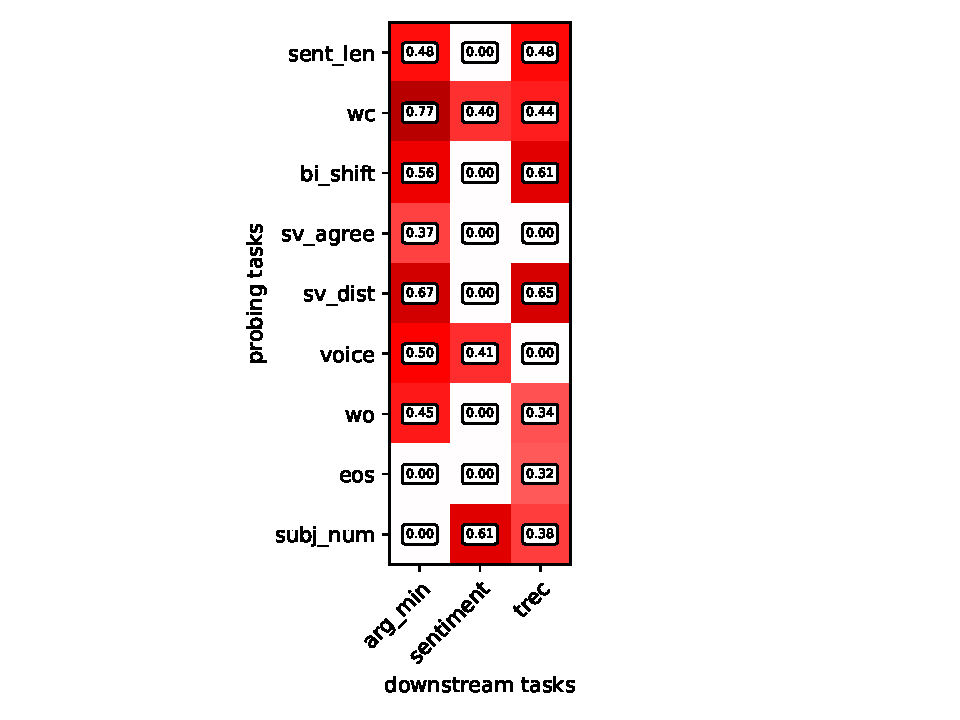
\includegraphics[scale=0.65]{images/spearman_corr_en_f1}
	\caption[Spearman correlations between probing and downstream task performances in English (F1 scores)]
		{Spearman correlations between probing and downstream task performances in English 
		\textbf{measured by F1 score}. \textcolor{red}{Reddish} values correspond to positive, \textcolor{blue}{blueish} values
		to negative correlations.}
	\label{fig:sp_corr_probing_downstream_en_f1}
\end{figure}

First of all, we notice that the correlations we obtained for the \caps{SentLen} task are rather high for \caps{TREC} and \caps{ArgMin}. This contradicts the finding reported by \citep{Conneau.2018a} who found that the \caps{SentLen} task is mainly negatively correlated with almost all downstream tasks (cf. figure \vref{fig:corr_conneau_perone}, left image). However, \citep{Eger.2019} have retrospectively correlated the results published by \citep{Perone.2018} and \textbf{found the exact opposite of what Conneau and colleagues report}. In this analysis, the \caps{SentLen} task shows the strongest connections to all downstream tasks on average (cf. figure \vref{fig:corr_conneau_perone}, right image). \citep{Eger.2019} conjecture that different sets of sentence embedding algorithms considered in the two papers are responsible for the divergence of the results. Conneau and colleagues use a set of related embeddings, whereas Perone et al. consider a more diverse set. \textbf{Different algorithms might focus on different linguistic aspects which influences the correlations.}

% Figure: Correlations by Conneau and Perone
\begin{figure}[h]
	\centering
	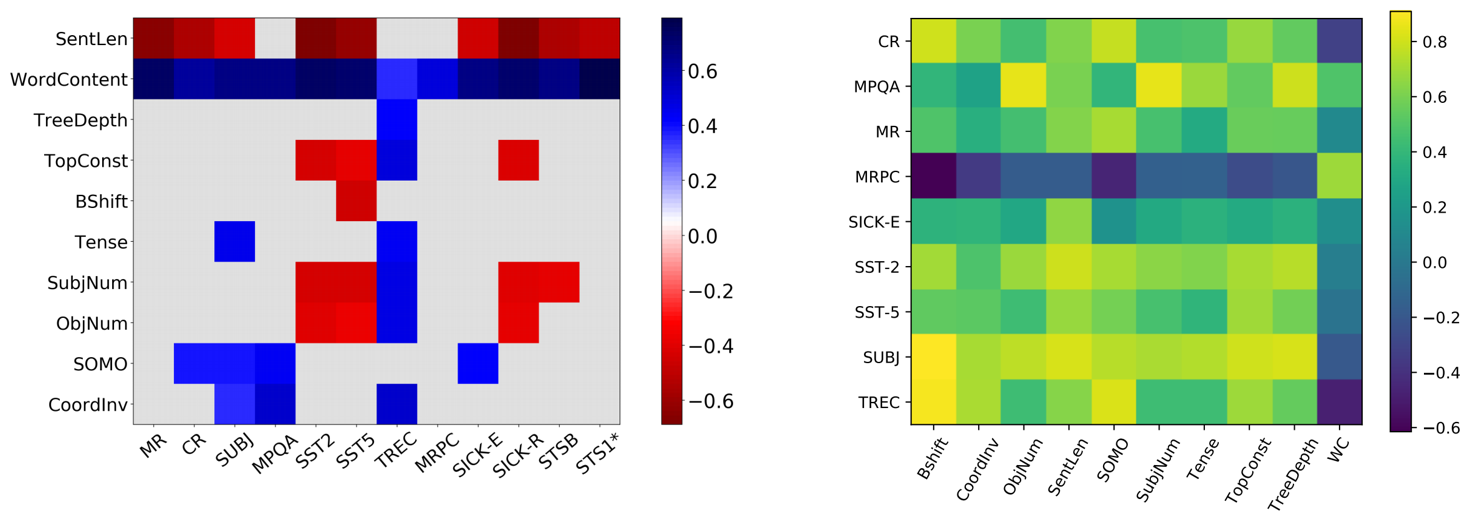
\includegraphics[scale=0.35]{images/corr_conneau_perone}
	\caption[Correlations between probing and downstream task performances from the literature]
		{Correlations between probing and downstream task performances from the literature.
		Left: Correlations reported by \citep{Conneau.2018a}. Please note that the color scheme is inverted.; 
		Right: Correlations of the results by \citep{Perone.2018}. The correlations were computed retrospectively by
		\citep{Eger.2019}.}
	\label{fig:corr_conneau_perone}
\end{figure}

% Table: Comparison of correlations with Krasnowska et al.
\begin{table}[h]
	\renewcommand{\arraystretch}{1.5}
	\centering
	\scalebox{1.0}{
	\begin{tabular}{ c c c c c c c c c c c c }
		\rotff{\textbf{Task}}							&
		\rotff{\textit{FastText\textsubscript{max}}} 		&
		\rotff{\textit{FastText\textsubscript{mean}}} 	&
		\rotff{\textit{BERT\textsubscript{max}}} 		&
		\rotff{\textit{BERT\textsubscript{mean}}} 		&
		\rotff{\textit{COMBO\textsubscript{max}}} 		&
		\rotff{\textit{COMBO\textsubscript{mean}}} 		&
		\rotff{\textit{sent2vec\textsubscript{ns}}} 		&
		\rotff{\textit{sent2vec\textsubscript{orig}}} 		&
		\rotff{\textit{LASER}} 						&
		\rotff{\textit{USE}} 							&
		\rotff{$\bm{r_s}$ \caps{Entail}}				\\
		\hline
		\textbf{\caps{SentLen}} 		& 52.55 & 72.27 & 72.66 & 82.13 & 85.03 & 87.38 & 71.56 & 64.76 & 85.98 & 60.00 
									& \textbf{-0.26} 	\\
		\hline
		\textbf{\caps{WC}} 			& 24.44 & 46.73 & 35.24 & 45.53 & 9.39 & 11.05 & 59.96 & 79.23 & 59.79 & 43.11
									& \textbf{0.72}	\\
		\hline
		\textbf{\caps{Voice}} 			& 84.13 & 89.47 & 89.77 & 92.40 & 98.48 & 98.41 & 88.73 & 89.04 & 92.85 & 86.61 
									& \textbf{-0.36}	\\
		\hline
		\textbf{\caps{SubjNum}}		& 73.87 & 81.43 & 88.43 & 90.75 & 93.19 & 93.37 & 82.27 & 80.88 & 94.21 & 81.65
									& \textbf{-0.02} 	\\
		\hline\hline
		\textbf{\caps{Entailment}}		& 76.72 & 76.86 & 77.71 & 77.11 & 72.82 & 72.58 & 78.59 & 78.26 & 83.26 & 81.77
									& -- \\
		\hline
	\end{tabular}}
	\caption[Results reported by Krasnowska et al. for several probing tasks as well as \caps{Entailment}]
		{Results reported by \citep{Krasnowska.2019} for several probing tasks as well as \caps{Entailment}.}
	\label{tab:comparison_correlation_krasnowska}
\end{table}

\textbf{Conneau and colleagues furthermore highlight the very strong positive correlations of the \caps{WC} task with all downstream applications.} This finding can be replicated in our experiment for the English language. This suggests that storing lexical information in the embeddings helps in downstream tasks. Consider for example the \caps{Senti} task, where the goal is to classify a sentence (or a snippet of text) into either positive or negative sentiment: If a sentence predominantly contains negatively (positively) connoted words, it is much more likely that this sentence also describes a negative (positive) sentiment. The \caps{ArgMin} task may serve as an additional example: The data set consists of sentences arguing either for or against a specific topic. If an embedding encodes information about argumentative words like e.\,g. \textit{`on the other hand'}, \textit{`likewise'}, \textit{`despite'}, \textit{`nevertheless'}, \textit{`as a consequence', etc.}, the classification of sentences into either supportive or confuting is accomplished much better. Finally, also the \caps{TREC} task profits from this knowledge: Storing information about the interrogative pronoun (question words like e.\,g. \textit{`what'}, \textit{`where'} and \textit{`how'}, etc.) directly gives hints as to what type of answer is expected. The results by \citep{Perone.2018}, on the other hand, indicate that knowledge about word containment is not as important for good performance in downstream applications \textbf{which sounds counter-intuitive}.

The correlations calculated by \citep{Conneau.2018a} furthermore indicate that detecting legal word orders is most of the time not indicative for good or bad performance in downstream applications. \textbf{Our results suggest a different conclusion:} The \caps{ArgMin} task as well as the \caps{TREC} task exhibit high correlations to the \caps{BiShift} probing task. This is compliant with the results by Perone et al. for which \citep{Eger.2019} compute a strong positive correlation of \caps{TREC} and \caps{BiShift}. We found that the closely related \caps{WO} task which also involves word order behaves analogously to \caps{BiShift}. \citep{Conneau.2018a} further point out that \textbf{the \caps{TREC} task has strong positive correlations with almost all probing tasks}. This finding can be reproduced in the context of our experiments. Only the tasks \caps{SVAgree} and \caps{Voice} are not connected to question type classification. Unfortunately, the \caps{SVAgree} task is not contained in the set of tasks introduced by Conneau et al., which is why a comparable figure is missing here.

\textbf{The \caps{Voice} task has positive correlations with the downstream tasks \caps{ArgMin} and \caps{Senti}}. If the accuracy metric is used (cf. figure \vref{fig:sp_corr_probing_downstream_en_acc}), the correlations become even stronger and \caps{Voice} is additionally correlated with \caps{TREC}. This suggests that voice information is helpful when it comes to performing well on downstream tasks. This finding is not intuitively obvious and the reasons for the importance of retaining voice information in sentence embeddings require further investigation. Unfortunately, this task is not included in the set of probing tasks shipped with \textit{SentEval}, but \citep{Krasnowska.2019} probed sentence embeddings using this task. The authors do not report probing task-downstream task correlations, but they report the accuracy values. Hence, it is possible to calculate the correlations retrospectively. The relevant results from their paper are summarized in table \vref{tab:comparison_correlation_krasnowska}. As can be seen from the table, the correlation between the probing task \caps{Voice} and the downstream task \caps{Entailment} is \textbf{negative}. \textbf{This means that \caps{Voice} is not always as predictive of downstream task performance as implied by the results we obtained.}

% Figure: Correlations between probing task / downstream task performance (en, accuracy)
\begin{figure}[h]
	\centering
	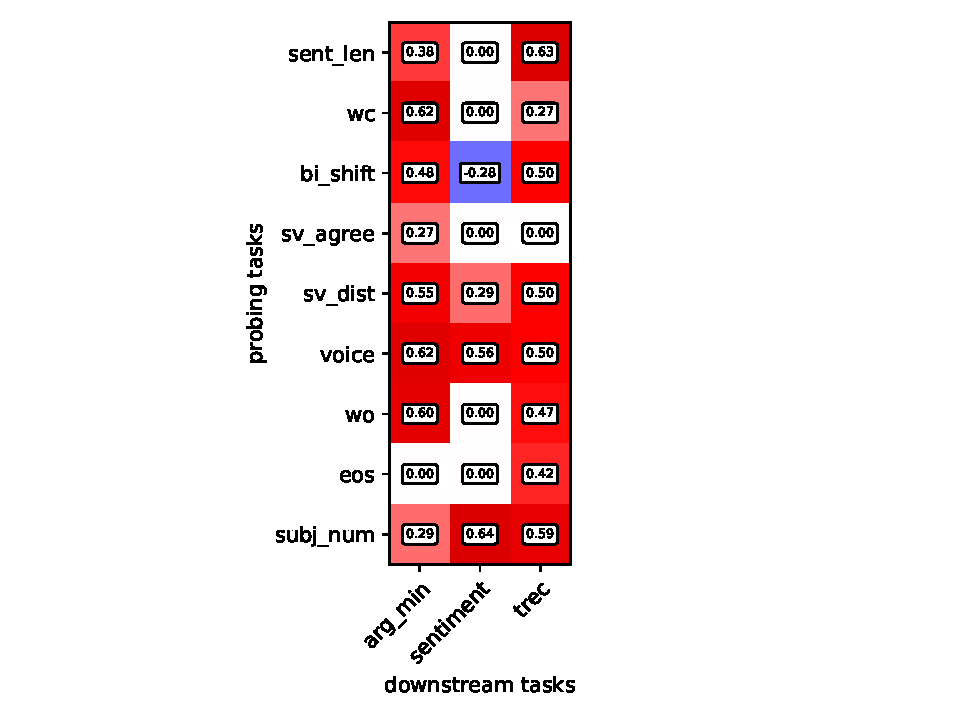
\includegraphics[scale=0.625]{images/spearman_corr_en_acc}
	\caption[Spearman correlations between probing and downstream task performances in English (accuracy)]
		{Spearman correlations between probing and downstream task performances in English 
		\textbf{measured by accuracy}. \textcolor{red}{Reddish} values correspond to positive, \textcolor{blue}{blueish} values
		to negative correlations.}
	\label{fig:sp_corr_probing_downstream_en_acc}
\end{figure}

\begin{tudbox}{Summary}
	\textbf{Many findings from the literature can be reproduced, yet differences can be observed due to different
	embeddings considered, different data sets or different probing and downstream tasks.}
\end{tudbox}

\highlight{Correlations in other languages.} The following paragraphs discuss the results for the remaining target languages, namely German, Russian, Turkish and Georgian. The figures \vref{fig:correlations_probing_downstream_de}, \vref{fig:correlations_probing_downstream_ru}, \vref{fig:correlations_probing_downstream_tr} and \vref{fig:correlations_probing_downstream_ka} show the respective results.

\textbf{The results for the other languages behave differently when compared to the English language.} In comparison to the English results, we notice first of all that a larger number of correlations is below an absolute value of 0.20, which is why they were set to 0.00. \textbf{What is more, many correlations have swapped into the negative range.} The strongest negative correlation can be observed for the Georgian \caps{WO} task, for which we computed a correlation with \caps{Senti} amounting to -0.73. Also the related \caps{BiShift} task shows a slight negative correlation with this downstream task in Georgian. The main reason for this may be the fact that it is possible to arrange words rather flexibly in the Georgian language (cf. section \vref{sec:georgian_language}), which renders the encoding of such information futile. Furthermore, an embedding has a finite number of dimensions. Encoding word order information might prevent the encoding of linguistic properties which are more relevant in the downstream tasks and might thus harm performance. While the \caps{TREC} task was reported to be correlated considerably positively with all probing tasks in the English language, \textbf{we could not reproduce this result in any of the other target languages}. The correlations for this task are either close to zero or negative. Furthermore, there are extremely strong positive correlations for the \caps{WC} task in German and less strong, but still noticeably positive correlations in Russian and Georgian. For the Turkish language we cannot confirm this finding: \textbf{There, the knowledge about word containment does not seem to be particularly decisive for downstream task performance}. This is surprising in light of the explanations given for the English language. In Turkish, the correlation between \caps{WC} and \caps{Senti} is even negative. This implies that either the explanations presented above are wrong, or they are at least not generalizable to all languages. Overall, the correlations in the Turkish language are less strong (except for the \caps{Senti} task with \caps{Voice} and \caps{SubjNum}). It is not entirely clear why this is the case for Turkish. 

% Figure: Correlations between probing task / downstream task performance (other languages: de, ru, tr, ka)
\begin{minipage}{0.49\textwidth}
	\begin{figure}[H]
		\centering
		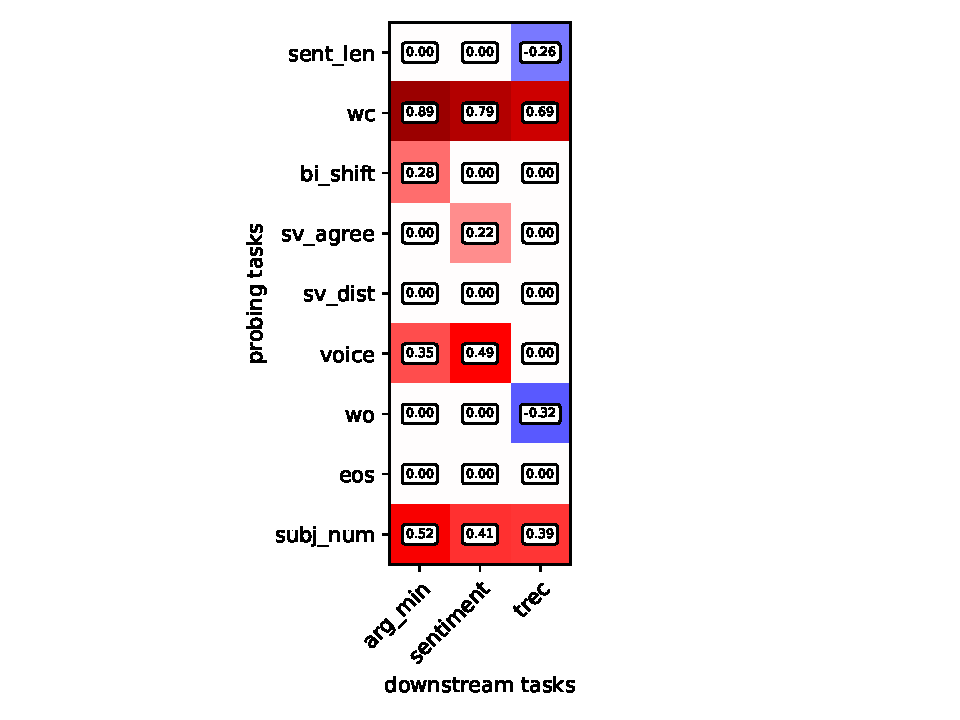
\includegraphics[scale=0.675]{images/spearman_corr_de_f1}
		\caption[Spearman correlations between probing and downstream task performances in German (F1 scores)]
			{Spearman correlations in German.}
		\label{fig:correlations_probing_downstream_de}
	\end{figure}
\end{minipage}
\hfill
\begin{minipage}{0.49\textwidth}
	\begin{figure}[H]
		\centering
		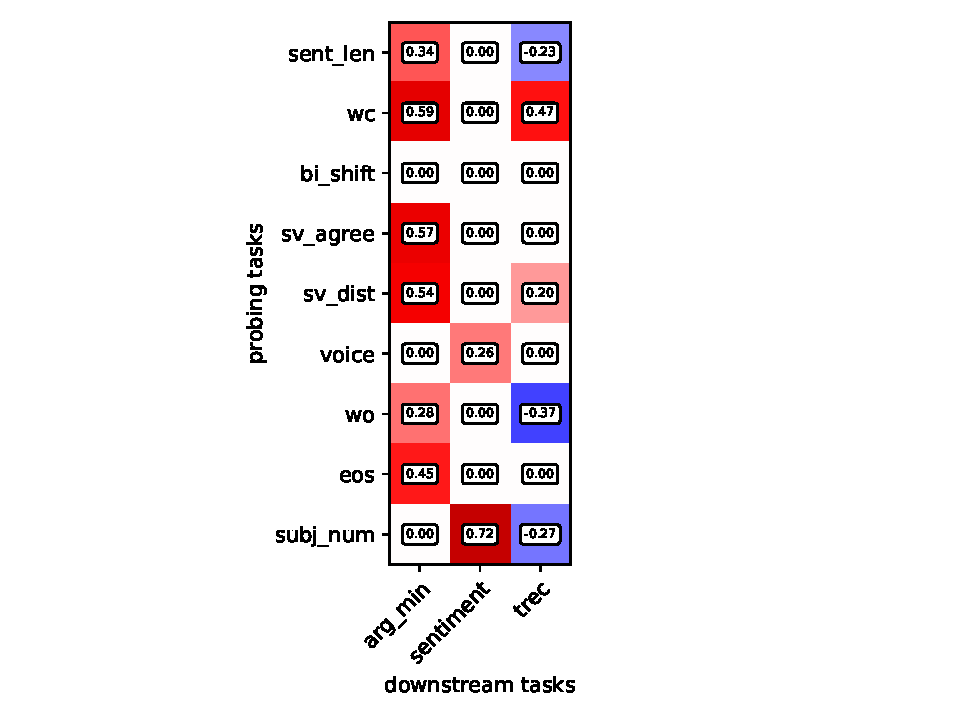
\includegraphics[scale=0.675]{images/spearman_corr_ru_f1}
		\caption[Spearman correlations between probing and downstream task performances in Russian (F1 scores)]
			{Spearman correlations in Russian.}
		\label{fig:correlations_probing_downstream_ru}
	\end{figure}
\end{minipage}

% Figure: Correlations between probing task / downstream task performance (other languages: de, ru, tr, ka)
\begin{minipage}{0.49\textwidth}
	\begin{figure}[H]
		\centering
		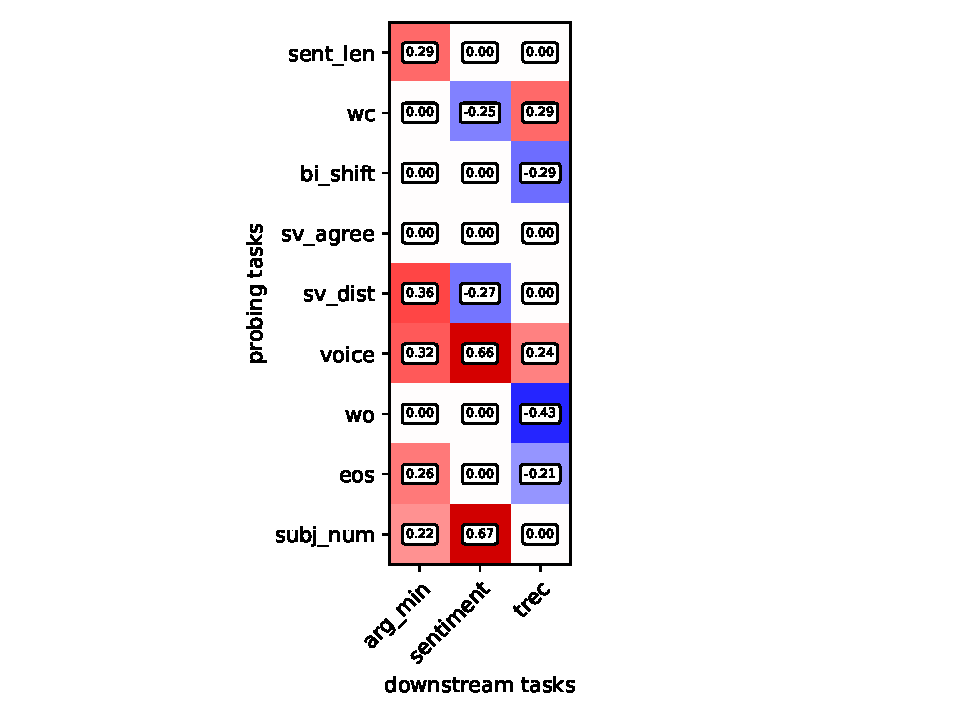
\includegraphics[scale=0.675]{images/spearman_corr_tr_f1}
		\caption[Spearman correlations between probing and downstream task performances in Turkish (F1 scores)]
			{Spearman correlations in Turkish.}
		\label{fig:correlations_probing_downstream_tr}
	\end{figure}
\end{minipage}
\hfill
\begin{minipage}{0.49\textwidth}
	\begin{figure}[H]
		\centering
		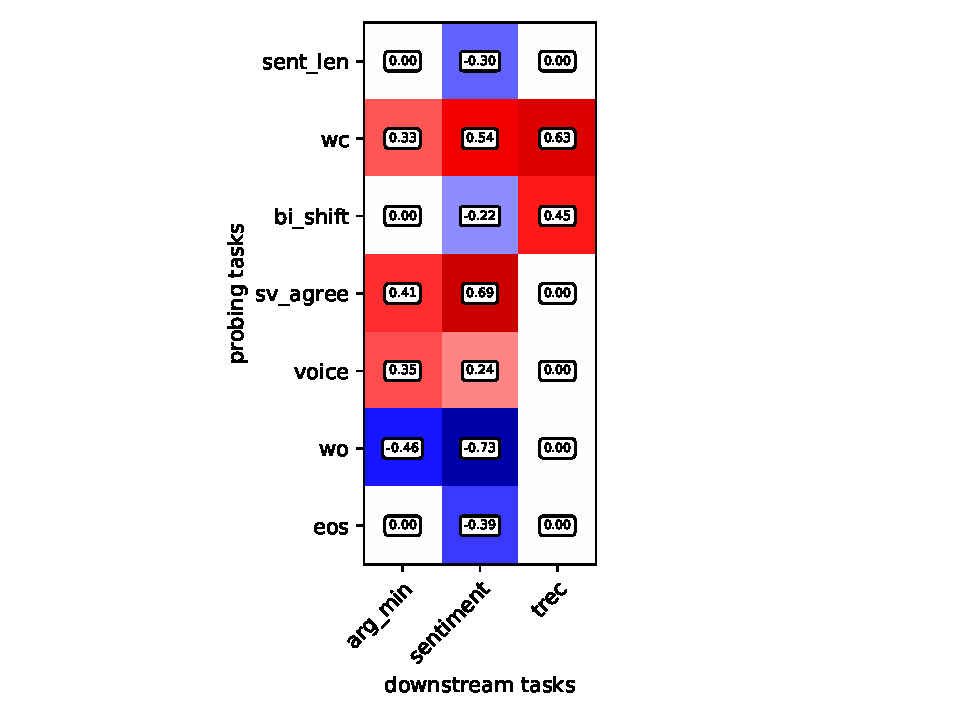
\includegraphics[scale=0.675]{images/spearman_corr_ka_f1}
		\caption[Spearman correlations between probing and downstream task performances in Georgian (F1 scores)]
			{Spearman correlations in Georgian.}
		\label{fig:correlations_probing_downstream_ka}
	\end{figure}
\end{minipage}

\vspace*{2mm}
\begin{tudbox}{Summary}
	\textbf{The results for the remaining languages are different compared to English. Many correlations have fallen below an absolute value of 0.20 or have swapped into the negative range entirely. The strongest negative correlation can be observed for the Georgian language. Also the correlations of the \caps{TREC} task with the set of probing tasks vanish. Turkish is the only language for which the knowledge about word containment is not predictive for downstream task performance.}
\end{tudbox}

\newpage
% -----------------------------------------------------------------------------------------------------------------------------------------------------
% Stability Analysis of the Embedding Ordering
\subsection{Stability Analysis of the Embedding Ordering}
\label{sec:stability_analysis}

One common problem in the evaluation of sentence embeddings on probing tasks is that different evaluation settings are used quite frequently. These differences are manifold: First of all, the size of the data sets are not standardized and vary as a consequence. Secondly, the research community did not agree on a single classifier type which is used to test the embeddings. Sometimes neural networks with a hidden layer are used, but also logistic regression is quite common. These two approaches differ in their representational power, thus influencing the final results. Furthermore, we detected settings where hyper-parameters like the number of hidden units or the dropout rate of an \gls{mlp} are tuned \citep{Conneau.2018a}, others use a fixed model architecture for the evaluation and do not mention hyper-parameter tuning explicitly \citep{Perone.2018}. I.\,e. it remains unclear whether or not they performed hyper-parameter optimization; and even if they did, they did not specify which hyper-parameters were tuned. Finally, the balance of the classes may have an influence on the performance of individual embeddings. On the one hand, \citep{Shi.2016} used an imbalanced \caps{Voice} data set for the evaluation (majority class amounts to 82.8\,\% for active voice), whereas, on the other hand, \citep{Conneau.2018a} created balanced data sets within the \textit{SentEval} framework. The data sets in this work are partially imbalanced (cf. tables \vref{tab:class_dist_probing_en_de}, \vref{tab:class_dist_probing_ru_tr} and \vref{tab:class_dist_probing_ka}), where especially the tasks \caps{SentLen} and \caps{WC} are concerned.

\textbf{These different setups motivated a detailed \textit{`stability analysis'} whose goal is \ding{182} to investigate the reasons for different results in this work and the literature, and \ding{183} to see which of the above mentioned factors have an influence on the ordering of the embeddings.} A review of the literature revealed that such a comprehensive study has not been conducted before. The following lines describe the experimental setup in greater depth: The analysis is performed for English and partially for Georgian using the example of the \caps{WC} task. The idea is to systematically change the factors of the evaluation setting one at a time (\textit{ceteris paribus}), such that the individual effects can be recorded. For reasons of time, it was not possible to perform this analysis exhaustively for all factor combinations. Instead, some combinations were picked and analyzed. The factors are as follows: \texttt{size} of the data set, \texttt{classifier}, \texttt{class balance} and \texttt{hyper-parameter tuning}.

\highlight{Factors \texttt{size} and \texttt{classifier}.} The first two factors which we investigate are \texttt{size} and \texttt{classifier}: We began by creating data sets of varying sizes for the \caps{WC} task. Since data sets which are too large require an excessive amount of computational resources, we decided to limit the size to a maximum of 60k instances. Four different data sets were created comprising 5k, 10k, 30k and 60k instances, respectively. The data sets were generated, such that data sets of smaller sizes are real subsets of larger data sets. \textbf{This entails that the 10k \caps{WC} task data set is not identical to the one used in earlier experiments. Hence, minor deviations in performance must be expected as a consequence.} The investigation of \texttt{classifier} effects requires that a set of diverse classification algorithms be chosen. To this end, we browsed the \textit{scikit-learn} library for adequate classifiers. The list below shows the classifiers which were used and also gives information with respect to the hyper-parameters used in the experiments:

\begin{tabbing}
	\hspace*{1cm}\=\hspace*{4cm}\=\hspace*{6cm}\=\kill
		\>	\textbf{Hyper-parameter}
		\>	\textbf{Argument}
		\>	\textbf{Explanation} 	\\[4mm]
	\ding{182} \textbf{Logistic regression (\texttt{LR})} 
		\>	\>	\> 	
\includegraphics[scale=0.02]{images/sklearn}									\\[3mm]
		\>	\texttt{C}			\>	3.75					\>	Regularization parameter			\\[3mm]
		\> 	\texttt{solver}		\>	lbfgs					\>	Optimization technique			\\[3mm]
		\>	\texttt{multi\_class}	\>	multinomial				\>	Multi-class setting					\\[4mm]
	\ding{183} \textbf{Random forest (\texttt{RF})}
		\>	\>	\> 	
\includegraphics[scale=0.02]{images/sklearn}									\\[3mm]
		\>	\texttt{n\_estimators}	\>	250						\>	Number of trees in the ensemble	\\[3mm]
		\>	\texttt{criterion} 		\>	gini						\>	Splitting heuristic					\\[3mm]
		\>	\texttt{max\_depth}	\>	70						\>	Maximum depth of single tree		\\[4mm]
	\ding{184} \textbf{Gaussian na\"{i}ve bayes (\texttt{NB})} 
		\>	\>	\> 	
\includegraphics[scale=0.02]{images/sklearn}									\\[3mm]
		\> 	no hyper-parameters 	\>							\>									\\[4mm]
	\ding{185} \textbf{Support vector machine (\texttt{SVM})}
		\>	\>	\> 	
\includegraphics[scale=0.02]{images/sklearn}									\\[3mm]
		\>	\texttt{kernel}		\>	linear					\>	Kernel type						\\[3mm]
		\>	\texttt{C}			\>	3.0						\>	Regularization parameter	\\[4mm]
	\ding{186} \textbf{Neural network without hidden layer (\texttt{NN})}
		\>	\>	\> 	
\includegraphics[scale=0.025]{images/keras}									\\[3mm]
		\>	\texttt{n\_epochs}	\>	100						\>	Number of training epochs			\\[3mm]
		\>	\texttt{loss} 			\>	categorical cross-entropy	\>	loss function							\\[3mm]
		\> 	\texttt{optimizer}		\> 	adam					\>	Optimization technique			\\[3mm]
		\> 	\texttt{act\_func} 	\>	sigmoid					\>	Activation function				\\[4mm]
	\ding{187} \textbf{Neural network with hidden layer (\texttt{NN\_H})}
		\>	\>	\> 	
\includegraphics[scale=0.025]{images/keras}									\\[3mm]
		\> 	\texttt{n\_hidden}	\>	50						\>	Number of neurons in hidden layer	\\[3mm]
		\> 	\texttt{drop\_out}	\>	0.00					\>	Dropout rate					\\[3mm]
		\> 	\textit{Other arguments equal to \texttt{NN}}\>		\>									\\
\end{tabbing}

These hyper-parameters were kept fixed for the factors \texttt{size} and \texttt{classifier} in the first half of this experiment. In order to obtain more stable results, we furthermore repeated the experiment, such that three individual results were available. The numbers listed in the following tables were produced by averaging the results over these three runs. Within each run we ensured that \textbf{all classifiers are evaluated on the same train-test splits across all embeddings} using an approach called \textbf{random subset evaluation}. Also, the random states of the classifiers were set, such that e.\,g. different weight initializations (for neural networks) or different attribute subset selections (for random forests) do not influence the results. \textbf{NB:} Results for the \gls{svm} classifier were produced only for 5k and 10k instances due to excessive computation time.

Table \vref{tab:corr_wc_en_clfs} shows the Spearman correlations obtained on the \caps{WC} task by using different \texttt{classifier}s, whereas table \vref{tab:corr_wc_en_sizes} focuses on correlations between varying data set \texttt{size}s. This evaluation serves two purposes: \ding{182} \textbf{Firstly, it is possible to determine a data set size for which no more considerable changes in the ranking of the embeddings take place.} \ding{183} \textbf{Secondly, the experiment allows for conclusions with respect to the rank stability of the embeddings across different classifiers.} We omitted detailed results here. In depth test results can be found in appendix \vref{sec:appendix_stability_analysis}).

% Figure: correlations word content English (10,000 instances, different classifiers)
\begin{table}[h]
	\centering
	\renewcommand{\arraystretch}{1.1}
	\scalebox{1.1}{
	\begin{tabular}{| l || c | c | c | c | c | c |}
		\hline
		\rowcolor{tud9c!50}
		\multicolumn{7}{| c |}{\textbf{10k instances (EN)}}		\\ \hline\hline
		\textbf{\texttt{LR}}		& 1.00 	& \gr 	& \gr 	& \gr	& \gr 	& \gr 	\\ \hline
		\textbf{\texttt{NN}}		& 0.91 	& 1.00 	& \gr 	& \gr	& \gr 	& \gr	\\ \hline
		\textbf{\texttt{NN\_H}}	& 0.83	& 0.94	& 1.00 	& \gr 	& \gr 	& \gr	\\ \hline
		\textbf{\texttt{RF}}		& 0.41	& 0.66	& 0.81	& 1.00 	& \gr 	& \gr	\\ \hline
		\textbf{\texttt{SVM}}		& 0.85	& 0.90	& 0.94	& 0.76	& 1.00 	& \gr	\\ \hline
		\textbf{\texttt{NB}}		& 0.84	& 0.83	& 0.76	& 0.34	& 0.78	& 1.00	\\ \hline\hline
		& \textbf{\texttt{LR}} & \textbf{\texttt{NN}} & \textbf{\texttt{NN\_H}} & \textbf{\texttt{RF}} & \textbf{\texttt{SVM}}
		& \textbf{\texttt{NB}} \\ \hline
	\end{tabular}}
	\caption[Spearman correlations for different classifiers (\caps{WC} task, EN, 10k instances)]
		{Spearman correlations computed for different classifiers (\caps{WC} task, EN, 10k instances).}
	\label{tab:corr_wc_en_clfs}
\end{table}

First of all consider the results reported in table \vref{tab:corr_wc_en_clfs} which shows the Spearman correlations of the embedding ordering when different classifiers are employed. The numbers in the table were produced on a fixed-sized data set comprising 10k instances. When looking at the numbers, we realize immediately that \textbf{the ordering of the embeddings is in general rather unstable across different classifiers} (correlations move in the range from 0.34 to 0.94). This holds especially true for the \texttt{RF} classifier for which the correlations deviate drastically from the remaining classifiers. We can reproduce this finding on the 5k, 30k and 60k data sets (cf. appendix \vref{sec:appendix_stability_analysis} for more information). Consistent lower correlations can also be observed for \texttt{NB}. Our experiments also show that neural architectures outperform the \texttt{RF} classifier and \texttt{NB}. For \textit{InferSent} embeddings on 60k instances we observed the following differences in performance: $\Delta$ \texttt{NN\_H} $\leftrightarrow$ \texttt{RF}/\texttt{NB} +0.21/+0.41 F1 score. (cf. table \vref{tab:results_en_wc_60000}). As expected, the correlation between the \texttt{LR} classifier and \texttt{NN} is noticeably positive, since both models are closely related. Also the positive correlation between the two neural architectures (\texttt{NN\_H} and \texttt{NN}) is considerable. \textbf{In summary, our results suggest that the choice of a specific classifier cannot be made blindly. Furthermore, classifiers like \texttt{NB} or \texttt{RF} should not be used, since they are consistently outperformed by neural architectures or logistic regression in our experiments.}

% Figure: correlations word content English (per classifier, different sizes)
\begin{table}[h]
	\begin{minipage}{0.32\textwidth}
		\begin{table}[H]
	\centering
	\scalebox{0.8}{
	\begin{tabular}{| l || c | c | c | c |}
		\hline
		\rowcolor{tud9c!50}
		\multicolumn{5}{| c |}{\textbf{\texttt{LR} classifier (EN)}}
		\\ \hline\hline
		\textbf{5k}		& 1.00 	& \gr 	& \gr 	& \gr 				\\ \hline
		\textbf{10k}		& 0.99 	& 1.00 	& \gr 	& \gr				\\ \hline
		\textbf{30k}		& 0.93	& 0.94	& 1.00 	& \gr 				\\ \hline
		\textbf{60k}		& 0.90	& 0.92	& 0.99	& 1.00				\\ \hline\hline
		& \textbf{5k} & \textbf{10k} & \textbf{30k} & \textbf{60k} 		\\ \hline
	\end{tabular}}
\end{table}
	\end{minipage}
	\hfill
	\begin{minipage}{0.32\textwidth}
		\begin{table}[H]
	\centering
	\scalebox{0.8}{
	\begin{tabular}{| l || c | c | c | c |}
		\hline
		\rowcolor{tud9c!50}
		\multicolumn{5}{| c |}{\textbf{\texttt{NN} classifier (EN)}}
		\\ \hline\hline
		\textbf{5k}		& 1.00 	& \gr 	& \gr 	& \gr 				\\ \hline
		\textbf{10k}		& 0.98 	& 1.00 	& \gr 	& \gr				\\ \hline
		\textbf{30k}		& 0.90	& 0.96	& 1.00 	& \gr 				\\ \hline
		\textbf{60k}		& 0.88	& 0.94	& 0.99	& 1.00				\\ \hline\hline
		& \textbf{5k} & \textbf{10k} & \textbf{30k} & \textbf{60k} 		\\ \hline
	\end{tabular}}
\end{table}
	\end{minipage}
	\hfill
	\begin{minipage}{0.32\textwidth}
		\begin{table}[H]
	\centering
	\scalebox{0.8}{
	\begin{tabular}{| l || c | c | c | c |}
		\hline
		\rowcolor{tud9c!50}
		\multicolumn{5}{| c |}{\textbf{\texttt{NN\_H} classifier (EN)}}
		\\ \hline\hline
		\textbf{5k}		& 1.00 	& \gr 	& \gr 	& \gr 				\\ \hline
		\textbf{10k}		& 0.95 	& 1.00 	& \gr 	& \gr				\\ \hline
		\textbf{30k}		& 0.87	& 0.94	& 1.00 	& \gr 				\\ \hline
		\textbf{60k}		& 0.84	& 0.92	& 0.99	& 1.00				\\ \hline\hline
		& \textbf{5k} & \textbf{10k} & \textbf{30k} & \textbf{60k} 		\\ \hline
	\end{tabular}}
\end{table}
	\end{minipage}

	\begin{minipage}{0.49\textwidth}
		\begin{table}[H]
	\centering
	\scalebox{0.8}{
	\begin{tabular}{| l || c | c | c | c |}
		\hline
		\rowcolor{tud9c!50}
		\multicolumn{5}{| c |}{\textbf{\texttt{RF} classifier (EN)}}
		\\ \hline\hline
		\textbf{5k}		& 1.00 	& \gr 	& \gr 	& \gr 				\\ \hline
		\textbf{10k}		& 0.99 	& 1.00 	& \gr 	& \gr				\\ \hline
		\textbf{30k}		& 0.97	& 0.97	& 1.00 	& \gr 				\\ \hline
		\textbf{60k}		& 0.97	& 0.97	& 1.00	& 1.00				\\ \hline\hline
		& \textbf{5k} & \textbf{10k} & \textbf{30k} & \textbf{60k} 		\\ \hline
	\end{tabular}}
\end{table}
	\end{minipage}
	\hfill
	\begin{minipage}{0.49\textwidth}
		\begin{table}[H]
	\centering
	\scalebox{0.8}{
	\begin{tabular}{| l || c | c | c | c |}
		\hline
		\rowcolor{tud9c!50}
		\multicolumn{5}{| c |}{\textbf{\texttt{NB} classifier (EN)}}
		\\ \hline\hline
		\textbf{5k}		& 1.00 	& \gr 	& \gr 	& \gr 				\\ \hline
		\textbf{10k}		& 1.00 	& 1.00 	& \gr 	& \gr				\\ \hline
		\textbf{30k}		& 0.94	& 0.94	& 1.00 	& \gr 				\\ \hline
		\textbf{60k}		& 0.92	& 0.92	& 0.99	& 1.00				\\ \hline\hline
		& \textbf{5k} & \textbf{10k} & \textbf{30k} & \textbf{60k} 		\\ \hline
	\end{tabular}}
\end{table}
	\end{minipage}
	\caption[Spearman correlations per classifier for different data set sizes (\caps{WC} task, EN)]
		{Spearman correlations per classifier computed for different data set sizes (\caps{WC} task, EN).}
	\label{tab:corr_wc_en_sizes}
\end{table}

Table \vref{tab:corr_wc_en_sizes} presents the rank stability with different data set sizes. We notice that for most of the classifiers, \textbf{the relative rankings between the embeddings change substantially between 5k training examples and a training set size of 60k instances}. Consider for example the numbers computed for the \texttt{NN\_H} classifier (top right), where the Spearman correlation between 5k and 60k instances amounting to 0.84 is rather low. At the same time, the correlation between 30k and 60k training examples is very close to 1.0 (also for the remaining classifiers). This means that the additional 30k training examples do not entail any noticeable changes in the ordering of the embeddings. \textbf{We therefore conclude that a data set size of 30k instances is sufficient to obtain a stable embedding ordering (at least on the \caps{WC} task in the English language).} For the \texttt{RF} classifier (bottom left), the correlations are already quite high between 5k and 60k training examples. \textbf{This means, that the ordering of the embeddings using this classifier is already relatively stable, even when training on small data sets.}

% Table: Embedding Ordering for 60,000 instances
\begin{table}[h]
	\centering
	\renewcommand{\arraystretch}{1.5}
	\scalebox{0.75}{
	\begin{tabularx}{1.3\textwidth}{| X ? Y | c ? Y | c ? Y | c ? Y | c ? Y | c |}
		\rowcolor{tud9c}
		\hline
																	&
		\multicolumn{2}{ c ?}{\textcolor{white}{\textbf{\texttt{LR}}}}	&
		\multicolumn{2}{ c ?}{\textcolor{white}{\textbf{\texttt{NN}}}	}	&
		\multicolumn{2}{ c ?}{\textcolor{white}{\textbf{\texttt{NN\_H}}}}&
		\multicolumn{2}{ c ?}{\textcolor{white}{\textbf{\texttt{RF}}}}	&
		\multicolumn{2}{ c |}{\textcolor{white}{\textbf{\texttt{NB}}}}	\\
		\multirow{-2}{*}{
			\cellcolor{tud9c}{\textcolor{white}{\textbf{60k instances}}}} 	&
		\cellcolor{tud9c!70}\textbf{F1} & \cellcolor{tud9c!70}\textbf{R} 	&
		\cellcolor{tud9c!70}\textbf{F1} & \cellcolor{tud9c!70}\textbf{R} 	&
		\cellcolor{tud9c!70}\textbf{F1} & \cellcolor{tud9c!70}\textbf{R} 	&
		\cellcolor{tud9c!70}\textbf{F1} & \cellcolor{tud9c!70}\textbf{R} 	&
		\cellcolor{tud9c!70}\textbf{F1} & \cellcolor{tud9c!70}\textbf{R} 	\\ \hline\hline

		Vanilla Average 	& 0.66 & 6 	& 0.78 & 8 	& 0.81 & 6 	& 0.31 & 9 	& 0.38 & 7 	\\ \hline
		GEM 			& 0.81 & 5 	& 0.81 & 5 	& 0.78 & 8 	& 0.36 & 8 	& 0.48 & 5 	\\ \hline
		SIF 				& 0.65 & 7 	& 0.79 & 7 	& 0.81 & 7 	& 0.38 & 7 	& 0.43 & 6 	\\ \hline
		p-Means 		& 0.45 & 10 	& 0.80 & 6 	& 0.82 & 4 	& 0.45 & 5 	& 0.23 & 9 	\\ \hline
		hier. pooling 		& 0.45 & 9 	& 0.51 & 12 	& 0.52 & 12 	& 0.24 & 11 	& 0.21 & 10	\\ \hline
		BOREP 			& 0.40 & 11 	& 0.66 & 10 	& 0.67 & 10 	& 0.59 & 3 	& 0.15 & 12	\\ \hline
		Random BiLSTM 	& 0.36 & 12 	& 0.68 & 9 	& 0.75 & 9 	& 0.30 & 10 	& 0.16 & 11	\\ \hline
		sent2vec 		& 0.83 & 4 	& 0.82 & 4 	& 0.81 & 5 	& 0.39 & 6 	& 0.64 & 1	\\ \hline
		Quick-Thought 	& 0.86 & 3 	& 0.92 & 2 	& 0.91 & 3 	& 0.57 & 4 	& 0.50 & 4	\\ \hline
		LASER 			& 0.88 & 2 	& 0.91 & 3 	& 0.92 & 2 	& 0.72 & 2 	& 0.55 & 3	\\ \hline
		BERT 			& 0.57 & 8 	& 0.59 & 11 	& 0.57 & 11 	& 0.22 & 12 	& 0.27 & 8	\\ \hline
		InferSent 		& 0.96 & 1 	& 0.97 & 1 	& 0.98 & 1 	& 0.77 & 1 	& 0.57 & 2	\\ \hline
	\end{tabularx}}
	\caption[Stability analysis results for 60k instances (\caps{WC} task, EN)]
		{Stability analysis results for 60k instances in (\caps{WC} task, EN).}
	\label{tab:results_en_wc_60000}
\end{table}

Table \vref{tab:results_en_wc_60000} shows detailed results of the embedding performances on the 60k data set: We see that the numbers for some of the embeddings are still not in the range reported by \citep{Perone.2018,Conneau.2018a}. Consider for instance the \textit{vanilla average} embedding for which Conneau and colleagues report 91.60\,\% accuracy on the \caps{WC} task. The result for the \texttt{NN\_H} classifier listed above (0.81) indicates that this still outperforms our score (the table shows F1 scores, the respective accuracy score on the data set is 86.31\,\%), although there are less classes in our setup. \textbf{Our results further suggest that the neural network without hidden layer (\texttt{NN}) performs worse than the \gls{mlp} (\texttt{NN\_H}).} \citep{Perone.2018,Conneau.2018a} removed the hidden layer for the evaluation on the \caps{WC} task because this gave better results in their experiments.\footnote{\citep{Conneau.2018a} refer to the \texttt{NN} classifier as logistic regression. This implementation must not be confused with \texttt{LR} which we adopted from the \textit{scikit-learn} library.} We were unable to observe this effect in our results. As table \vref{tab:results_en_wc_60000} reveals, the \texttt{NN} classifier is outperformed by the \texttt{NN\_H} classifier for 8 out of 12 embeddings. \textbf{The overall results suggest that the size of the data set as well as the classifier architecture are not the only effects to be made responsible for the deviations.} Before we examine the effects of the other factors (\texttt{class balance} and \texttt{hyper-parameter tuning}), we want to investigate whether the findings above can be reproduced for the Georgian language. In this context, the following results were obtained:

% Figure: correlations word content Georgian (10,000 instances, different classifiers)
\begin{table}[h]
	\centering
	\renewcommand{\arraystretch}{1.1}
	\scalebox{1.1}{
	\begin{tabular}{| l || c | c | c | c | c | c |}
		\hline
		\rowcolor{tud9c!50}
		\multicolumn{7}{| c |}{\textbf{10k instances (KA)}}		\\ \hline\hline
		\textbf{\texttt{LR}}		& 1.00 	& \gr 	& \gr 	& \gr	& \gr 	& \gr 	\\ \hline
		\textbf{\texttt{NN}}		& 0.88 	& 1.00 	& \gr 	& \gr	& \gr 	& \gr	\\ \hline
		\textbf{\texttt{NN\_H}}	& 0.89	& 0.98	& 1.00 	& \gr 	& \gr 	& \gr	\\ \hline
		\textbf{\texttt{RF}}		& 0.45	& 0.49	& 0.62	& 1.00 	& \gr 	& \gr	\\ \hline
		\textbf{\texttt{SVM}}		& 0.99	& 0.90	& 0.92	& 0.50	& 1.00 	& \gr	\\ \hline
		\textbf{\texttt{NB}}		& 0.61	& 0.76	& 0.71	& 0.13	& 0.60	& 1.00	\\ \hline\hline
		& \textbf{\texttt{LR}} & \textbf{\texttt{NN}} & \textbf{\texttt{NN\_H}} & \textbf{\texttt{RF}} & \textbf{\texttt{SVM}}
		& \textbf{\texttt{NB}} \\ \hline
	\end{tabular}}
	\caption[Spearman correlations for different classifiers (\caps{WC} task, KA, 10k instances)]
		{Spearman correlations computed for different classifiers (\caps{WC} task, KA, 10k instances).}
	\label{tab:corr_wc_ka_clfs}
\end{table}

% Figure: correlations word content Georgian (per classifier, different sizes)
\begin{table}[h]
	\begin{minipage}{0.32\textwidth}
		\begin{table}[H]
	\centering
	\scalebox{0.8}{
	\begin{tabular}{| l || c | c | c | c |}
		\hline
		\rowcolor{tud9c!50}
		\multicolumn{5}{| c |}{\textbf{\texttt{LR} classifier (KA)}}
		\\ \hline\hline
		\textbf{5k}		& 1.00 	& \gr 	& \gr 	& \gr 				\\ \hline
		\textbf{10k}		& 0.94 	& 1.00 	& \gr 	& \gr				\\ \hline
		\textbf{30k}		& 0.93	& 0.96	& 1.00 	& \gr 				\\ \hline
		\textbf{60k}		& 0.91	& 0.95	& 0.99	& 1.00				\\ \hline\hline
		& \textbf{5k} & \textbf{10k} & \textbf{30k} & \textbf{60k} 		\\ \hline
	\end{tabular}}
\end{table}
	\end{minipage}
	\hfill
	\begin{minipage}{0.32\textwidth}
		\begin{table}[H]
	\centering
	\scalebox{0.8}{
	\begin{tabular}{| l || c | c | c | c |}
		\hline
		\rowcolor{tud9c!50}
		\multicolumn{5}{| c |}{\textbf{\texttt{NN} classifier (KA)}}
		\\ \hline\hline
		\textbf{5k}		& 1.00 	& \gr 	& \gr 	& \gr 				\\ \hline
		\textbf{10k}		& 0.97 	& 1.00 	& \gr 	& \gr				\\ \hline
		\textbf{30k}		& 0.88	& 0.93	& 1.00 	& \gr 				\\ \hline
		\textbf{60k}		& 0.85	& 0.88	& 0.98	& 1.00				\\ \hline\hline
		& \textbf{5k} & \textbf{10k} & \textbf{30k} & \textbf{60k} 		\\ \hline
	\end{tabular}}
\end{table}
	\end{minipage}
	\hfill
	\begin{minipage}{0.32\textwidth}
		\begin{table}[H]
	\centering
	\scalebox{0.8}{
	\begin{tabular}{| l || c | c | c | c |}
		\hline
		\rowcolor{tud9c!50}
		\multicolumn{5}{| c |}{\textbf{\texttt{NN\_H} classifier (KA)}}
		\\ \hline\hline
		\textbf{5k}		& 1.00 	& \gr 	& \gr 	& \gr 				\\ \hline
		\textbf{10k}		& 0.99 	& 1.00 	& \gr 	& \gr				\\ \hline
		\textbf{30k}		& 0.87	& 0.91	& 1.00 	& \gr 				\\ \hline
		\textbf{60k}		& 0.72	& 0.77	& 0.94	& 1.00				\\ \hline\hline
		& \textbf{5k} & \textbf{10k} & \textbf{30k} & \textbf{60k} 		\\ \hline
	\end{tabular}}
\end{table}
	\end{minipage}

	\begin{minipage}{0.49\textwidth}
		\begin{table}[H]
	\centering
	\scalebox{0.8}{
	\begin{tabular}{| l || c | c | c | c |}
		\hline
		\rowcolor{tud9c!50}
		\multicolumn{5}{| c |}{\textbf{\texttt{RF} classifier (KA)}}
		\\ \hline\hline
		\textbf{5k}		& 1.00 	& \gr 	& \gr 	& \gr 				\\ \hline
		\textbf{10k}		& 0.99 	& 1.00 	& \gr 	& \gr				\\ \hline
		\textbf{30k}		& 0.97	& 0.97	& 1.00 	& \gr 				\\ \hline
		\textbf{60k}		& 0.97	& 0.97	& 1.00	& 1.00				\\ \hline\hline
		& \textbf{5k} & \textbf{10k} & \textbf{30k} & \textbf{60k} 		\\ \hline
	\end{tabular}}
\end{table}
	\end{minipage}
	\hfill
	\begin{minipage}{0.49\textwidth}
		\begin{table}[H]
	\centering
	\scalebox{0.8}{
	\begin{tabular}{| l || c | c | c | c |}
		\hline
		\rowcolor{tud9c!50}
		\multicolumn{5}{| c |}{\textbf{\texttt{NB} classifier (KA)}}
		\\ \hline\hline
		\textbf{5k}		& 1.00 	& \gr 	& \gr 	& \gr 				\\ \hline
		\textbf{10k}		& 0.94 	& 1.00 	& \gr 	& \gr				\\ \hline
		\textbf{30k}		& 0.95	& 0.98	& 1.00 	& \gr 				\\ \hline
		\textbf{60k}		& 0.97	& 0.99	& 0.99	& 1.00				\\ \hline\hline
		& \textbf{5k} & \textbf{10k} & \textbf{30k} & \textbf{60k} 		\\ \hline
	\end{tabular}}
\end{table}
	\end{minipage}
	\caption[Spearman correlations per classifier for different data set sizes (\caps{WC} task, KA)]
		{Spearman correlations per classifier computed for different data set sizes (\caps{WC} task, KA).}
	\label{tab:corr_wc_ka_sizes}
\end{table}

\textbf{Overall, the analysis of the embedding orderings using different classifiers yields a similar picture for Georgian compared to the English language} (cf. table \vref{tab:corr_wc_ka_clfs}): The \texttt{RF} classifier still exhibits the lowest correlation to all other classifiers. We observe the lowest correlation between \texttt{RF} and \texttt{NB} (0.13). Table \vref{tab:corr_wc_ka_sizes} furthermore confirms that \textbf{a data set size of approximately 30k instances is sufficient} in order to obtain a stable embedding ordering. Only the correlation between the sizes 30k and 60k for the \texttt{NN\_H} classifier amounts to a slightly smaller number (0.94) compared to English (cf. table \vref{tab:corr_wc_en_sizes}). An interesting observation is that the correlations for the \texttt{NB} classifier between 5k and 60k instances (0.97) is higher than between 5k and 10k (0.94) which means that the ordering changes when going from 5k to 10k, but approaches the original ranking again with more data.

\highlight{Factors \texttt{class balance} and \texttt{hyper-parameter tuning}.} The results produced for varying the factors data set \texttt{size} as well as \texttt{classifier} show that still certain differences persist between the evaluation results in this work and the literature. In the following paragraphs, we shift the focus towards the other two factors \texttt{class balance} and \texttt{hyper-parameter tuning} in the English language. As table \vref{tab:class_dist_probing_en_de} depicts, the data set for the \caps{WC} task we used previously is one among the most imbalanced ones. \textbf{For the following experiment, we therefore created a new 10k English data set with balanced classes.} To quantify the effect of \texttt{class balance} in combination with \texttt{size}, we further created balanced sets containing 30k and 60k instances, respectively. \textbf{Furthermore, we perform hyper-parameter optimization on these data sets.} Finally, we decided to apply the \texttt{NN} classifier as well, since we want to know whether the finding of \citep{Perone.2018,Conneau.2018a} (removing the hidden layer improves the performance on the \caps{WC} task) can be reproduced on balanced data. Figure \vref{fig:wc_detail_deltas} visualizes the absolute performance deltas in the various settings. We produced all results on the balanced 10k data set using the \texttt{NN\_H} classifier. Results for 30k and 60k training examples can be found in appendix \vref{sec:appendix_stability_analysis} (cf. table \vref{tab:wc_detail_deltas}).

% Figure: Delta performances
\begin{figure}[h]
\begin{minipage}{0.49\textwidth}
\begin{tikzpicture}
	\begin{axis}[
    		title=\textbf{\ding{182} class (im-)balance (10k)},
		ylabel=$\Delta$ F1 score,
		scale only axis,
		clip=false,
		separate axis lines,
		xtick={1,2,3,4,5,6,7,8,9,10,11,12},
        	x tick style={draw=none},
        	xticklabels={Average,p-Means,SIF,GEM,Hier. pooling,BOREP,rand. BiLSTM,InferSent,Quick-Th.,sent2vec,BERT,LASER},
		xticklabels={,,},
		width=7cm,height=3.25cm,
		tick label style={font=\scriptsize},
		xticklabel style={rotate=90},
		ymajorgrids,
    		grid style={line width=.1pt, draw=gray!10},
		ymin=0,
		every axis plot/.append style={
          		ybar,
          		bar width=8.0,
          		bar shift=0.5pt,
			fill
		},
		scaled y ticks=false,
		y tick label style={
        		/pgf/number format/.cd,
            		fixed,
            		fixed zerofill,
            		precision=2,
        		/tikz/.cd
    		}
	]

		\addplot[blue] coordinates {(1,0.21)};
     	 	\addplot[blue!80] coordinates {(2,0.20)};
      		\addplot[blue!60] coordinates {(3,0.24)};
      		\addplot[blue!40] coordinates {(4,0.17)};
		\addplot[blue!20] coordinates {(5,0.29)};
     	 	\addplot[gray] coordinates {(6,0.25)};
      		\addplot[lightgray] coordinates {(7,0.23)};
      		\addplot[red] coordinates {(8,0.07)};
     	 	\addplot[red!80] coordinates {(9,0.06)};
      		\addplot[red!60] coordinates {(10,0.22)};
      		\addplot[red!40] coordinates {(11,0.05)};
		\addplot[red!20] coordinates {(12,0.09)};
	\end{axis}
\end{tikzpicture}
\end{minipage}
\hfill
\begin{minipage}{0.49\textwidth}
\begin{tikzpicture}
	\begin{axis}[
    		title=\textbf{\ding{183} (no) hyper-parameter tuning (10k)},
		scale only axis,
		clip=false,
		separate axis lines,
		xtick={1,2,3,4,5,6,7,8,9,10,11,12},
        	x tick style={draw=none},
        	xticklabels={Average,p-Means,SIF,GEM,Hier. pooling,BOREP,rand. BiLSTM,InferSent,Quick-Th.,sent2vec,BERT,LASER},
		xticklabels={,,},
		width=7cm,height=3.25cm,
		tick label style={font=\scriptsize},
		xticklabel style={rotate=90},
		ymajorgrids,
    		grid style={line width=.1pt, draw=gray!10},
		ymin=0,
		every axis plot/.append style={
          		ybar,
          		bar width=8.0,
          		bar shift=0.5pt,
			fill
		},
		scaled y ticks=false,
		y tick label style={
        		/pgf/number format/.cd,
            		fixed,
            		fixed zerofill,
            		precision=2,
        		/tikz/.cd
    		}
	]

		\addplot[blue] coordinates {(1,0.05)};
     	 	\addplot[blue!80] coordinates {(2,0.02)};
      		\addplot[blue!60] coordinates {(3,0.05)};
      		\addplot[blue!40] coordinates {(4,0.03)};
		\addplot[blue!20] coordinates {(5,0.03)};
     	 	\addplot[gray] coordinates {(6,0.01)};
      		\addplot[lightgray] coordinates {(7,0.05)};
      		\addplot[red] coordinates {(8,0.01)};
     	 	\addplot[red!80] coordinates {(9,0.00)};
      		\addplot[red!60] coordinates {(10,0.01)};
      		\addplot[red!40] coordinates {(11,0.01)};
		\addplot[red!20] coordinates {(12,0.02)};
	\end{axis}
\end{tikzpicture}
\end{minipage}

\begin{minipage}{0.49\textwidth}
\begin{tikzpicture}
	\begin{axis}[
    		title=\textbf{\ding{184} \texttt{NN} $\leftrightarrow$ \texttt{NN\_H} (10k)},
		ylabel=$\Delta$ F1 score,
		scale only axis,
		clip=false,
		separate axis lines,
		xtick={1,2,3,4,5,6,7,8,9,10,11,12},
        	x tick style={draw=none},
        	xticklabels={Average,p-Means,SIF,GEM,Hier. pooling,BOREP,rand. BiLSTM,InferSent,Quick-Th.,sent2vec,BERT,LASER},
		width=7cm,height=3.25cm,
		tick label style={font=\scriptsize},
		xticklabel style={rotate=90},
		ymajorgrids,
    		grid style={line width=.1pt, draw=gray!10},
		every axis plot/.append style={
          		ybar,
          		bar width=8.0,
          		bar shift=0.5pt,
			fill
		},
		scaled y ticks=false,
		y tick label style={
        		/pgf/number format/.cd,
            		fixed,
            		fixed zerofill,
            		precision=2,
        		/tikz/.cd
    		}
	]

		\addplot[blue] coordinates {(1,-0.04)};
     	 	\addplot[blue!80] coordinates {(2,-0.03)};
      		\addplot[blue!60] coordinates {(3,-0.01)};
      		\addplot[blue!40] coordinates {(4,0.01)};
		\addplot[blue!20] coordinates {(5,-0.04)};
     	 	\addplot[gray] coordinates {(6,-0.01)};
      		\addplot[lightgray] coordinates {(7,-0.08)};
      		\addplot[red] coordinates {(8,-0.02)};
     	 	\addplot[red!80] coordinates {(9,-0.02)};
      		\addplot[red!60] coordinates {(10,0.00)};
      		\addplot[red!40] coordinates {(11,0.02)};
		\addplot[red!20] coordinates {(12,-0.08)};
	\end{axis}
\end{tikzpicture}
\end{minipage}
\hfill
\begin{minipage}{0.49\textwidth}
\begin{tikzpicture}
	\begin{axis}[
    		title=\textbf{\ding{185} size (10k $\leftrightarrow$ 30k)},
		scale only axis,
		clip=false,
		separate axis lines,
		xtick={1,2,3,4,5,6,7,8,9,10,11,12},
        	x tick style={draw=none},
        	xticklabels={Average,p-Means,SIF,GEM,Hier. pooling,BOREP,rand. BiLSTM,InferSent,Quick-Th.,sent2vec,BERT,LASER},
		width=7cm,height=3.25cm,
		tick label style={font=\scriptsize},
		xticklabel style={rotate=90},
		ymajorgrids,
    		grid style={line width=.1pt, draw=gray!10},
		ymin=0,
		every axis plot/.append style={
          		ybar,
          		bar width=8.0,
          		bar shift=0.5pt,
			fill
		},
		scaled y ticks=false,
		y tick label style={
        		/pgf/number format/.cd,
            		fixed,
            		fixed zerofill,
            		precision=2,
        		/tikz/.cd
    		}
	]

		\addplot[blue] coordinates {(1,0.09)};
     	 	\addplot[blue!80] coordinates {(2,0.08)};
      		\addplot[blue!60] coordinates {(3,0.07)};
      		\addplot[blue!40] coordinates {(4,0.01)};
		\addplot[blue!20] coordinates {(5,0.08)};
     	 	\addplot[gray] coordinates {(6,0.08)};
      		\addplot[lightgray] coordinates {(7,0.13)};
      		\addplot[red] coordinates {(8,0.02)};
     	 	\addplot[red!80] coordinates {(9,0.05)};
      		\addplot[red!60] coordinates {(10,0.01)};
      		\addplot[red!40] coordinates {(11,0.04)};
		\addplot[red!20] coordinates {(12,0.03)};
	\end{axis}
\end{tikzpicture}
\end{minipage}
\caption[Absolute F1 performance deltas in the \caps{WC} task (\texttt{NN\_H})]
	{Absolute F1 performance deltas in the \caps{WC} task (\texttt{NN\_H}):
	\ding{182} Effect of \texttt{class balance} (positive number indicates positive effect of balanced data),
	\ding{183} Effect of \texttt{hyper-parameter tuning} (on balanced data),
	\ding{184} Effect of \texttt{classifier} (on balanced data; negative values indicate worse performance of \texttt{NN}) and
	\ding{185} effect of \texttt{size} (on balanced data sets).}
\label{fig:wc_detail_deltas}
\end{figure}

\ding{182} \textbf{Effect of class (im-)balance.} Figure \vref{fig:wc_detail_deltas} (top left image) shows that \textbf{a balanced data set has positive effects on the performance of all embeddings}. We realized immediately that compositional models like the \textit{vanilla average} ($\Delta$ +0.21 F1), \textit{hierarchical pooling} ($\Delta$ +0.29 F1) or \textit{\gls{sif}} ($\Delta$ +0.24 F1) as well as random encoders profit the most from a balanced data set. Furthermore, the performance of \textit{sent2vec} is boosted considerably as well ($\Delta$ +0.22 F1). The scores of more sophisticated embeddings like \textit{InferSent} ($\Delta$ +0.07 F1), \textit{LASER} ($\Delta$ +0.09 F1) or \textit{Quick-Thought} ($\Delta$ +0.06 F1) are less influenced by a uniform class distribution and hardly change as a consequence. \textbf{The results suggest that the performance of averaging methods relies more on a balanced class distribution}. The performance improvement of \textit{sent2vec} is plausible in this context, since it is closely related to compositional models. \textbf{Conversely, this means that trained encoder architectures are more robust with respect to changes in the class distribution}.\footnote{At least in the \caps{WC} task in the English language.} This knowledge is essential, given the fact that in real-world applications, classes are rarely perfectly balanced. Such circumstances require the usage of robust embeddings which are also capable of handling data belonging to rare classes gracefully. As table \vref{tab:factor_effect_ranking} shows, also the embedding ranking is influenced by the \texttt{class balance} factor. We computed a Spearman correlation of 0.91. Detailed results can be found in table \vref{tab:wc_detail} in the appendix.

\ding{183} \textbf{Effect of hyper-parameter optimization.} Analogously to \citep{Conneau.2018a}, we implemented a hyper-parameter search over the parameters \texttt{\# hidden units} $\in \{ 50, 100, 200 \}$ and \texttt{dropout} $\in \{0, 0.1, 0.2 \}$. The 10k, 30k and 60k data sets were split into respective \texttt{train}, \texttt{dev} and \texttt{test} portions, where we used the \texttt{dev} set for the hyper-parameter optimization. Additionally, in order to prevent overfitting, an \textbf{early-stopping mechanism} on the \texttt{dev} set was introduced with the \texttt{patience} parameter set to a value of 5 (Conneau and colleagues also use early stopping). Figure \vref{fig:wc_detail_deltas} (top right image) reveals that \textbf{hyper-parameter tuning does not have a considerable impact on the performance of the embeddings}: The largest improvement can be observed for compositional and random models (especially the \textit{vanilla average}, \textit{SIF} and \textit{random BiLSTM} embeddings with $\Delta$ +0.05 F1 each). From table \vref{tab:factor_effect_ranking} we notice that the ranking of compositional models changes slightly, whereas the ranking of trained encoders is more robust. The Spearman correlation of the two rankings amounts to 0.95. Detailed results can be found in table \vref{tab:wc_detail_hp_opt} in the appendix.

% Table: Effect of class balance on embedding ordering
\begin{table}[h]
	\centering
	\renewcommand{\arraystretch}{1.1}
	\begin{tabular}{l c c c c c c c c c c c c}
									&
		\rotff{\textbf{Vanilla average}}		&
		\rotff{\textbf{p-Means}}			&
		\rotff{\textbf{SIF}}				&
		\rotff{\textbf{GEM}}				&
		\rotff{\textbf{hier. pooling}}		&
		\rotff{\textbf{BOREP}}			&
		\rotff{\textbf{Random BiLSTM}}		&
		\rotff{\textbf{InferSent}}			&
		\rotff{\textbf{Quick-Thought}}		&
		\rotff{\textbf{sent2vec}}			&
		\rotff{\textbf{BERT}}				&
		\rotff{\textbf{LASER}}				\\ \hline
		\multicolumn{13}{l}{\ding{182} \textbf{class (im-)balance}}											\\
		\textbf{Ranking} \textit{(imbalanced, 10k)}				& 8 & 6 & 7 & 5 & 12 & 9 & 11 & 1 & 3 & 4 & 9 & 2 	\\
		\textbf{Ranking} \textit{(balanced, 10k)}				& 8 & 7 & 6 & 5 & 11 & 9 & 10 & 2 & 4 & 1 & 12 & 3 	\\
		& \multicolumn{12}{c}{\textbf{Spearman correlation: 0.91}}											\\ \hline
		\multicolumn{13}{l}{\ding{183} \textbf{(no) hyper-parameter tuning}}									\\
		\textbf{Ranking} \textit{(balanced, no optimization, 10k)}	& 8 & 7 & 6 & 5 & 11 & 9 & 10 & 2 & 4 & 1 & 12 & 3 	\\
		\textbf{Ranking} \textit{(balanced, optimization, 10k)}		& 7 & 8 & 4 & 4 & 11 & 10 & 9 & 2 & 6 & 1 & 12 & 3 	\\
		& \multicolumn{12}{c}{\textbf{Spearman correlation: 0.95}}											\\ \hline
		\multicolumn{13}{l}{\ding{185} \textbf{size (10k $\leftrightarrow$ 30k)}}								\\
		\textbf{Ranking} \textit{(balanced, 10k)}				& 8 & 7 & 6 & 5 & 11 & 9 & 10 & 2 & 4 & 1 & 12 & 3 	\\
		\textbf{Ranking} \textit{(balanced, 30k)}				& 6 & 6 & 5 & 8 & 11 & 10 & 9 & 2 & 4 & 1 & 12 & 3 	\\
		& \multicolumn{12}{c}{\textbf{Spearman correlation: 0.94}}											\\ \hline
		\multicolumn{13}{l}{\ding{185} \textbf{size (30k $\leftrightarrow$ 60k)}}								\\
		\textbf{Ranking} \textit{(balanced, 30k)}				& 6 & 6 & 5 & 8 & 11 & 10 & 9 & 2 & 4 & 1 & 12 & 3 	\\
		\textbf{Ranking} \textit{(balanced, 60k)}				& 7 & 5 & 5 & 9 & 11 & 10 & 8 & 1 & 4 & 1 & 12 & 3 	\\
		& \multicolumn{12}{c}{\textbf{Spearman correlation: 0.98}}											\\ \hline
	\end{tabular}
	\caption[Effect of various factors on the embedding ranking]{Effect of various factors on the embedding ranking.}
	\label{tab:factor_effect_ranking}
\end{table}

\ding{184} \textbf{Effect of using the \texttt{NN} classifier on balanced data sets.} \citep{Conneau.2018a} as well as \citep{Perone.2018} stated that they removed the hidden layer for the \caps{WC} task, since this produced better results. \textbf{This effect could not be replicated before and also on balanced data sets we cannot observe this effect}: As figure \vref{fig:wc_detail_deltas} (bottom left image) shows, the \texttt{NN} classifier performs much worse for almost all embeddings (9 out of 12). However, this gap vanishes as the number of instances increases (cf. table \vref{tab:wc_detail_deltas} in the appendix): For 60k training examples, the \texttt{NN} model is mostly on par with the \texttt{NN\_H} classifier. Since Conneau and Perone used even more data, it is conceivable that the \texttt{NN} model might outperform the \texttt{NN\_H} classier on even larger data sets. Furthermore, their task was set up using 1k classes which can have an influence as well. Otherwise, this effect may be specific to the data set used by Conneau and Perone. Detailed results can be found in table \vref{tab:wc_detail} in the appendix.

\ding{185} \textbf{Effect of data set size on balanced data sets.} Our results suggest that \textbf{the data set size does have a positive effect on the performance} (cf. figure \vref{fig:wc_detail_deltas}; bottom right image), yet it is not as strong as the effect of balancing the class distribution. Again, compositional methods and random encoders improve a bit more compared to trained encoder architectures. While the ranking changes slightly between 10k and 30k instances (correlation of 0.94), it is rather stable between 30k and 60k instances for which we computed a correlation of 0.98 (cf. table \vref{tab:factor_effect_ranking}). This confirms the results obtained in the previous experiments, where a similar effect could be found. \textbf{This suggests that a probing task data set size of approximately 30k instances is sufficient to achieve a stable embedding ordering.} Detailed results can be found in table \vref{tab:wc_detail} in the appendix.

The last column of table \vref{tab:wc_detail_hp_opt} presents the final results obtained, if all additional effects are taken into account (using the \texttt{NN\_H} classifier on a large and balanced data set with hyper-parameter tuning enabled). These results come much closer to the ones reported in the literature (\textbf{NB:} different amount of classes). As the table reveals, most embeddings exhibit a performance greater than or equal to 0.90 F1 score (except for random encoders, \textit{BERT} and \textit{hierarchical pooling}) which implies that \textbf{the worse performances in the previous sections are caused by a combination of multiple effects}.

\textbf{Hyper-parameter optimization in other tasks.} The following table \vref{tab:effect_hp_other_tasks} lists the results obtained by conducting a hyper-parameter optimization on three other tasks, namely \caps{Senti}, \caps{Voice} and \caps{SubjNum}. This was done in order to exclude the possibility that the negligible effect of hyper-parameter tuning we found for \caps{WC} is specific to this task. \textbf{However, the table confirms the low impact of optimizing the hyper-parameters also in other tasks:} \textit{InferSent} profits the most on the \caps{Senti} task ($\Delta$ +0.05 F1 score); on \caps{Voice} it is \textit{LASER} and \textit{InferSent} ($\Delta$ +0.03 F1 score each), while \textit{Quick-Though} can improve the most on the \caps{SubjNum} task ($\Delta$ +0.04 F1 score).

% Effect of HP tuning in other tasks
\begin{table}[H]
	\centering
	\renewcommand{\arraystretch}{1.4}
	\scalebox{1.0}{
	\begin{tabular}{| c ? c | c | c ? c | c | c ? c | c | c |}
		\hline
		\rowcolor{tud9c}
		\multicolumn{10}{| c |}{\textcolor{white}{\textbf{Effect of hyper-parameter tuning on other tasks (original data sets)}}}
		\\ \hline
		\rowcolor{tud9c!70}
		\textbf{Task}								&
		\multicolumn{3}{ c ?}{\textbf{\caps{Senti}}} 		&
		\multicolumn{3}{ c ?}{\textbf{\caps{Voice}}} 		&
		\multicolumn{3}{ c |}{\textbf{\caps{SubjNum}}}
		\\ \hline
		\rowcolor{tud9c!50}
		\textbf{Tuning} &
		\textbf{yes} & \textbf{no} & $\bm{\Delta}$ &
		\textbf{yes} & \textbf{no} & $\bm{\Delta}$ &
		\textbf{yes} & \textbf{no} & $\bm{\Delta}$
		\\ \hline\hline
		Vanilla average		& 0.72 & 0.70 & \textbf{0.02} & 0.80 & 0.80 & \textbf{0.00} & 0.86 & 0.86 & \textbf{0.00} \\ \hline
		p-Means 			& 0.70 & 0.70 & \textbf{0.00} & 0.83 & 0.81 & \textbf{0.02} & 0.88 & 0.85 & \textbf{0.03} \\ \hline
		BOREP 			& 0.65 & 0.65 & \textbf{0.00} & 0.80 & 0.78 & \textbf{0.02} & 0.87 & 0.84 & \textbf{0.03} \\ \hline
		Random BiLSTM 	& 0.69 & 0.69 & \textbf{0.00} & 0.84 & 0.83 & \textbf{0.01} & 0.88 & 0.88 & \textbf{0.00} \\ \hline
		InferSent 			& 0.75 & 0.70 & \textbf{0.05} & 0.90 & 0.87 & \textbf{0.03} & 0.91 & 0.88 & \textbf{0.03} \\ \hline
		Quick-Thought 		& 0.67 & 0.64 & \textbf{0.03} & 0.83 & 0.81 & \textbf{0.02} & 0.80 & 0.76 & \textbf{0.04} \\ \hline
		sent2vec 			& 0.66 & 0.66 & \textbf{0.00} & 0.78 & 0.78 & \textbf{0.00} & 0.77 & 0.76 & \textbf{0.01} \\ \hline
		BERT 			& 0.65 & 0.64 & \textbf{0.01} & 0.78 & 0.76 & \textbf{0.02} & 0.88 & 0.86 & \textbf{0.02} \\ \hline
		LASER 			& 0.74 & 0.73 & \textbf{0.01} & 0.93 & 0.90 & \textbf{0.03} & 0.92 & 0.90 & \textbf{0.02} \\ \hline
	\end{tabular}}
	\caption[Effect of hyper-parameter tuning in other tasks]{Effect of hyper-parameter tuning in other tasks (measured by F1 score).}
	\label{tab:effect_hp_other_tasks}
\end{table}

\begin{tudbox}{Summary}
\textbf{Large (at least 30k examples) and balanced data sets have a substantial positive effect on the performance of the embeddings. Hyper-parameter tuning, on the other hand, was found to be of minor importance (observed on several tasks). Overall, we found that compositional models profit the most. The results furthermore suggest to use neural architectures for the evaluation, since such models consistently outperform other classifiers in terms of absolute scores.}
\end{tudbox}

% -----------------------------------------------------------------------------------------------------------------------------------------------------
% Discussion, limitations and recommendations for future work
\subsection{Discussion, Limitations and Recommendations for future Work}
\label{sec:discussion}

\highlight{Research question \ding{182}.} The results of the analyses presented in this chapter demonstrate that \textbf{trained encoders are superior to compositional models or random encoders in English}. Nevertheless, as \citep{Wieting.2019} already found out, random encoders provide a very strong baseline and the gap to trained architectures is often smaller than desirable. \textbf{This gap vanishes even more in low-resource languages:} A lack of sufficient amounts of training data on which the encoder architectures can be trained, ultimately entails worse performance. As a consequence, compositional embeddings and random encoders are sometimes able to outperform trained models in such settings. Despite worse absolute scores, the top-three analysis reveals that trained embeddings can still have advantages if resources are scarce. Also, in order to check whether low-quality translations have a considerable  influence on the performance in low-resource languages, it might be worthwhile to check their trustworthiness. The translated sentences could be translated back into English to see whether or not the results differ substantially from the original sentences.

\textbf{The results obtained in this work further confirm that, independently of the language, still no universal sentence embedding exists:} The performance of the embeddings strongly depends on the task at hand which means that there is no embedding which consistently shows strong performance \citep{Perone.2018}. \textit{LASER}, however, scores highly across many tasks and languages and can therefore be considered close to a universal sentence embedding. It has the advantage that it was trained on high-quality and multilingual corpora which did not have to be translated. Also \textit{InferSent} shows convincing performances for the English language. In the other languages, however, its scores should be treated with caution, since the models were not trained on the full \textit{AllNLI} data set which impairs the performance. Therefore, we should continue the translation process and retrain the models, once the full data set is available in all target languages.

\textbf{Surprisingly, we found that high-dimensional embeddings do not necessarily have advantages in the evaluation on probing tasks.} Negative correlations between embedding dimensionality and performance in some of the probing tasks suggest that low-dimensional embeddings can achieve better scores than high-dimensional ones. \textbf{Also, we notice that there is much more variance in the probing task performances in comparison to the downstream task results.} We hold the artificial setup of probing tasks accountable for this circumstance. This result can also be found in the paper by \citep{Perone.2018}.

The correlations computed between probing and downstream task results (cf. section \vref{sec:correlation_probing_downstream_tasks}) suggest for the English language that the \textbf{knowledge about word containment is a strong predictor of downstream task performance}. Also \caps{Voice} is correlated positively with most of the downstream applications considered. In this context we found some inconsistencies with results in the literature. However, \citep{Eger.2019} report that the correlations depend on the set of embeddings considered in the analysis. Additionally, we detected that the language has an influence on the ultimate results: \textbf{The correlations for the other target languages behave differently compared to English:} The \caps{TREC} task for which we computed high positive correlations in English does not have substantial connections to the probing tasks in the remaining languages. Also, we found many negative values. The strongest negative correlation could be found for the Georgian \caps{WO} task. We believe that the flexible word order in the Georgian language is responsible for this.

\highlight{Research question \ding{183}.} Different setups in the literature and our work caused discrepancies which we attempted to analyze more in depth: \textbf{One of the main findings in this context was that it is crucial to evaluate the embeddings on balanced probing task data sets} (cf. section \vref{sec:stability_analysis}). Especially compositional models were found to profit from such a setting and as a consequence improve up to almost 0.30 F1 score (cf. \textit{hierarchical pooling}). Imbalanced data sets therefore cause a distortion between compositional and trained sentence embedding models (the rankings change considerably). Naturally, the choice of using balanced or imbalanced data sets depends on the research questions to be addressed. In reality, data sets are rarely balanced, i.\,e. if the embeddings are supposed to be tested in a more realistic scenario, the data sets would have to be imbalanced. However, probing tasks were especially designed to test sentence representations in a laboratory environment which assumes perfect conditions. In addition, the size of the probing task data set matters: \textbf{We detected that at least 30k instances should be used in order to get a stable embedding ordering.} \fbox{\textbf{The stability analysis suggests that our results should be treated with caution:}} The results reported in this work were produced on 10k data sets which are partially imbalanced. The reason for this is that it turned out to be very difficult to create large data sets for the low-resource languages. In the interest of comparability, we decided to limit the size of the data sets to 10k also for the English language. In future work, more effort should be put into the creation of larger and balanced probing task data sets.

While the factors \texttt{class balance} and \texttt{size} have substantial influence on the performance on probing tasks, we found that \textbf{\texttt{hyper-parameter tuning} only accounts for minor improvements} which could be replicated in several tasks. Finally, the ordering of the embeddings is partially very unstable across different classifiers but neural architectures consistently outperform other models like random forests in terms of absolute scores. \textbf{Finally, we give the following recommendations for a good probing task setup in future work:}

\begin{tudbox}{Recommendations for future work}
% recommendations
\begin{enumerate}[label=\color{tud9c}\textbf{\theenumi.}]
	\setlength\itemsep{2.4em}
	\item Probing task data sets should comprise at least \textbf{30k instances}.
	\item The data sets should be \textbf{balanced}.
	\item The probing task classifier should be a \textbf{neural network} (preferably an \gls{mlp}).
	\item Optionally, hyper-parameter tuning can be used despite of only slight positive effects \\
		(it does not hurt the performance).
\end{enumerate}
\end{tudbox}

Some of the recommendations, especially the creation of large and balanced data sets, are challenging to implement for low-resource languages like Georgian. Fortunately, additional \textit{\gls{ud}} tree banks for the Georgian language will be available soon. This data can be used to create even better data sets for the probing tasks. Despite the detailed analysis, some of the discrepancies still remain: E.\,g. the performance of the \textit{power means} embedding on the \caps{WC} task is still lower compared to \citep{Perone.2018}, despite less classes in our setup. Explanations for this circumstance are speculative and require further analysis (even larger data sets?, embedding dimension?). Also, we still notice differences on the \caps{TREC} task. \textbf{In order to enable a smoother comparison with the literature, we recommend that future work in this domain makes use of the \textit{SentEval} framework.} Furthermore, we have to make sure that the embeddings to be tested are produced using the same hyper-parameter settings as in the literature (same embedding dimensionalities, window sizes, ...).

The evaluation setups in the literature mostly respect the recommendations given above and the setup we implemented should have been more oriented towards the evaluation protocol used in the literature. Nonetheless, the stability analysis clearly demonstrates that the the ultimate evaluation results depend on the setting to a large extent. \textbf{We posit that the evaluation should be agnostic with respect to external factors like class balance or the number of training examples. Since the encoder architectures are frozen, the representations for single sentences do not change as a consequence of larger or balanced probing task data sets. Therefore, it is not entirely clear to us, what the probing task results indicate. We hope that future work in this area will provide clarification.}

% Chapter Summary
% -----------------------------------------------------------------------------------------------------------------------------------------------------
\subsection{Summary}
\label{sec:results_eval_summary}

This chapter provided details about the evaluation results on probing and downstream tasks. Section \vref{sec:results_probing_tasks} first of all presented the probing task results while the subsequent section \vref{sec:results_downstream_tasks} focused on downstream task performances. As soon as the embeddings were evaluated intrinsically (probing tasks) as well as extrinsically (downstream tasks), we could correlate the results in order to get clarity about which linguistic properties are decisive for downstream tasks performance (cf. section \vref{sec:correlation_probing_downstream_tasks}). It was shown that the correlations vary between the languages.

Since the evaluation is not performed consistently in the literature and also to investigate discrepancies in the context of this work, an additional stability analysis was performed (cf. section \vref{sec:stability_analysis}). In this experiment, various factors (data set \texttt{size}, \texttt{class balance}, \texttt{classifier} architectures and \texttt{hyper-parameter optimization}) were changed systematically and the influence on the performances was recorded. Based on the outcomes of this analysis, we gave recommendations w.\,r.\,t. a better evaluation setup for future work (cf. section \vref{sec:discussion})
